%% This is the ctufit-thesis example file. It is used to produce theses
%% for submission to Czech Technical University, Faculty of Information Technology.
%%
%% This is version 1.6.0, built 18. 9. 2025.
%% 
%% Get the newest version from
%% https://gitlab.fit.cvut.cz/theses-templates/FITthesis-LaTeX
%%
%%
%% Copyright 2024, Tomas Novacek
%% Copyright 2021, Eliska Sestakova and Ondrej Guth
%%
%% This work may be distributed and/or modified under the
%% conditions of the LaTeX Project Public License, either version 1.3
%% of this license or (at your option) any later version.
%% The latest version of this license is in
%%  https://www.latex-project.org/lppl.txt
%% and version 1.3 or later is part of all distributions of LaTeX
%% version 2005/12/01 or later.
%%
%% This work has the LPPL maintenance status `maintained'.
%%
%% The current maintainer of this work is Tomas Novacek (novacto3@fit.cvut.cz).
%% Alternatively, submit bug reports to the tracker at
%% https://gitlab.fit.cvut.cz/theses-templates/FITthesis-LaTeX/issues
%%
%%

% arara: xelatex
% arara: biber
% arara: xelatex
% arara: xelatex

%%%%%%%%%%%%%%%%%%%%%%%%%%%%%%%%%%%%%%%%%
% CLASS OPTIONS
% language: czech/english/slovak
% thesis type: bachelor/master/dissertation/doctoral-report
% electronic (oneside) or printed (twoside), twoside is default
% paragraph - if passed, this optional argument sets paragraphs as the deepest level of headers, styles it, numbers it and adds it to Table of Content. Use with care! Normally, it is considered unwise to use it, since it is too deep.
% colour: bw for black&white OR no option for default colour scheme
%%%%%%%%%%%%%%%%%%%%%%%%%%%%%%%%%%%%%%%%%
\documentclass[english,master,oneside]{ctufit-thesis}

%%%%%%%%%%%%%%%%%%%%%%%%%%%%%%%%%%
% FILL IN THIS INFORMATION
%%%%%%%%%%%%%%%%%%%%%%%%%%%%%%%%%%
\ctufittitle{Design and Implementation of a Scalable, On-Premise Infrastructure for Large-Scale Data Gathering, Processing, and Storage in Machine Learning Applications}
\ctufitauthorfull{Bc. Jan Troják}
\ctufitauthorsurnames{Troják}
\ctufitauthorgivennames{Jan}
\ctufitsupervisor{Ing. Tomáš Vondra\, Ph.D.}
\ctufitdepartment{Department of Computer Systems}
\ctufitprogram{Informatika}
\ctufitspecialisation{Computer Systems and Networks}
\ctufityear{2026}
\ctufitdeclarationplace{Prague}
\ctufitdeclarationdate{\today}
\ctufitabstractCZE{Tato práce popisuje návrh soukromého výpočetního prostředí pro shromažďování a analýzu velkých sbírek digitálních obrazů. Systém řeší běžný problém s efektivitou, kdy správa milionů jednotlivých malých položek způsobuje zpomalení systémů kvůli administrativní zátěži. Díky volbě specializované metody ukládání, která uchovává informace o adresářích v rychlé paměti a seskupuje položky do větších balíčků, systém zajišťuje téměř okamžitý přístup k jakémukoliv souboru. Toto nastavení bylo vytvořeno na specializovaném fyzickém hardwaru, aby bylo možné plně kontrolovat soukromí dat a náklady a vyhnout se nutnosti veřejného internetového úložiště.

Druhá část práce představuje automatizovaný zpracovatelský proces, který umožňuje transformaci dat, například výpočet obrazových reprezentací. Tento proces je navržen tak, aby byl vysoce dostupný a škálovatelný na základě pracovní zátěže. Díky použití automatizovaných škálovacích mechanismů systém aktivně přizpůsobuje své zdroje v závislosti na objemu příchozích úkolů, čímž udržuje vysokou propustnost během špiček a zároveň optimalizuje efektivitu při nízké zátěži.}
\ctufitabstractENG{This thesis describes the design of a private computing environment for gathering and analyzing large collections of digital images. The system solves a common efficiency problem where managing millions of individual small items causes systems to slow down due to administrative overhead. By choosing a specialized storage method that keeps the directory information in fast memory and groups items into larger packages, the system ensures nearly instant access to any single item. This setup was built on dedicated physical hardware to provide full control over data privacy and costs, avoiding the need for public internet-based storage.

The second part of the thesis presents an automated processing pipeline that enables data transformation, such as computing image representations. This pipeline is designed to be highly available and scalable based on the workload. Through the use of automated scaling mechanisms, the system actively adjusts its resources in response to the volume of incoming tasks, maintaining high throughput during peak periods while optimizing efficiency when the load is low.}
\ctufitkeywordsCZE{Infrastruktura strojového učení, Zpracování obrazu, Distribuované ukládání dat, Problém malých souborů, Datové potrubí, On-premise řešení, Automatické škálování}
\ctufitkeywordsENG{Machine learning infrastructure, Image processing, Distributed data storage, Small file problem, Data pipelines, On-premise solutions, Performance autoscaling}
%%%%%%%%%%%%%%%%%%%%%%%%%%%%%%%%%%
% END FILL IN
%%%%%%%%%%%%%%%%%%%%%%%%%%%%%%%%%%

%%%%%%%%%%%%%%%%%%%%%%%%%%%%%%%%%%
% CUSTOMIZATION of this template
% Skip this part or alter it if you know what you are doing.
%%%%%%%%%%%%%%%%%%%%%%%%%%%%%%%%%%

\RequirePackage{iftex}[2020/03/06]
\iftutex % XeLaTeX and LuaLaTeX
    \RequirePackage{ellipsis}[2020/05/22] %ellipsis workaround for XeLaTeX
\else
    \errmessage{Only compilation with XeLaTeX or LuaLaTeX is allowed}
    \stop
\fi

% hyperlinks
\hypersetup{
    pdfpagelayout=TwoPageRight,
    colorlinks=true,
    allcolors=decoration,
    pdfborder={0 0 0}
}

% uncomment the following to hide all hyperlinks
%\hypersetup{hidelinks}

% uncomment the following to change the colour of all hyperlinks to CTU blue
\hypersetup{allbordercolors=decoration}

\RequirePackage{pdfpages}[2020/01/28]

%%%%%%%%%%%%%%%%%%%%%%%%%%%%%%%%%%
% CUSTOMIZATION of this template END
%%%%%%%%%%%%%%%%%%%%%%%%%%%%%%%%%%


%%%%%%%%%%%%%%%%%%%%%%
% PACKAGES SETTINGS
% You may choose to modify this part.
%%%%%%%%%%%%%%%%%%%%%%
\usepackage{dirtree}
\usepackage{lipsum,tikz}
\usepackage{newtxtt} % Better monospaced font with TU encoding support
\usepackage{fontspec}        % Základ pro XeLaTeX/LuaLaTeX
\usepackage{polyglossia}     % Náhrada za Babel pro moderní překladače
\setmainlanguage{english}    % Hlavní jazyk
\setotherlanguage{czech}     % Vedlejší jazyk
\usepackage[style=iso-numeric]{biblatex}
\setcounter{biburlucpenalty}{8000}
\addbibresource{./dt.bib}
\usepackage{xurl}
\usepackage{multicol}
\usepackage{enumitem}
\usepackage{graphicx}
% \usepackage{listings} % typesetting of sources
%\usepackage{minted}
% \usepackage{microtype}
\usepackage{csquotes}
\usepackage{tgcursor}
%%%%%%%%%%%%%%%%%%%%%%
% PACKAGES SETTINGS END


\newcommand{\term}[1]{\mbox{\texttt{#1}}}
\setlength{\bibitemsep}{1em}
\begin{document}
\frontmatter\frontmatterinit % do not remove these two commands

\thispagestyle{empty}\maketitle\thispagestyle{empty}\cleardoublepage

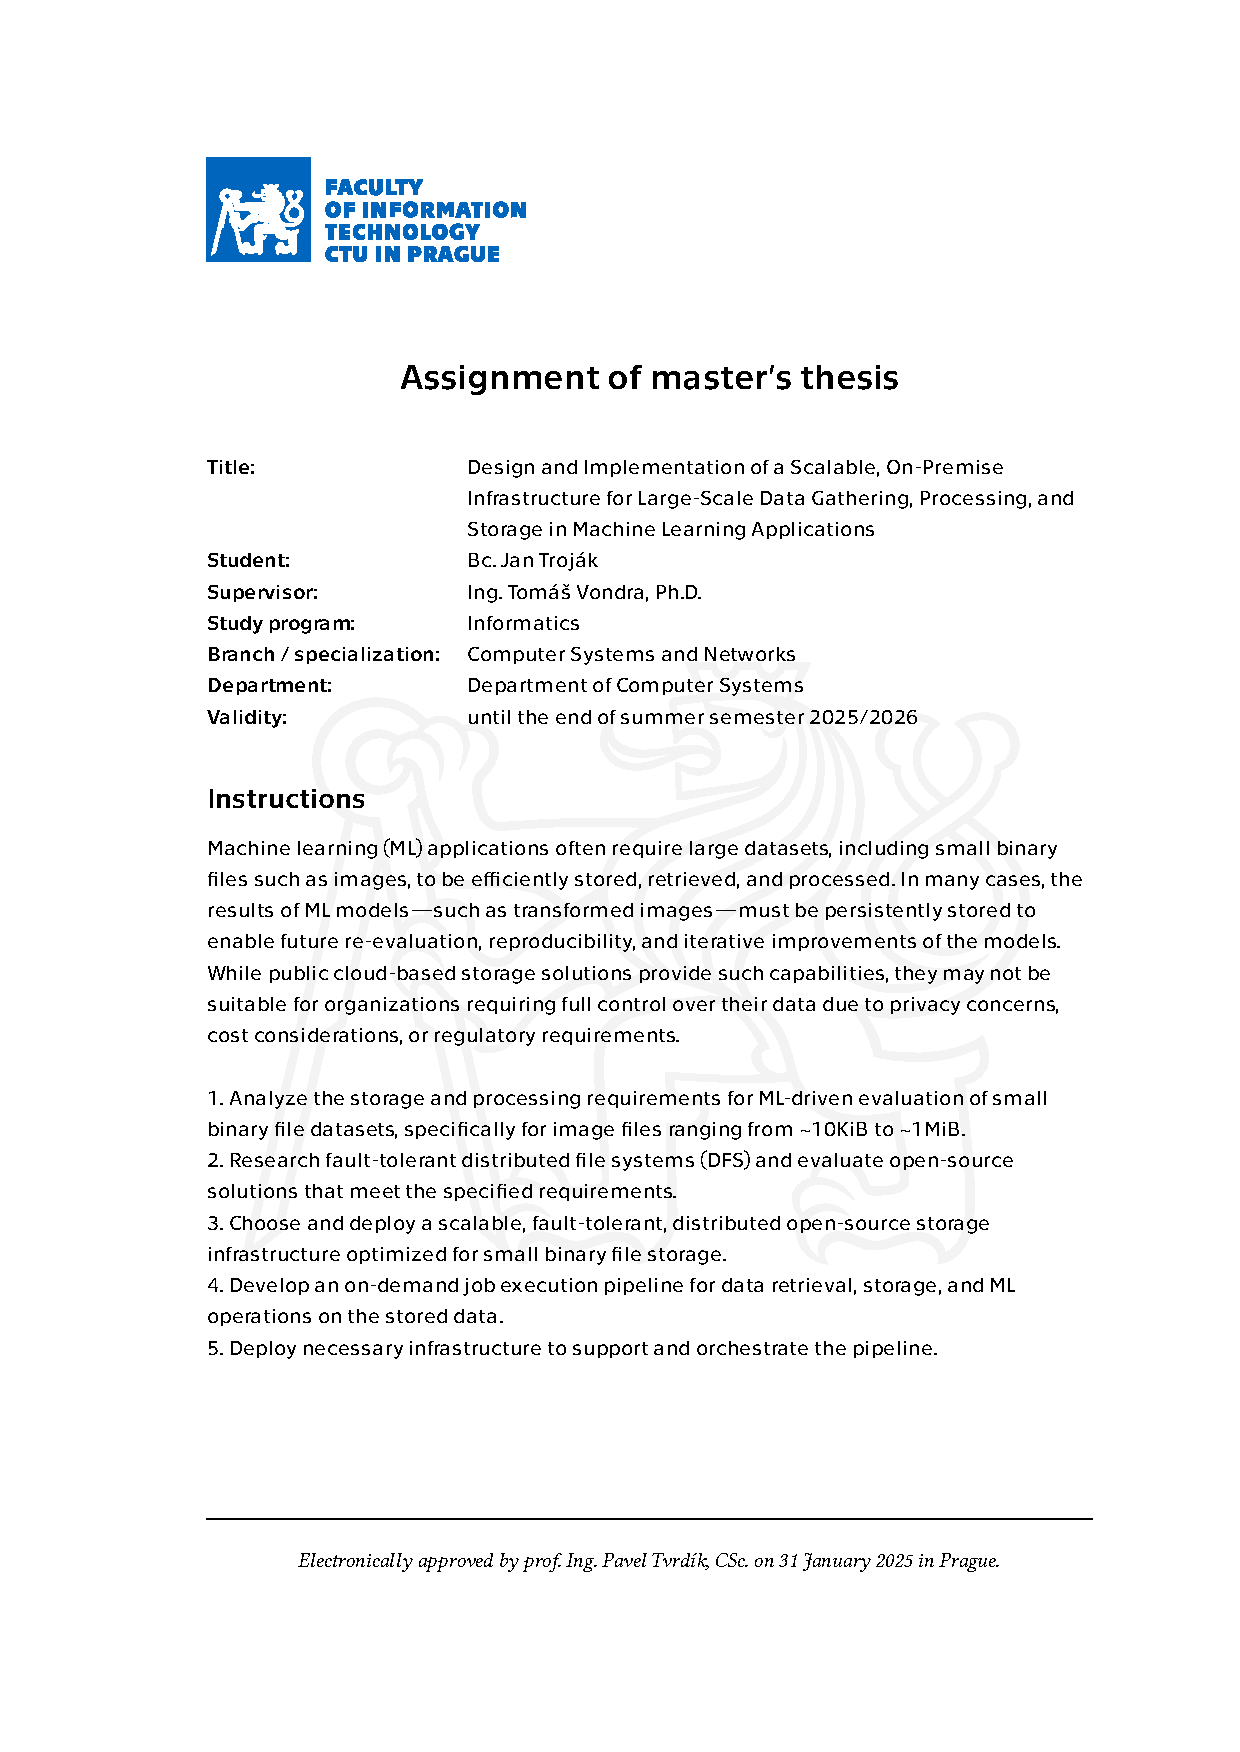
\includepdf[pages={1-}]{trojaj12-assignment.pdf} % replace this file with your thesis assignment generated from ProjectsFIT

\imprintpage % do not remove this command
\stopTOCentries

%%%%%%%%%%%%%%%%%%%
% ACKNOWLEDGMENT
% FILL IN / MODIFY
% This is a place to thank people for helping you. It is common to thank your supervisor.
%%%%%%%%%%%%%%%%%%%

%%%%%%%%%%%%%%%%%%%
% ACKNOWLEDGMENT END
%%%%%%%%%%%%%%%%%%%


%%%%%%%%%%%%%%%%%%%
% DECLARATION
% FILL IN / MODIFY
%%%%%%%%%%%%%%%%%%%
% INSTRUCTIONS
% ENG: choose one of approved texts of the declaration. DO NOT CREATE YOUR OWN. Find the approved texts at https://courses.fit.cvut.cz/SFE/download/index.html#_documents (document Declaration for FT in English)
% CZE/SLO: Vyberte jedno z fakultou schvalenych prohlaseni. NEVKLADEJTE VLASTNI TEXT. Schvalena prohlaseni najdete zde: https://courses.fit.cvut.cz/SZZ/dokumenty/index.html#_dokumenty (prohlášení do ZP)
\begin{declarationpage}
I hereby declare that the presented thesis is my own work and that I have cited all sources of
information in accordance with the Guideline for adhering to ethical principles when elaborating an
academic final thesis.

I acknowledge that my thesis is subject to the rights and obligations stipulated by the Act No.
121/2000 Coll., the Copyright Act, as amended. In accordance with Section 2373(2) of Act No.
89/2012 Coll., the Civil Code, as amended, I hereby grant a non-exclusive authorization (licence) to
utilize this thesis, including all computer programs that are part of it or attached to it and all
documentation thereof (hereinafter collectively referred to as the "Work"), to any and all persons
who wish to use the Work. Such persons are entitled to use the Work in any manner that does not
diminish the value of the Work and for any purpose (including use for profit). This authorisation is
unlimited in time, territory and quantity

I declare that I have used AI tools during the preparation and writing of my thesis. I have verified
the generated content. I confirm that I am aware that I am fully responsible for the content of the
thesis.
\end{declarationpage}

%%%%%%%%%%%%%%%%%%%
% DECLARATION END
%%%%%%%%%%%%%%%%%%%

% Use one of the two following commands. The first prints abstracts+keywords on two pages, the second puts them on one page (if possible). \printonepageabstract can also accept optional argument that specifies a vertical space before both abstracts (the default is 18 mm).
\printtwopageabstract
%\printonepageabstract 

%%%%%%%%%%%%%%%%%%%
% SUMMARY
% FILL IN / MODIFY
% OR REMOVE ENTIRELY (upon agreement with your supervisor)
% (appropriate to remove in most theses)
%%%%%%%%%%%%%%%%%%%
% \begin{summarypage}
% \section*{Summary section}
% 
% \lipsum[1][1-8]
% 
% \section*{Summary section}
% 
% \lipsum[2][1-6]
% 
% \section*{Summary section}
% 
% \lipsum[3]
% 
% \section*{Summary section}
% 
% \lipsum[2]
% 
% \section*{Summary section}
% 
% \lipsum[1][1-8] Lorem lorem lorem.
% \end{summarypage}
%%%%%%%%%%%%%%%%%%%
% SUMMARY END
%%%%%%%%%%%%%%%%%%%

\tableofcontents % do not remove this command
%%%%%%%%%%%%%%%%%%%%%%
% list of other contents: figures, tables, code listings, algorithms, etc.
% add/remove commands accordingly
%%%%%%%%%%%%%%%%%%%%%%
\listoffigures % list of figures
\begingroup
\let\clearpage\relax
\listoftables % list of tables. Remove if you do not have any.
% \thectufitlistingscommand{} % list of code listings. Remove if you do not have any.
\thectufitlistofalgorithmscommand{} % list of algorithm pseudocodes defined using the algorithm package.
\endgroup
%%%%%%%%%%%%%%%%%%%%%%
% list of other contents END
%%%%%%%%%%%%%%%%%%%%%%

%%%%%%%%%%%%%%%%%%%
% ABBREVIATIONS
% FILL IN / MODIFY
% OR REMOVE ENTIRELY
% List the abbreviations in lexicography order.
%%%%%%%%%%%%%%%%%%%
\chapter{\thectufitabbreviationlabel}
{
    \definecolor{myAcronymColor}{RGB}{0, 0, 0}
    \fontsize{10pt}{12pt}\selectfont
    \begin{description}[
        font=\normalfont\bfseries\color{myAcronymColor}, 
        nosep,                       % No vertical space between items
        align=right,                 % Align shortcuts to the left
        labelwidth=4.5em,            % Fixed width for the shortcut column
        leftmargin=12.0em,           % labelwidth + some padding for the description
    ]
        \item[AI] Artificial Intelligence
        \item[API] Application Programming Interface
        \item[CNCF] Cloud Native Computing Foundation
        \item[CRD] Custom Resource Definition
        \item[CSI] Container Storage Interface
        \item[DAG] Directed Acyclic Graph
        \item[DB] Database
        \item[DNS] Domain Name System
        \item[DRBD] Distributed Replicated Storage System
        \item[FS] File System
        \item[HA] High Availability
        \item[IaC] Infrastructure as Code
        \item[ID] Identifier
        \item[IO] Input/Output
        \item[IOPS] Input/Output Operations Per Second
        \item[LVM] Logical Volume Manager
        \item[ML] Machine Learning
        \item[NFS] Network File System
        \item[NHR] National High-Performance Computing
        \item[OSD] Object Storage Device
        \item[POSIX] Portable Operating System Interface
        \item[QoS] Quality of Service
        \item[RADOS] Reliable Autonomic Distributed Object Store
        \item[REST] Representational State Transfer
        \item[SDK] Software Development Kit
        \item[SDN] Software-Defined Networking
        \item[SDStorage] Software-Defined Storage
        \item[SDSys] Software-Defined System
        \item[SSD] Solid State Drive
        \item[UI] User Interface
        \item[ZFS] Zettabyte File System
        
    \end{description}
}
%%%%%%%%%%%%%%%%%%%
% ABBREVIATIONS END
%%%%%%%%%%%%%%%%%%%
\resumeTOCentries
\mainmatter\mainmatterinit % do not remove these two commands
%%%%%%%%%%%%%%%%%%%
% THE THESIS
% MODIFY ANYTHING BELOW THIS LINE
%%%%%%%%%%%%%%%%%%%

% Do not forget to include the Introduction
%---------------------------------------------------------------
% uncomment the following line to create an unnumbered chapter
%\chapter*{Introduction}\addcontentsline{toc}{chapter}{Introduction}\markboth{Introduction}{Introduction}
%---------------------------------------------------------------
\setcounter{page}{1}

\input{text/chapters/01_part}
\chapter{Introduction} \label{sec:introduction}
\section{Problem Declaration} \label{ch:problem_declaration}
Modern AI systems that work with user images must do two things reliably: keep the raw images safe, organized, quickly retrievable; run repeatable processing on those images, e.g., annotation and embedding (see Section \ref{sec:image_embeddings}\footnote{Terms like embeddings are explained later in the image processing chapter of the thesis (\ref{sec:image_processing}).}). In practice, this typically requires building a data storage that persists a large number of small binary files. In addition to storage, data processing pipelines are constructed to execute jobs on data and process them as needed.

The first operational aspect of image processing systems is the design of the storage system. The problem of storing a large number of small binary files (images) does not fit the requirements for which traditional storage solutions were designed. Storing a large number of small files can lead to significant overhead in metadata management, which can cause poor performance on traditional systems.\cite{beaver_finding_2010}

For an image store, it is crucial to minimize metadata management overhead, enable parallel read (and possibly write) operations to serve data efficiently, and focus on systems that prioritize reading over writing and deletion. At the same time, customer and regulatory constraints often rule out the public cloud, requiring full control and on-premises deployment. Among other needs, the solution must typically be fault-tolerant and highly available.

On the computation side, there are mixed requirements from online and offline processing. For offline processing, it is necessary to ensure fault tolerance and limit the number of errors during computation. Offline processing often computes large amounts of data in one bulk operation, in case of backfills or recomputation when a model changes. Bulk operations require careful scheduling of resources to deliver the largest throughput possible, but keep the price of such computation reasonably low. On the other hand, online computations focus on low latency and high availability. This leads to an auto-scaling computation solution within the hard limits of an on-premises cluster. The processing pipeline must be idempotent and resumable in the event of failure, enabling failure recovery. Finally, computed artifacts need to be persistently stored and indexed with metadata and a backlink to its original source.

\section{Motivation} \label{sec:motivation}
The motivation for this thesis is driven by a significant and growing industry need to build reliable image-processing pipelines that can operate at a massive scale. Modern machine learning applications, particularly in domains such as e-commerce, recommendation systems, and search, increasingly depend on the ability to efficiently process and analyze large image datasets. Providing a solution that can ingest, store and process millions of items is a challenge to serving the needs of large, data-intensive systems.

This thesis is directly motivated by a real-world business requirement from Recombee, a company specializing in AI-powered recommendation systems. Such systems should enable the company to develop improved recommendations and AI-powered search systems. Such a system is a key component in supporting more sophisticated content-based recommendations and search functionalities that rely on a deep understanding of visual data, rather than just provided metadata.

The challenge of efficiently managing and storing a massive volume of small binary files, often referred to as \textit{the Small File Problem}, is not unique to the primary use case of this thesis. It is a common challenge in many other data-intensive industries. For example, large-scale e-commerce platforms must manage billions of product images, and social media networks must store vast amounts of user-generated photos. Therefore, the results and research on the storage component of the thesis can be valuable for other use cases when developing such on-premises storage infrastructure, particularly for small binary files.

The second part of the thesis (developing a data processing pipeline) can also serve as inspiration for other implementations of similar use cases, where a data processing pipeline is required. Such systems could be similar to AI-processing, model training, etc.

\section{Purpose} \label{sec:purpose}
The purpose of this thesis is to design and implement an on-premises infrastructure that makes large-scale image processing possible. In practice, the work aims to provide a fault-tolerant storage solution for handling large numbers of small images ($\approx$10 KiB to 1 MiB) and to build an automated, on-demand job-execution pipeline that scales ML operations, such as embedding computations. This involves first analyzing the specific storage and processing requirements for such datasets, then researching and deploying a suitable scalable, fault-tolerant, distributed open-source storage infrastructure, and finally developing and deploying the necessary pipeline.
\chapter{Image processing} \label{sec:image_processing}
\section{Image Embeddings} \label{sec:image_embeddings}
The embedding process involves transforming (encoding) a data source into a high-dimensional vector. This vector is called a \textit{vector embedding}, sometimes shortened to embedding, which refers to the final product of the embedding process. More abstractly, it is described as a mathematical function from one data space to another (representation) space $f: X \to Z$, where $X$ is the space of data, $Z$ is the space of representation, and $f$ is a function performing such a translation, see Figure \ref{fig:embedding}. In the concrete model, which describes the use case for this thesis, $X$ denotes the space of images (small binary files), $Z$ is a high-dimensional vector, and $f$ denotes the transformation model. The model is an AI model, a program trained to perform such a transformation as needed. In the process of embedding, the data source (pixels) is converted to a mathematical construct (vector); in an ideal world, the vector should contain the same information as the image itself. The most common representation of such an embedding is a high-dimensional vector whose entries are decimal (floating-point) numbers. \cite{torralba_foundations_2024}
\begin{figure}[!ht]
    \centering
    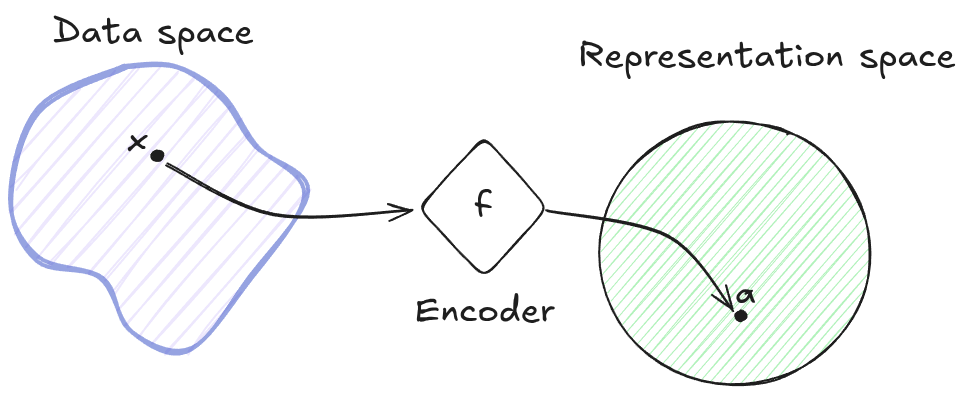
\includegraphics[width=0.75\textwidth]{images/Embeding.png}
    \caption[Embedding computations -- encode]{Embedding computations -- encode \cite{torralba_foundations_2024}}
    \label{fig:embedding}
\end{figure}

Representing data as an embedding vector creates a nice abstraction for computation. This abstraction enables computers to work with various formats in a unified manner, apply mathematical operations for processing, and, in some cases, facilitate a clearer understanding of those operations. A useful example is the indexing of such data in database systems. Having such a representation enables indexing of embeddings regardless of the data source's format.

The three main motivations for embeddings are the following:
\begin{itemize}
    \item \textbf{Compression} \\
    Embedding data can compress the original data (lossy or lossless). Such compression can reduce the storage requirements and the workload on systems that process embeddings, rather than on the original data sources.
    \item \textbf{Clearing out nuisance factors} \\
    Correctly processed information can remove data from the original source and factor out elements such as camera noise, lighting conditions, viewing angle, rotation, and others.
    \item \textbf{Decoupling} \\
    By combining the previous two features of representing raw data as embedding, it's possible to detect raw data that are either the same or hold the same information as others (according to the used model). Data projected to the same embedding can be grouped, enabling the deletion of duplicates and reducing storage and computational requirements.
    
    \cite{torralba_foundations_2024}
\end{itemize}

At the same time, embeddings entail important trade-offs. Since the mapping should also provide compression and is difficult to achieve without losing information, it must determine which factors of variation to preserve and which to discard for a given task. Different families of embeddings emphasize different visual cues and invariances, which is why various types of embeddings are suitable for a wide range of problems.

\section{Applications of Image Embeddings} \label{sec:applications_of_image_embeddings}
In the previous section, embedding is described as a process of representing data, but it is not clear which operations are suitable for such representations. One of the most well-known applications of embeddings is nearest-neighbor search. This use case employs embeddings (also known as autoencoders) to convert input data into a vector representation. Since vectors are mathematical objects on which relations such as distance can be defined and computed, those embeddings can be used to evaluate the distance between different data sources. Thanks to embedding, it is possible to define and compute distances between two sounds, images, videos, and other multimedia elements. This leads to various problems that can be addressed by understanding the distance between data sources, such as recommendation or search. The visualization of such an operation is illustrated in Figure \ref{fig:embedding_distance}.\cite{torralba_foundations_2024}
\begin{figure}[!ht]
    \centering
    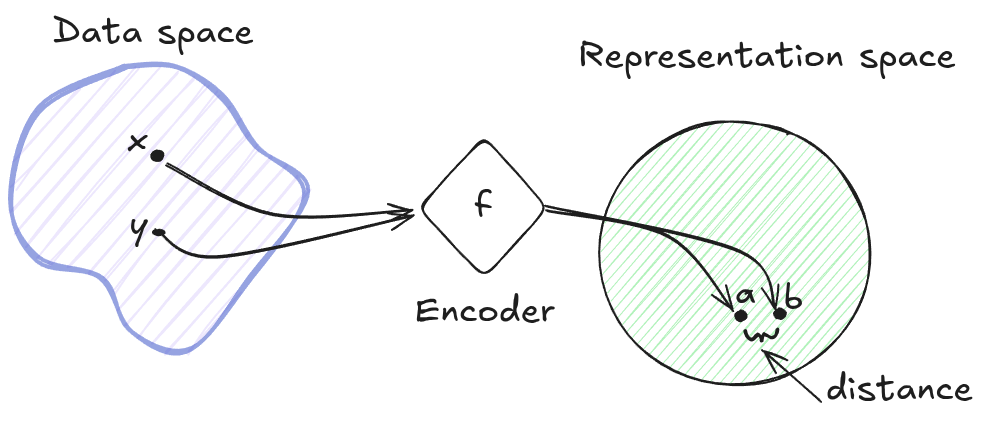
\includegraphics[width=0.75\textwidth]{images/Embeding_distance.png}
    \caption[Embedding computations -- distance]{Embedding computations -- distance \cite{torralba_foundations_2024}}
    \label{fig:embedding_distance}
\end{figure}

Another application of embeddings is predictive encoding. This is valuable for tasks such as object detection in image processing and for predicting missing data. Its use case is often seen in photo-manipulation programs, where it allows users to remove unwanted objects from the scene and replace them with elements that better fit the scene. \cite{torralba_foundations_2024}


\section{Models of Embedding Computations} \label{sec:offline_vs_online_processing}
Image-embedding systems are typically classified into two modes: online, in which embeddings are computed on demand per request, and offline, in which embeddings are precomputed and stored for later use. Both modes can coexist in real deployments, but they typically optimize very different constraints and failure risks. An example of coexistence, which also highlights the differences, is shown in Figure \ref{fig:online_offline_ec}. \cite{kiely_high-performance_2025}

\subsection{Online Processing} \label{sec:online_processing}
Online processing (also known as real-time processing) computes an image's embedding on request and returns the result with minimal additional latency. Latency is essential when the input is unknown in advance (e.g., when a user uploads an image for processing). The system must minimize queueing and cold-start effects, and enforce predictable latency, even under high traffic. To meet such requirements and optimize latency, any external dependency (e.g., remote fetches, model-weight loading) can degrade the user experience. Online pipelines, therefore, emphasize caching, admission control, and fast failure handling, accepting higher infrastructure cost to protect response times. \cite{kiely_high-performance_2025, liu_evaluation_2018}

\subsection{Offline Processing} \label{sec:offline_processing}
Offline processing (also known as batch processing) precomputes image embeddings and persists both input and output for later reuse. Images are ingested from references (typically URLs), validated as decodable media, normalized to a bounded resolution, and stored internally to eliminate reliance on unstable sources. Such computation saturates hardware efficiently and throttles as capacity dictates. The resulting vectors are linked to their source objects and model versions, enabling reproducible re-embedding when models evolve. Because offline jobs are not user-facing, the pipeline optimizes for throughput and durability rather than strict per-request latency. \cite{kiely_high-performance_2025, liu_evaluation_2018}
\begin{figure}[!ht]
    \centering
    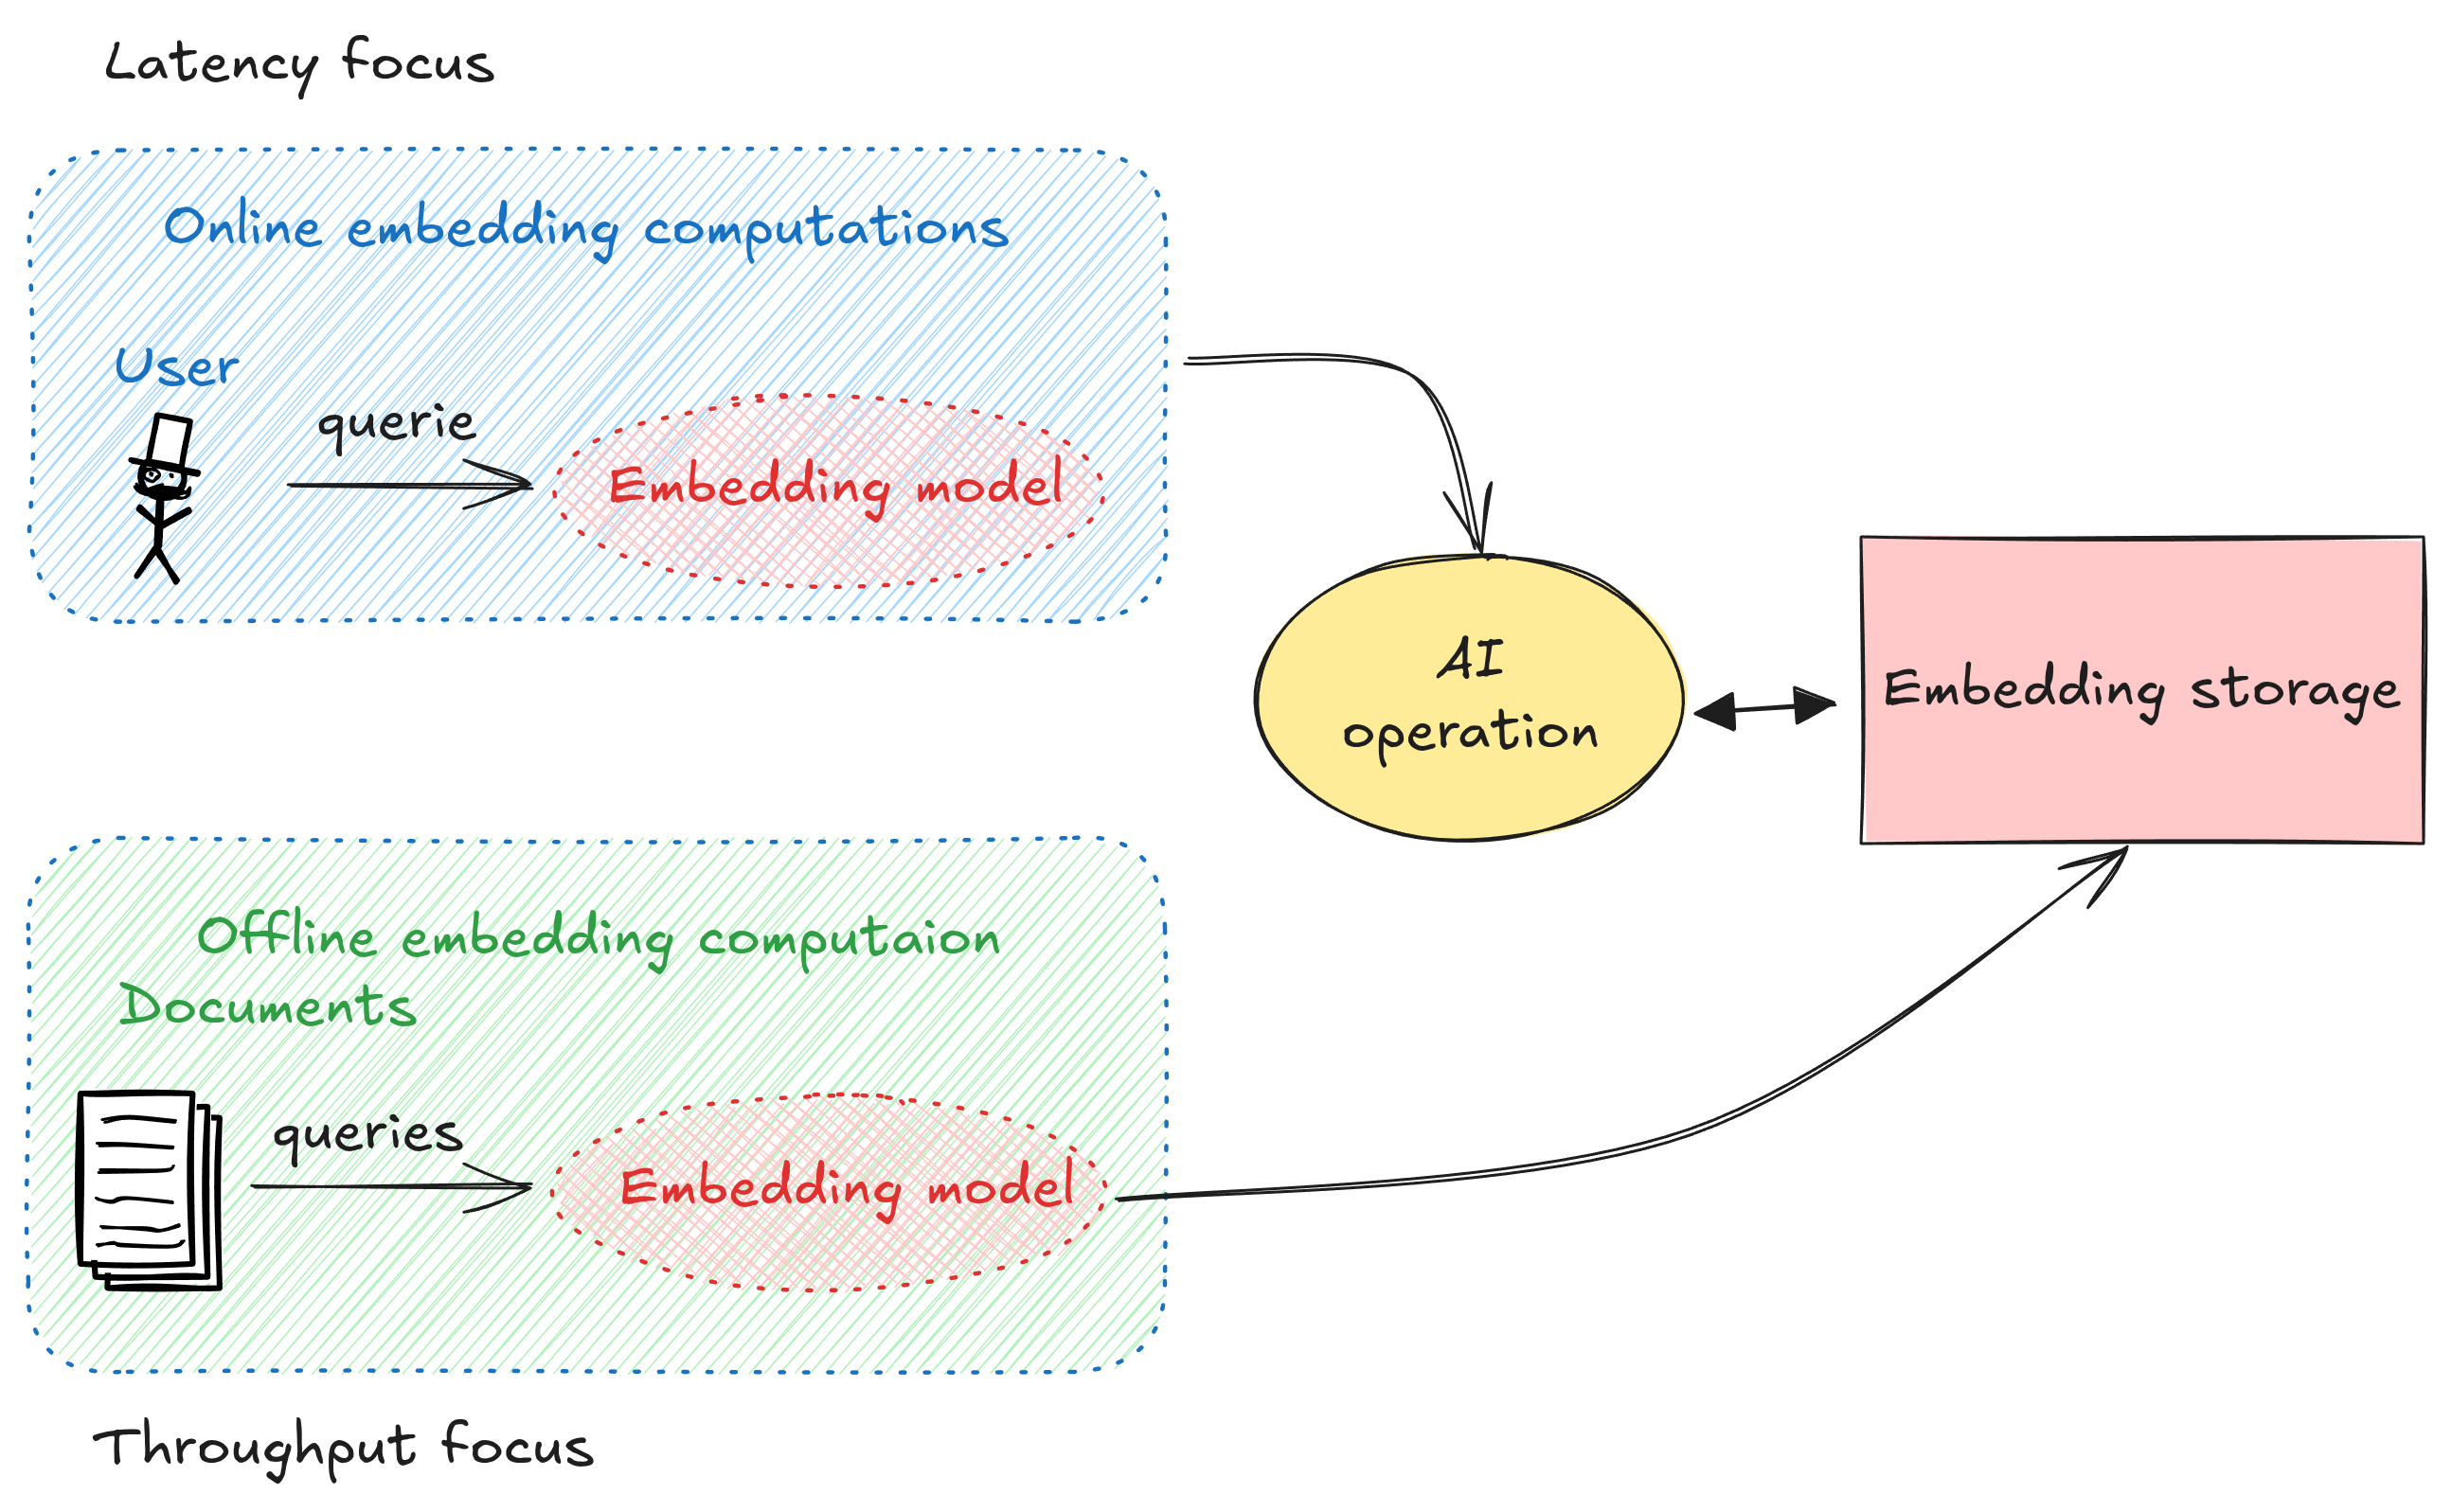
\includegraphics[width=0.75\textwidth]{images/Online_offline_ec.png}
    \caption[Online and offline embedding computation]{Online and offline embedding computation \cite{torralba_foundations_2024}}
    \label{fig:online_offline_ec}
\end{figure}

\vspace{1.5em}
Online and offline models of image processing are fundamental, often distinguished in theoretical discussions of image processing. Another model is stream processing, a hybrid of online and offline processing. It is a method that combines both throughput (from offline) and latency (from online). Such a system is the topic of this thesis. The problem of stream processing will be discussed in detail later in Chapter \ref{ch:data_processing}. For now, it is enough for the reader to be aware of the differences between online and offline processing.

\section{The Small File Problem} \label{sec:small_files_problem}
Systems that store images in the size range from $\approx 10$\,KiB to $1$\,MiB, at which this thesis is aimed, create a challenge known as the Small File Problem. This issue arises because traditional storage solutions, particularly file systems, were not designed to efficiently handle a large number of small, discrete files. The core of the problem lies in metadata overhead and file placement methods, which result in inefficiency in I/O.

Traditional file systems, such as POSIX, were designed for general-purpose single-machine use. They are tightly coupled to the operating system and store a significant amount of metadata for every file -- including permissions, ownership, timestamps (access, modification, change), and block pointers. For large files, these metadata are negligible; for small files such as images, the metadata (e.g., the inode and directory entries) can consume a disproportionately large amount of space and, more importantly, require a separate I/O operation to access.\cite{beaver_finding_2010}

This design leads to severe performance degradation at scale. To read one small file, the system must often perform multiple physical I/O operations: one or more to traverse the directory structure, another to read the file's inode (metadata), and a final one to read the actual data block. When processing millions of files, the storage subsystem is bottlenecked by these metadata-heavy random-access lookups rather than by sequential data reads. This high I/O overhead is unnecessary for ML applications, which often only need to identify a file by a unique key and retrieve its binary content. \cite{beaver_finding_2010}

\chapter{Theoretical Part -- Storage}\label{ch:storage_theory}
\section{Storage Abstractions}
Storage systems have evolved from simple, basic designs that meet basic criteria to modern systems intended to satisfy the needs of the modern computing era. This and the following sections will focus on explaining the basics of storage solutions, their evolution, and the emergence of the need for distributed storage. This should help the reader better understand how storage systems have evolved and highlight the needs that led to the creation of the software-defined storage principle.

Traditional storage solutions can be categorized into three main types (block storage, file systems, and object storage), each of which provides different needs with its own abstraction layer.

\subsection{Block Storage}
Block storage represents a foundational abstraction layer in modern computing and server architectures. It provides an abstraction layer for various physical storage systems, such as hard drives, solid-state drives, and storage networks. This abstraction allows a separation between the physical implementation of the underlying storage solution and the logical understanding of the provided storage. Consequently, this offers an easy communication interface between storage architects who deal with low-level solutions and infrastructure, and application architects who use that storage for their needs.

Block storage devices transform the storage layer into fixed-size logical blocks. These blocks are usually referenced via linear addressing, allowing applications to access precise parts of the devices. This allows almost complete access to the logical storage provided by the low-level architecture. This type of access does not limit applications or users in any way. The user of the block device is usually expected to manage and organize the data in the underlying storage themselves.

Direct use of block storage is often preferred for IO performance-sensitive applications, since it allows direct access to storage, and the organization of data can be tuned in any form that suits the application's needs.

Databases such as Oracle, Aerospike, and others use direct access to block storage devices. This allows those systems to manage their data structures directly. This can lead to optimizing memory operations by correctly serializing data in storage and implementing logic directly on the device. \cite{oracle_storing_2025, aerospike_ssd_2024} 

Direct access to block storage often requires complex implementation and requires a deep understanding of low-level concepts. However, specifically designed storage for specific use cases can lead to optimized storage access.

Although specialized applications use it directly, block storage is more commonly used as a building block for higher-level storage layers and abstractions. One such abstraction is a file system, which maps blocks of memory to files, directories, and other structures.\cite{muzikar_zarizeni_2025}

\subsection{File Systems}
The most common and well-known storage abstraction built on top of block devices is a file system. This abstraction layer introduces a familiar hierarchical structure of files and directories (or folders). Data are encapsulated in files (as logical units of data) and subsequently organized within a nested directory structure. A specific file is addressed using a path that defines a unique route through this hierarchy. Even though most users intuitively understand this model, its underlying implementation is significantly more complex than other storage abstractions, such as object storage.

This abstraction is comfortable because it shields the user and the application from the physical complexities of data storage. Instead of interacting with raw block addresses, the system interacts with logical files. The implementation of a file system is responsible for managing all low-level complexities, such as the placement of physical data and block allocation. This file-level and directory-level structure also simplifies higher-level operations, such as backups and replication, since these can be performed directly on the logical constructs (folders and files). \cite{muzikar_systemy_2025}

Another nice feature of file systems is native support for metadata. In most common file system implementations (POSIX-based), each file and directory maintains a set of metadata, which typically includes ownership (user, group), access permissions, timestamps (access, modification, change), and block pointers. For a large file, this metadata is negligible; however, for small files like images, the metadata (e.g., the inode and directory entries) can consume a large amount of space and, more importantly, a separate I/O operation to access.\cite{beaver_finding_2010}

It may seem that abstracting storage into files and folders is a clever and intuitive way to structure data, but such a solution also has drawbacks regarding performance and scalability. The first major drawback is the latency introduced by hierarchical path-based addressing. To read a single file, the file system must walk the entire path from the root \cite{beaver_finding_2010}. In common implementations, the (so-called) walk process involves accessing multiple structures stored on disk to finally access the needed data. In the case of XFS, the system must traverse the hierarchy, like in the following example:
\begin{quote}
\texttt{/}\\
\texttt{/folder/}\\
\texttt{/folder/subfolder/}\\
\texttt{/folder/subfolder/data.file}
\end{quote}
Such a walk often generates significant metadata overhead and I/O operations that are (in most cases) not needed by applications operating on the storage system.\footnote{Modern systems heavily rely on cache; Walk overhead is present only in cold cache systems or non-systematically accessing a large amount of files. This thesis addresses the problem of large amounts of data, so the walk issue remains valid.} \cite{beaver_finding_2010}

Another significant drawback of file systems is that they are designed for isolated single-node environments. To guarantee consistency of its internal structures and prevent data corruption due to race conditions, the file system must rely heavily on locking. This mechanism often forces the serialization of many operations. This serialization occurs when writing to the same file, modifying the same directory, or concurrently modifying the metadata \cite{yuan_introduction_2020}. Although it is not necessarily a problem in non-shared storage solutions and personal systems, the latency caused by locking may be significant in shared file systems on the network, where locks must be performed over the network. This may lead to weak performance in distributed solutions. \cite{liu_evaluation_2018}

\subsection{Object Storage}
Object storage is a relatively simple abstraction for managing data at scale. Its fundamental unit is the object. An object is a self-contained entity that contains raw data, descriptive metadata, and a unique identifier. Objects are organized in a flat namespace (known as buckets or collections) as an unordered set. Each object in a collection has a unique identifier by which it can be addressed. Some implementations may simulate hierarchical structures by embedding slashes in object names; however, from a design perspective, the namespace remains logically flat and no hierarchy is applied. \cite{mesnier_storage_2003}

Data are stored as raw binary data (the object's content) on the underlying storage systems. The data for one object are atomic and treated as a single data chunk. That makes operations with objects simple, such as writing or reading the whole object -- updates of some part of the data are typically not allowed. \cite{mesnier_storage_2003}

Having a unique key that addresses raw data essentially forms storage systems that can be treated as simple key-value stores.

The core component that realizes this abstraction is the object store. The object store is a service that orchestrates storage and maps object names, their metadata, and their physical locations. It can be considered as a database engine that implements the described key-value storage. The object store is responsible for maintaining the mapping between object identifiers and their physical placement, orchestrating data and metadata operations between storage nodes, and enforcing consistency, durability, and access policies. \cite{mesnier_storage_2003}

Object storage is a simple abstraction that enables higher-level use cases for users and applications. At its core, it has just three simple rules.
\begin{itemize}
    \item \textbf{Atomicity of an object} \\
    Each object is atomic and treated as an indivisible unit of data. The only supported operations are write, read, and delete of the whole objects. The data inside the object can be any binary data of any size or length (blob).
    \item \textbf{Unique Identifier} \\
    Every object is associated with a unique identifier (key) within its namespace, which is used to address it. This key abstracts away the physical location of the data and enables simple key-value-style operations for clients.
    \item \textbf{Object store as an orchestration} \\
    The object store is a service that manages the global namespace, metadata, and placement of objects across storage nodes. It orchestrates data and metadata operations, enforces consistency, durability, and access policies, and abstracts key values on top of the underlying storage resources.\\
\cite{mesnier_storage_2003}
\end{itemize}

One of the biggest advantages of object storage is that it provides a highly scalable, durable, and performant solution compared to traditional file and block storage. Its primary strength is massive scalability and high throughput. The flat namespace and decoupled metadata allow the system to scale horizontally across multiple nodes, leading to better quality of service. Its ability to scale to remote nodes enables data replication, erasure coding, and self-healing to ensure high durability and fault tolerance. \cite{systemdesignschool_maximizing_2025}

Another key feature of object storage is its access interface. Instead of using local file system protocols, object storage is typically accessed via network-based APIs or protocols, with Amazon S3 being the most well-known example. This network-centric design decouples the storage system from any specific operating system, which simplifies integration in distributed environments.

Despite these advantages, object storage abstraction introduces some fundamental limitations. The most significant aspect is data immutability and atomicity. Unlike files on a POSIX system, objects cannot be modified in-place. Since objects are atomic, any update requires loading the entire object into memory, modifying it, and then updating it. This operational model is highly inefficient for granular updates and transactional workloads.

Another trade-off in achieving massive scalability and high availability is that many distributed object stores often sacrifice strong consistency in favor of eventual consistency. In practice, this means that a successful write operation may not be immediately visible to all subsequent read requests, which can be problematic for applications that require strict read-after-write consistency.

Finally, since object storage systems usually do not provide a native POSIX interface, this can be a significant barrier for legacy applications. While there are often compatibility layers or gateways that expose a POSIX-like interface on top of object storage, these typically introduce performance and reliability issues because they must translate between two fundamentally different abstractions. \cite{mesnier_storage_2003, systemdesignschool_maximizing_2025}

\vspace{1.5em}
Both file systems and object storage are built on the same underlying block-based hardware and represent two different ways of thinking about data. Object storage treats data as self-contained objects addressed by identifiers in a flat namespace, which shifts the focus from navigating directory trees to operating on independent blobs via a simple key-value system. It is important to note that object storage does not introduce a fundamentally new storage technology at the physical layer -- the data are still stored on block devices or similar media. The main innovation lies in the interface, how data are named, grouped, and accessed over the network, rather than how bits are laid out and retrieved from the physical storage devices themselves. To better understand the interface, see Figure \ref{fig:object_storage_vs_fs}.

\begin{figure}[!ht]
    \centering
    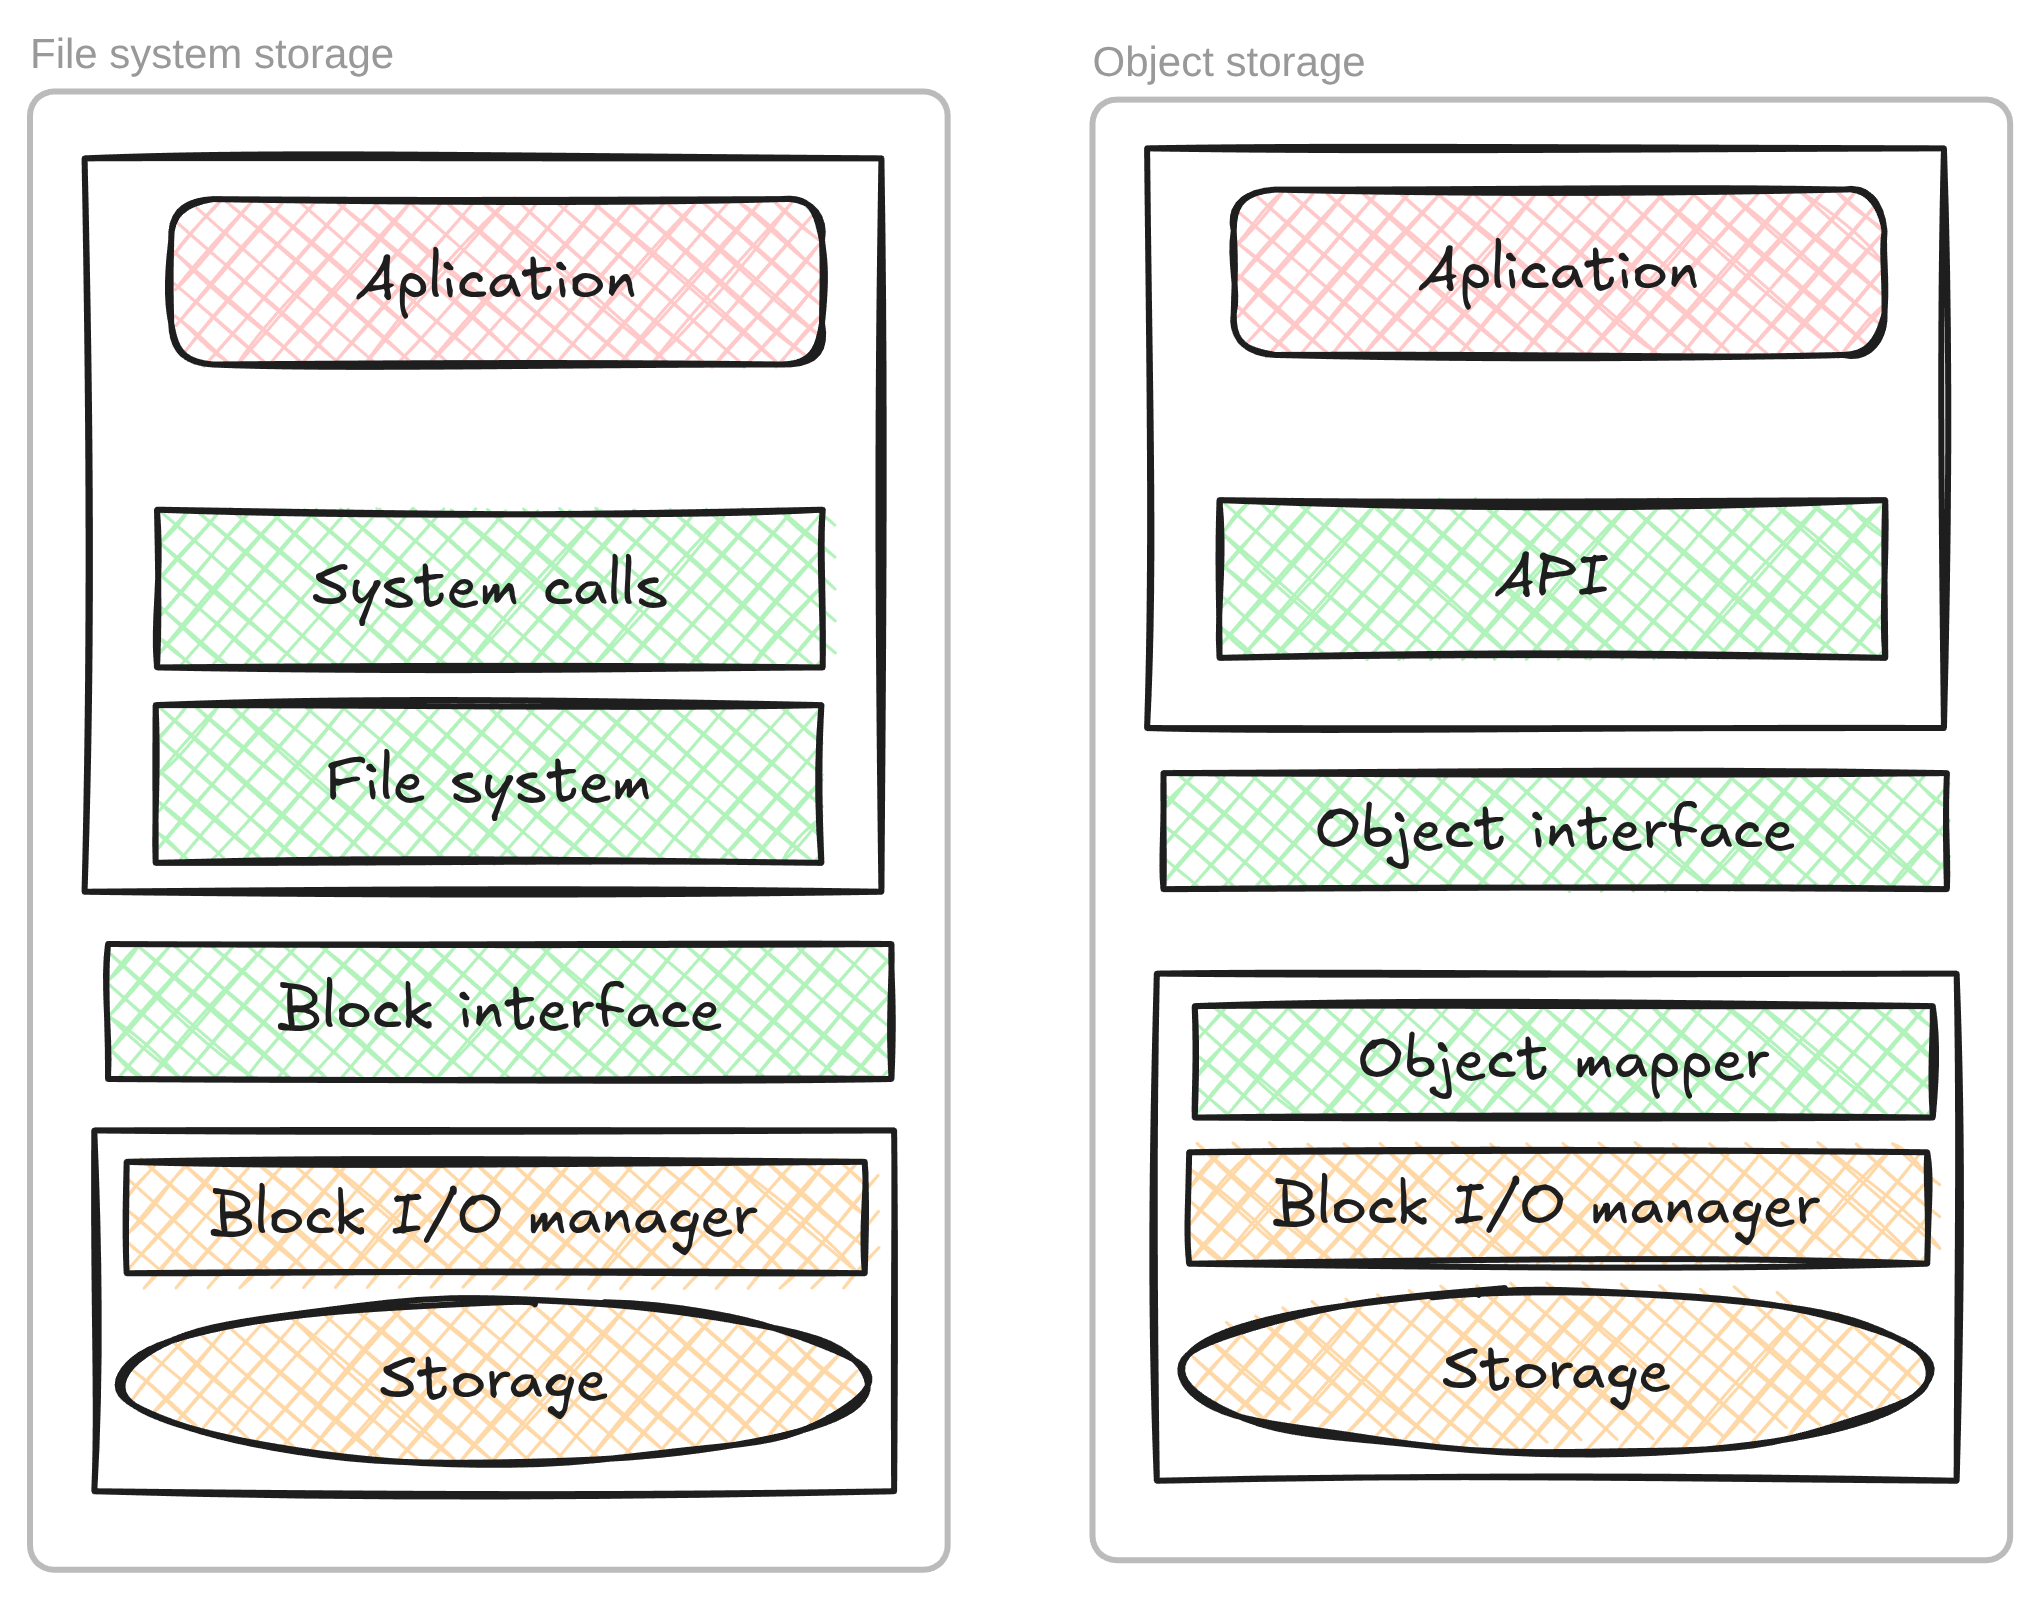
\includegraphics[width=0.9\textwidth]{images/object.png}
    \caption[Comparison  of storage interfaces]{
        \label{fig:object_storage_vs_fs}
        Storage interfaces for file systems and object storage solutions
        \cite{mesnier_storage_2003}
        }
\end{figure}

\vspace{1.5em}
The previous sections outlined three common abstraction layers and design patterns for storage systems. These abstractions remain fundamental to modern computing, and all following storage systems build on top of them.

\section{Software-Defined Storage}\label{ch:sds}
As many other fields in computer science (by both academic research and industrial needs) have evolved into new solutions, so has the storage subsystem. One of the directions storage subsystems went is towards distributed storage systems (its motivations and architecture will be discussed in the following chapters). Contemporary distributed storage solutions are frequently built within the broader framework of software-defined systems, specifically software-defined storage (SDStorage).

The software-defined system (SDSys) paradigm is a significant architectural shift whose main idea is to implement, through software, the management and control of underlying physical infrastructure. Such systems typically leverage existing hardware as a substrate, upon which software layers provide extended functionality and policy-driven behavior. \cite{moucha_software_2021, darabseh_sdstorage_2015}.

A core goal of any SDSys is to hide the complexity of resource management and control from end users \cite{darabseh_sdstorage_2015}. By moving resources to service-like abstractions, SDSys enables a clear expression of requirements (e.g., QoS levels, placement policies), consistent and system-wide enforcement of policies \cite{darabseh_sdstorage_2015, moucha_software_2021}. The first widely adopted realization of this idea appeared in networking as software-defined networking (SDN). Later, an experimental framework called SDStorage was introduced in an article presented by Staffordshire, IBM Corporation, and other co-authors, taking inspiration from the implementation of SDN (concretely Mininet Software) \cite{darabseh_sdstorage_2015}. The authors of the article mention that the SDN technology helped them create the foundation of SDStorage.

\subsection{SDStorage Architecture}
From a higher-level perspective, software-defined storage is typically split into two planes: a control plane and a data plane. The control plane provides the system’s intelligence. It maintains a global view of resources, translates API requests into executable rules and actions, orchestrates placement, controls replication, and monitors health and performance. The data plane executes those rules along with the I/O operations on the underlying physical storage system, serving as a data layer for the control plane. It performs the actual read/write operations. The control plane uses the data plane to enforce the policy (e.g., caching, compression, encryption, replication\ldots). This separation reduces complexity, improves modularity, and enables consistent policy-driven behavior across heterogeneous hardware. \cite{moucha_software_2021}

\begin{itemize}
    \item \textbf{Control Plane} \\
    The control plane is the core of an SDStorage architecture, providing the system’s intelligence and acting as its coordinating brain. It is typically implemented as a logically centralized controller that coordinates, manages, and enforces policies throughout the storage environment. Its primary functions include provisioning and orchestrating volumes, automating lifecycle operations, maintaining a global view of resources and state, and translating user-defined (business-level) policies into concrete executable instructions. Through the control plane, SDStorage platforms enforce QoS and other policy requirements consistently across heterogeneous backend (physical storage). \cite{darabseh_sdstorage_2015, macedo_survey_2021, faisal_software-defined_2024}
    \item \textbf{Data Plane} \\
    The data plane is where the storage service is realized -- it executes I/O against underlying physical storage. It is responsible for performance, durability, and efficiency. It is a component available to the control plane that enforces controller-defined policies over data. Among typical I/O functionality, it may be responsible for replication, compression, deduplication, and caching. Within SDStorage, the data plane corresponds to the underlying storage infrastructure and assets on which these operations are performed. \cite{darabseh_sdstorage_2015, macedo_survey_2021, faisal_software-defined_2024} \\
    Its main role is to abstract the underlying hardware storage (e.g., block and file systems) and provide it to the control plane as unified storage.
\end{itemize} 

The last component, not often mentioned in the SDStorage system, is the management layer. This component is usually responsible for organizing and managing the entire system and interacts with the control plane. It can be used to describe management tools (such as web user interfaces) to administer such systems \cite{kohli_next_2022, moucha_software_2021}. Since it is rarely explicitly discussed and often merged into the control plane, only data and control planes will be discussed in the thesis.

Together, the control plane and the data plane form a complete storage system capable of providing core storage functionality. The schema of such systems, with the corresponding responsibilities, is shown in figure \ref{fig:architecture_of_distributed_solutions}\footnote{Figure shows all three components (control, management, and data plane). Control and management planes are often merged into one component.}.

\begin{figure}[!ht]
    \centering
    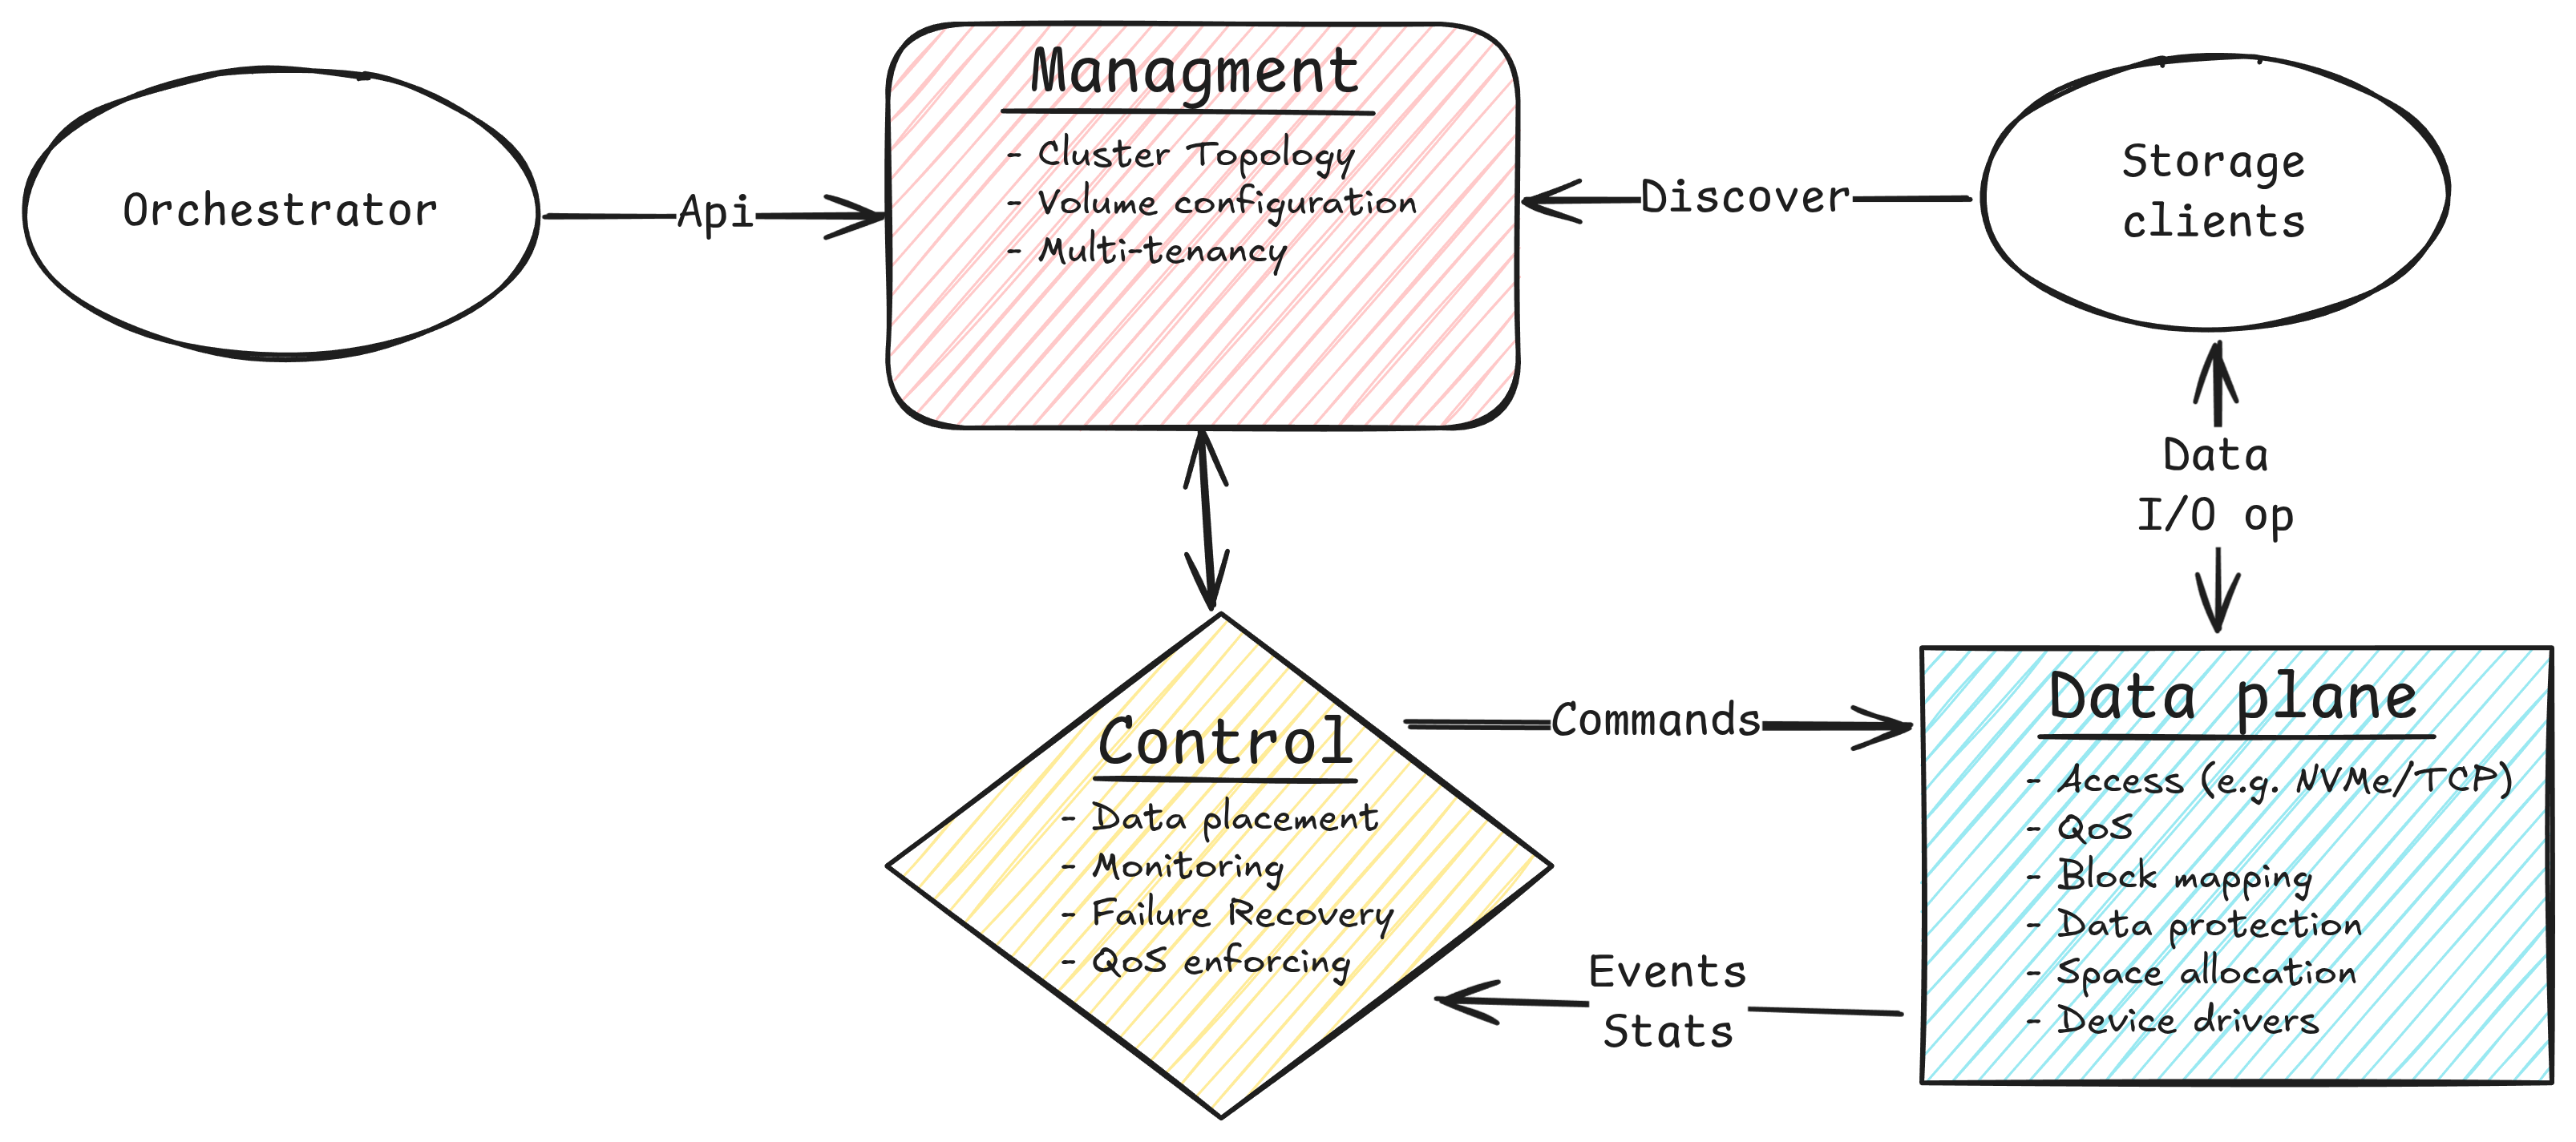
\includegraphics[width=0.9\textwidth]{images/architecture_of_distributed_solutions.png}
    \caption[Architecture of SDStorage]{
        \label{fig:architecture_of_distributed_solutions}
        Architecture of SDStorage\cite{kohli_next_2022}
        }
\end{figure}

\subsection{Interfaces on SDStorages}
Traditional storage provides an interface via the systemcalls implemented by the underlying operating system. In SDStorage, the control plane serves as the primary entry point for users and applications, offering explicit application interfaces (APIs) to interface with storage. This is the main difference between traditional systems. As in object storage (Figure \ref{fig:object_storage_vs_fs}), the SDStorage interface is a general API that offers greater control. This allows users to define any type of API suitable for the needs of a concrete storage system and its application needs.

By decoupling the data plane and control plane and freeing the storage stack from dependencies on a rigid interface, SDStorage makes the storage stack more flexible and extensible. It can compose new services, evolve semantics (e.g., tiering, encryption, erasure coding). It also enables modifying storage for specific needs without large changes to the API \cite{darabseh_sdstorage_2015}.

\subsection{Advantages of SDStorage}
Treating the storage system as software brings several benefits by rethinking the schema in a software-oriented way. The following are some advantages of using SDStorage:

\begin{itemize}
    \item \textbf{Removes Hardware Dependency} \\
    Software-defined systems (in general) decouple functionality from underlying hardware. This enables organizations to deploy applications on mixed-vendor infrastructure. Hardware independence reduces dependence on specialized appliances and vendor lock-in. This leads to a more flexible deployment environment and may reduce the overall system cost. \cite{faisal_software-defined_2024}
    
    \item \textbf{Performance Scalability} \\
    The architecture design of SDSys brings scale-out nature even to SDStorage systems. Storage resources can be expanded horizontally by adding new data nodes, without disruptive architectural changes. This allows capacity and I/O performance to grow and scale out. Some solutions claim even the possibility to scale out linearly (when pre-requisistes) are met. \cite{parkes_cephio_2025}

    In addition to data scalability, the software way of thinking allows easy implementation of cache subsystems at any specific abstraction level. This allows tuning performance for specific needs. It is suited for high-performance environments with the possibility of tuning parameters such as latency, file sizes, and consistency \cite{faisal_software-defined_2024}.
    
    \item \textbf{Operations, Automation, and IaC} \\
    SDSys replaces device-centric management with a centralized control plane that controls heterogeneous resources. Administrators can manage diverse pools of infrastructure from a single logical point, using uniform policies instead of device-specific configuration. This unification significantly reduces operational complexity and human error.

    By introducing the management plane, the operations of storage systems can be easily abstracted by policies and other concepts. Provisioning, data placement, replication, backup, and lifecycle operations are expressed as high-level policies and executed automatically by the control plane.
    
     API-driven programmability makes infrastructure fully scriptable and allows use of Infrastructure-as-Code practices. \cite{faisal_software-defined_2024}
    \item \textbf{Data and Resource Management} \\
    SDStorage introduces a unified approach to managing heterogeneous storage resources without limiting their specific usage. By providing a unified view across block, file, and object storage, it enables consistent monitoring, policy enforcement, and capacity planning across diverse media types. \cite{faisal_software-defined_2024}

\end{itemize}



\section{Distributed Storage Solutions}\label{sec:distributed_solutions}
The previous Chapter \ref{ch:sds} has highlighted that software-defined storage solutions have a crucial role in designing distributed storage solutions. Distributed storage solutions represent another approach to address the continuously evolving needs of storage systems.

Modern computing environments face significant challenges in managing the growing volume of data. Traditional storage solutions often struggle to meet the scalability, fault tolerance, and high-performance requirements of modern applications. The rise of cloud computing has amplified these challenges, as dynamic workloads and distributed applications demand storage solutions that can adapt and scale efficiently. Another part of computation that introduces new challenges for storage systems is grid computing, in which parallel access to storage is required. \cite{langr_paralelni_2024}

The concept of distributed storage solutions has emerged to address these issues. A distributed storage solution can represent various solutions or their combination. To clarify the solutions, here is a list with explanations.

\begin{itemize}
    \item \textbf{Parallel File and Object Writing} \\
    Traditional file systems and object stores do not allow parallel writes to the same file or object at the same time. When two subjects attempt to access (write) the data simultaneously, they must synchronize their access. This can be a problem in HPC, when data are usually enormous and computational power is time-limited. Distributed storage solutions address this by enabling parallel writes to different data nodes in a cluster. \cite{langr_paralelni_2024}
    \item \textbf{Replicated Storage} \\
    Replicated storage ensures data redundancy by storing multiple copies of the same data across different nodes in a distributed system. This improves data reliability and availability. If one node fails, the system can seamlessly access data from another replica. Replication can be synchronous (immediate replication to all nodes) or asynchronous (updates occur after a delay). Common use cases include disaster recovery, fault tolerance, and read-intensive workloads, in which replicas distribute the read load. \cite{tudelft_225_2023}
    \item \textbf{Remote Storage} \\
    Remote storage allows data to be stored on a different physical or virtual location and accessed over a network. It decouples storage from compute resources, enabling greater flexibility in resource allocation. Network protocols such as NFS (Network File System) or iSCSI (Internet Small Computer Systems Interface) facilitate access to remote storage. This approach is often used in cloud environments and distributed systems where centralized data storage is necessary. \cite{vondra_storage_2022}
    \item \textbf{Remote Storage Pools} \\
    Remote storage pools aggregate multiple remote storage resources into a single logical pool. This abstraction allows users to manage and utilize storage more efficiently without worrying about the underlying physical location of the data. Storage pools can span multiple nodes, data centers, or even cloud regions, offering seamless scalability, load balancing, and high availability. This is particularly useful in hybrid and multi-cloud setups. \cite{vondra_storage_2022}
\end{itemize}

\vspace{1.5em}
From now on, this thesis will mainly discuss remote storage pools. When addressing distributed storage, consider a solution that can serve remote storage pools. This chapter will focus on the scalability of those storage systems, their replication, fault tolerance, performance, and the APIs they offer to users. Other types of distributed storage are not relevant to this topic.

\subsection{Architecture of Distributed Storages}
The architecture of modern distributed storage solutions is highly dependent on the principles of Software-Defined Storage established in Chapter \ref{ch:sds}. While traditional storage architectures tightly bind data to specific hardware controllers, distributed solutions leverage SDS decoupling of the control and data planes to offer storage that spans multiple servers (nodes), creating a unified system.

In a distributed SDStorage architecture, the control plane usually maintains a map of the cluster (set of nodes) and controls the data plane on each node. It uses the raw storage capacity provided by the data plane's individual nodes into a shared, logical construct often referred to as a Storage Pool.

Instead of interacting with physical disks, the control plane abstracts these resources. It treats the collection of all underlying drives in the network as a single contiguous storage space. This architecture extends the SDStorage's features to distributed systems and adds several others. The key ones are:

\begin{itemize}
    \item \textbf{Global Resource Management}  \\
    The control plane maintains the global state of the storage cluster. It usually monitors the total available capacity and health of the pool, and the state of the data node. This makes it easier to maintain a storage pool as a single coherent system rather than managing individual nodes in isolation.
    \item \textbf{Dynamic Scalability} \\
    Data nodes in distributed storage systems are treated as "worker" nodes, controlled by the master (control plane). Data planes can be independent of each other, since they just serve resources to the control plane. This allows easy dynamic scaling. When a new node is added to the cluster, the control plane detects the new data plane resources and automatically adds them to the storage pool, increasing the total capacity without service interruption.
    \item \textbf{Policy-Based Distribution} \\
    In a distributed environment, data placement and resource allocation are controlled by the control plane. This allows organizing data by logical definitions rather than hardware ones. This adds the possibility of implementing various data placement optimizations for any required use cases.  This enables the enforcement of Quality of Service rules. An example of QoS could be fault tolerance or throughput limits.
\end{itemize}
\cite{mark_carlson_software_2015, macedo_survey_2021, moucha_software_2021}

% TODO refraze
Another key advantage of distributed storage solutions is the ability to load-balance client requests across multiple data planes. Because data are typically replicated across several nodes, the system can direct read requests to any node that currently holds the requested data. This improves throughput and increases resilience to transient performance degradation of individual nodes. The concrete mechanisms for request distribution depend heavily on the particular implementation; therefore, it will be discussed for each storage system as it is introduced in the following text. \cite{macedo_survey_2021, moucha_software_2021}

\vspace{1.5em}

By combining the capabilities of software-defined storage and applying them to distributed storage systems, it's possible to create storage systems composed of multiple nodes that form a storage pool. With decoupling data storage layer and control layer, it is potential to build storage suitable for various needs. 

Once physical resources are aggregated into a pool, the system can carve out logical units for consumption, whether as block devices (volumes), file systems, or objects collections. Users and applications then interact only with needed logical units, while the system fully abstracts away the physical layout of the data. This architecture directly fulfills the main requirement of \emph{remote storage pools} discussed in the previous section. \cite{macedo_survey_2021, moucha_software_2021}

This architecture offers a wide range of possibilities when designing storage systems with defined QoS, based on their needs. The above-listed advantages come with trade-offs and problems that those systems need to address, the most common of which are data durability, consistency, and trade-offs among consistency, availability, and failure resilience.


\subsubsection{Data Durability}
Data durability describes the ability of a storage system to store data in a way that is resilient even for partial failures. In distributed storage, durability is primarily about ensuring that the data can survive hardware failures, software bugs, and operational mistakes without permanent loss. Because modern systems store large volumes of data on commodity hardware and across many nodes, failures are expected rather than exceptional, and durability mechanisms become a core part of system design.

In practice, durability is achieved by introducing redundancy and recovery plans. Two common approaches can be distinguished by their recovery characteristics. The first approach is backup, which typically provides durable copies at a lower operational cost but with slower recovery. The second approach provides fast recovery through online redundancy, such as replication or sharding combined with redundancy, in which the system can continue serving data even when some components fail and automatically rebuild missing replicas/shards.

This text will focus on online redundancy, since it's specified as one of requirements for solving problem described in the beginning of the thesis.  
\paragraph{Replication} \mbox{} \\
One way to ensure data durability is to replicate the data. That means keeping a full copy of the data on multiple nodes. This is one of the easiest and most intuitive ways to implement data durability. By maintaining data replicated on various nodes, it is guaranteed that no data will be lost in any case of failure in which at least one copy of the remaining data is available. The advantages of replication are its simplicity, which makes it easy to design recovery plans in case of any failure and partial (copy) data loss. Creating a copy of the data and replicating it across multiple availability zones also introduces the possibility of load-balancing read requests across data locations.\cite{kleppmann_designing_2017, liu_evaluation_2018}

An example of a replication solution is the Distributed Replicated Storage System (DRBD). DRBD is an open-source solution for block replication over the network between multiple Linux storage nodes. Linbit developed it, now DRBD is one of the most common solutions for block replication across Linux servers. Although there are other solutions, DRBD is one of the most used. It is mentioned here as a concrete implementation.

DRBD is implemented as a kernel module in a Linux kernel. It enables reliable replication (RAID 1) for Linux nodes across a network. This replication is often used to meet requirements for fault tolerance and high availability systems. Thanks to the replication, when all nodes but one are unavailable, the remaining one can still offer a fail-over and serve its purpose. This replication comes with a network usage cost and more storage space consumption from the storage pool. \cite{linbit_drbd9_2025}

Even though DRBD itself does not implement a distributed storage system (storage pool based) it's often used as a part of solutions to those systems as you will see in Section \ref{sec:linstore}

\paragraph{Partitioning} \mbox{} \\
Another approach used for data durability and fault tolerance in distributed storage is \emph{partitioning}. Partitioning (also called \emph{sharding}) splits the stored object into multiple smaller pieces (partitions) and distributes them across different nodes in a storage pool. By itself, partitioning mainly changes placement of the data. To add data durability it is often combined with additional redundant information to offer failure recovery (e.g., parity data), such data enables recovery in case of failure. In such a design, the system stores only a subset of redundant fragments instead of a full copy, so data can remain readable and recoverable even after a node outage. \cite{purestorage_what_2025}

This method is much more space-efficient than replication since it does not have to store full replication data. The disadvantage of this approach is a performance cost when data are being restored or written since partitions need to be recalculated. \cite{purestorage_what_2025} This type of durability mechanism is often better for cold data, which is not often accessed and modified.

In storage systems, the mechanism that turns partitioning into a durability method is commonly \emph{erasure coding}. Erasure coding encodes data into $k$ data fragments plus $m$ parity fragments (often marked as a $(k+m)$ scheme), distributed across different nodes. Such system allows data to be reconstructed from \emph{any} $k$ out of the $(k+m)$ fragments. This provides fault tolerance with substantially lower storage overhead than full replication, at the cost of additional computation during writes and recovery. \cite{simplyblock_authors_erasure_2026} To better understand mechanism of erasure coding, see Figure \ref{fig:ec}.
% TODo show n picture
\begin{figure}[h!t]
    \centering
    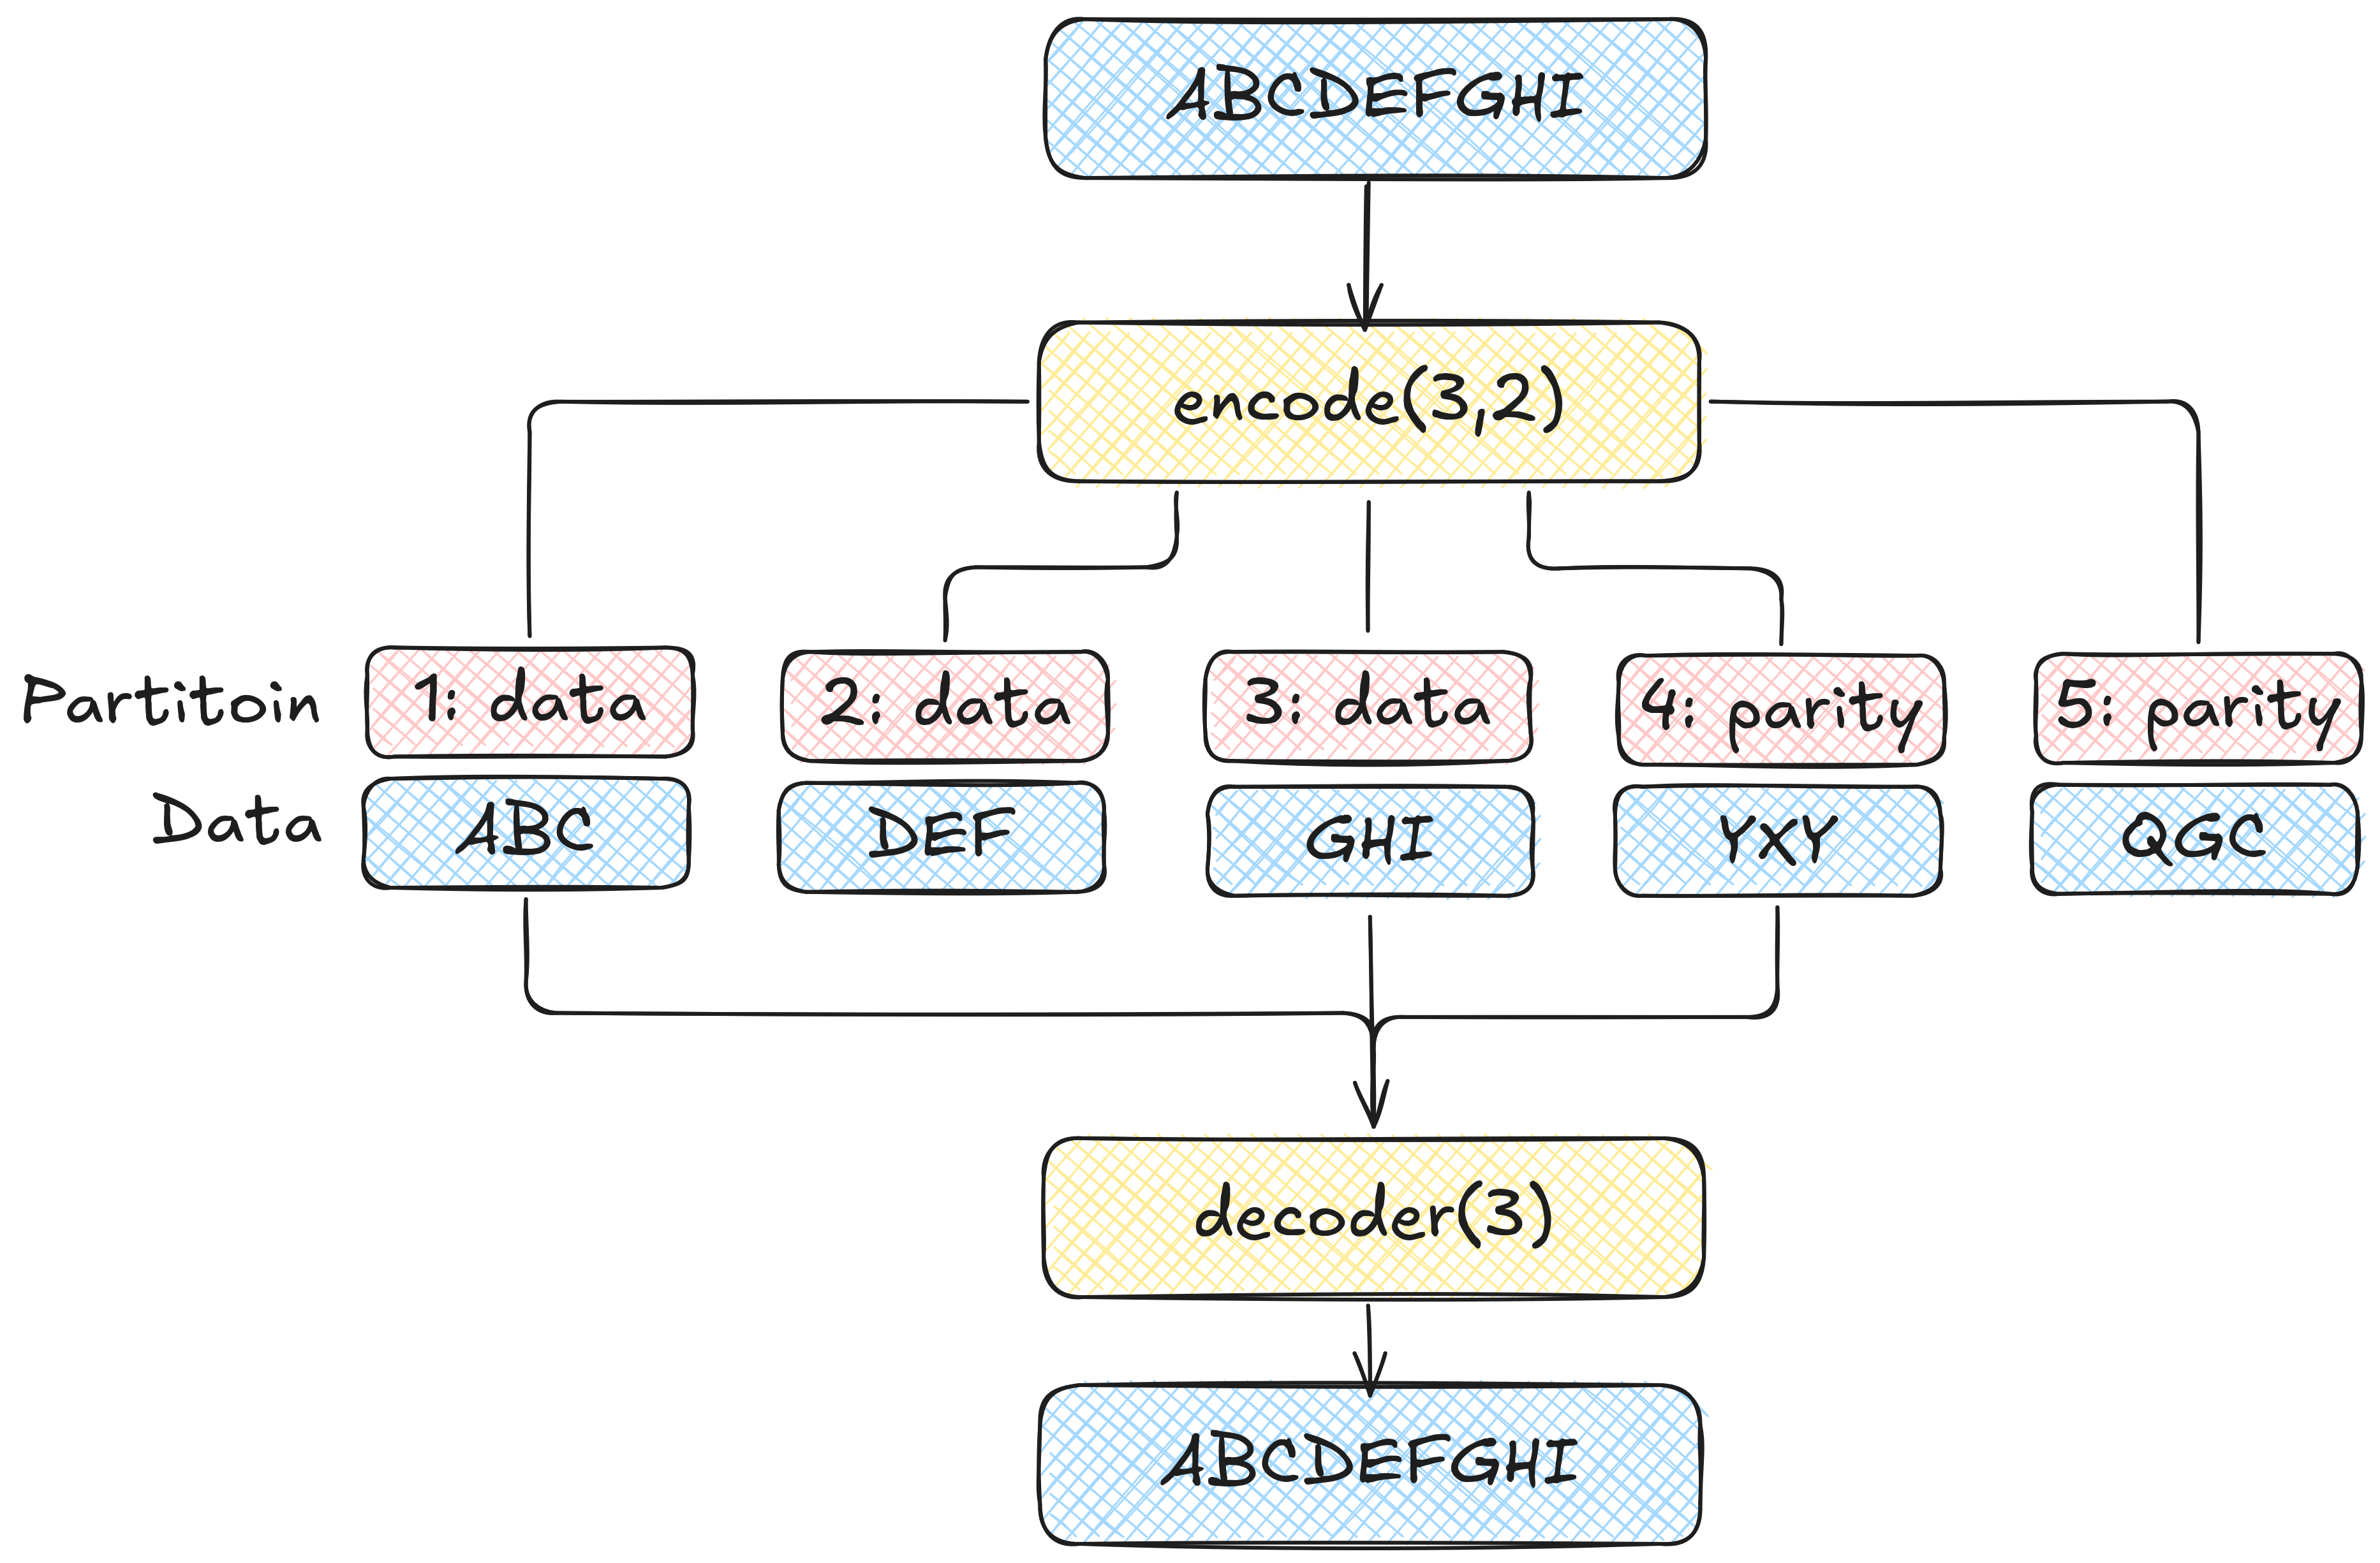
\includegraphics[width=0.9\textwidth]{images/ec.png}
    \caption[Erasure-coding schema]{\label{fig:ec}Erasure-coding schema -- $(3, 2)$\cite{ceph_authors_erasure_2016}}
\end{figure}
\vspace{1.5em}

% TODO the partitionng is often combined with replicatoin
\subsubsection{Consistency}
Introducing distributed systems that care about data durability, high availability, etc., always comes with shared data or knowledge of the system. Such systems must ensure the consistency of shared data. In a distributed system that contains data shared among servers, all nodes have a unique view of the data. It is critical to ensure that data stored on a distributed system remain accurate and coherent across all nodes. In storage systems, there are two main consistency patterns that describe how consistent the data are in a distributed system.\cite{geeksforgeeks_consistency_2025}

\begin{itemize}
    \item \textbf{Strong Consistency} \\
    \enquote{\textit{Ensures that all nodes in the system have the most up-to-date data at all times, with no lag or inconsistency between replicas.}}\cite{geeksforgeeks_consistency_2025}
    \item \textbf{Eventual Consistency} \\
    \enquote{\textit{Allows for temporary inconsistencies between replicas but guarantees that they will eventually converge to a consistent state without intervention.}}\cite{geeksforgeeks_consistency_2025}
\end{itemize}

Consistency levels are an important property of any distributed system that contains data for several reasons. Since distributed solutions are designed to enable scalability and prevent failures such as node outages, it is important to specify what happens in the event of data loss. Consistency patterns describe how systems behave in adverse scenarios and which states can or cannot guarantee correct data integrity. Among data integrity consistency patterns, ensuring quality of service of distributed solutions may offer better performance optimizations.

There are many types of consistency, which typically lie between two main types. First one is eventual consistency.
It requires that any comparable events must be performed in ordered, meaning that any event that directly or indirectly operates on the same data must be evaluated in the same order on every node. This type of consistency ensures that events can depend on one another and are executed correctly (an object's modification will be performed only after it is created). This pattern ensures that the sequence of (correct) operations on data in a distributed system will be correctly executed on every node. \cite{kleppmann_designing_2017} Such ordering implies that the system will eventually reach full consistency for each operation. This means that for each operation, there exists (or will exist) a time at which this operation was performed on all available nodes in the distributed system, and at that point, all systems had a consistent set of data. This ensures that the entire global system will not diverge, but actively tries to reach the same state. It does not guarantee that such a state will appear on every machine at the same global time or at any time at all.  \cite{kleppmann_designing_2017}

The most restrictive type of consistency is strong. This type of consistency guarantees that at any time (global), all nodes that are part of the distributed system have the same data and are fully synchronized. This pattern keeps the data most secure, but severely limits the system's availability. The relation of consistency and availability is known as the CAP theorem.  \cite{kleppmann_designing_2017, jepsen_authors_consistency_2025}
\subsubsection{CAP and PACELC}
The above section described important properties of distributed storage systems. One of the motivations for distributed solutions is availability, which is another property common to such systems. The "ideal" system (among other properties) often aims for the highest availability, the strongest consistency, and the strongest durability. Such a system that maximizes all 3 properties cannot exist; this statement is known as the CAP theorem, introduced by Eric Brewer at the University of California, Berkeley.\cite{brewer_cap_2012}

The CAP theorem combines 3 properties (namely, C, A, and P) of a distributed storage system. C stands for strong consistency (having a single latest copy of the data). A stands for high availability, meaning the ability to serve any type of request without unnecessary delay. Lastly, P stands for partition network tolerance. Partition network tolerance means that the distributed system continues to operate even in the presence of network failures that partition it into isolated groups.

The CAP theorem says that any distributed system cannot fully satisfy all three properties and that it can only maximally satisfy any two properties. The reason for such a theorem is that any 2 properties will always disqualify the third one. To guarantee both consistency and availability, the system must guarantee that the network never fails. To maintain consistency in the presence of a partitioned system, the system must stop serving requests that would lead to inconsistent data. Lastly, to remain available during a partition, the system must allow nodes to continue processing requests even if they cannot communicate with each other, which may break consistency. CAP theorem is often displayed as a triangle in which only one edge can be satisfied (see Figure \ref{fig:cap}). \cite{brewer_cap_2012, abadi_cap_2012}

\begin{figure}[h!t]
    \centering
    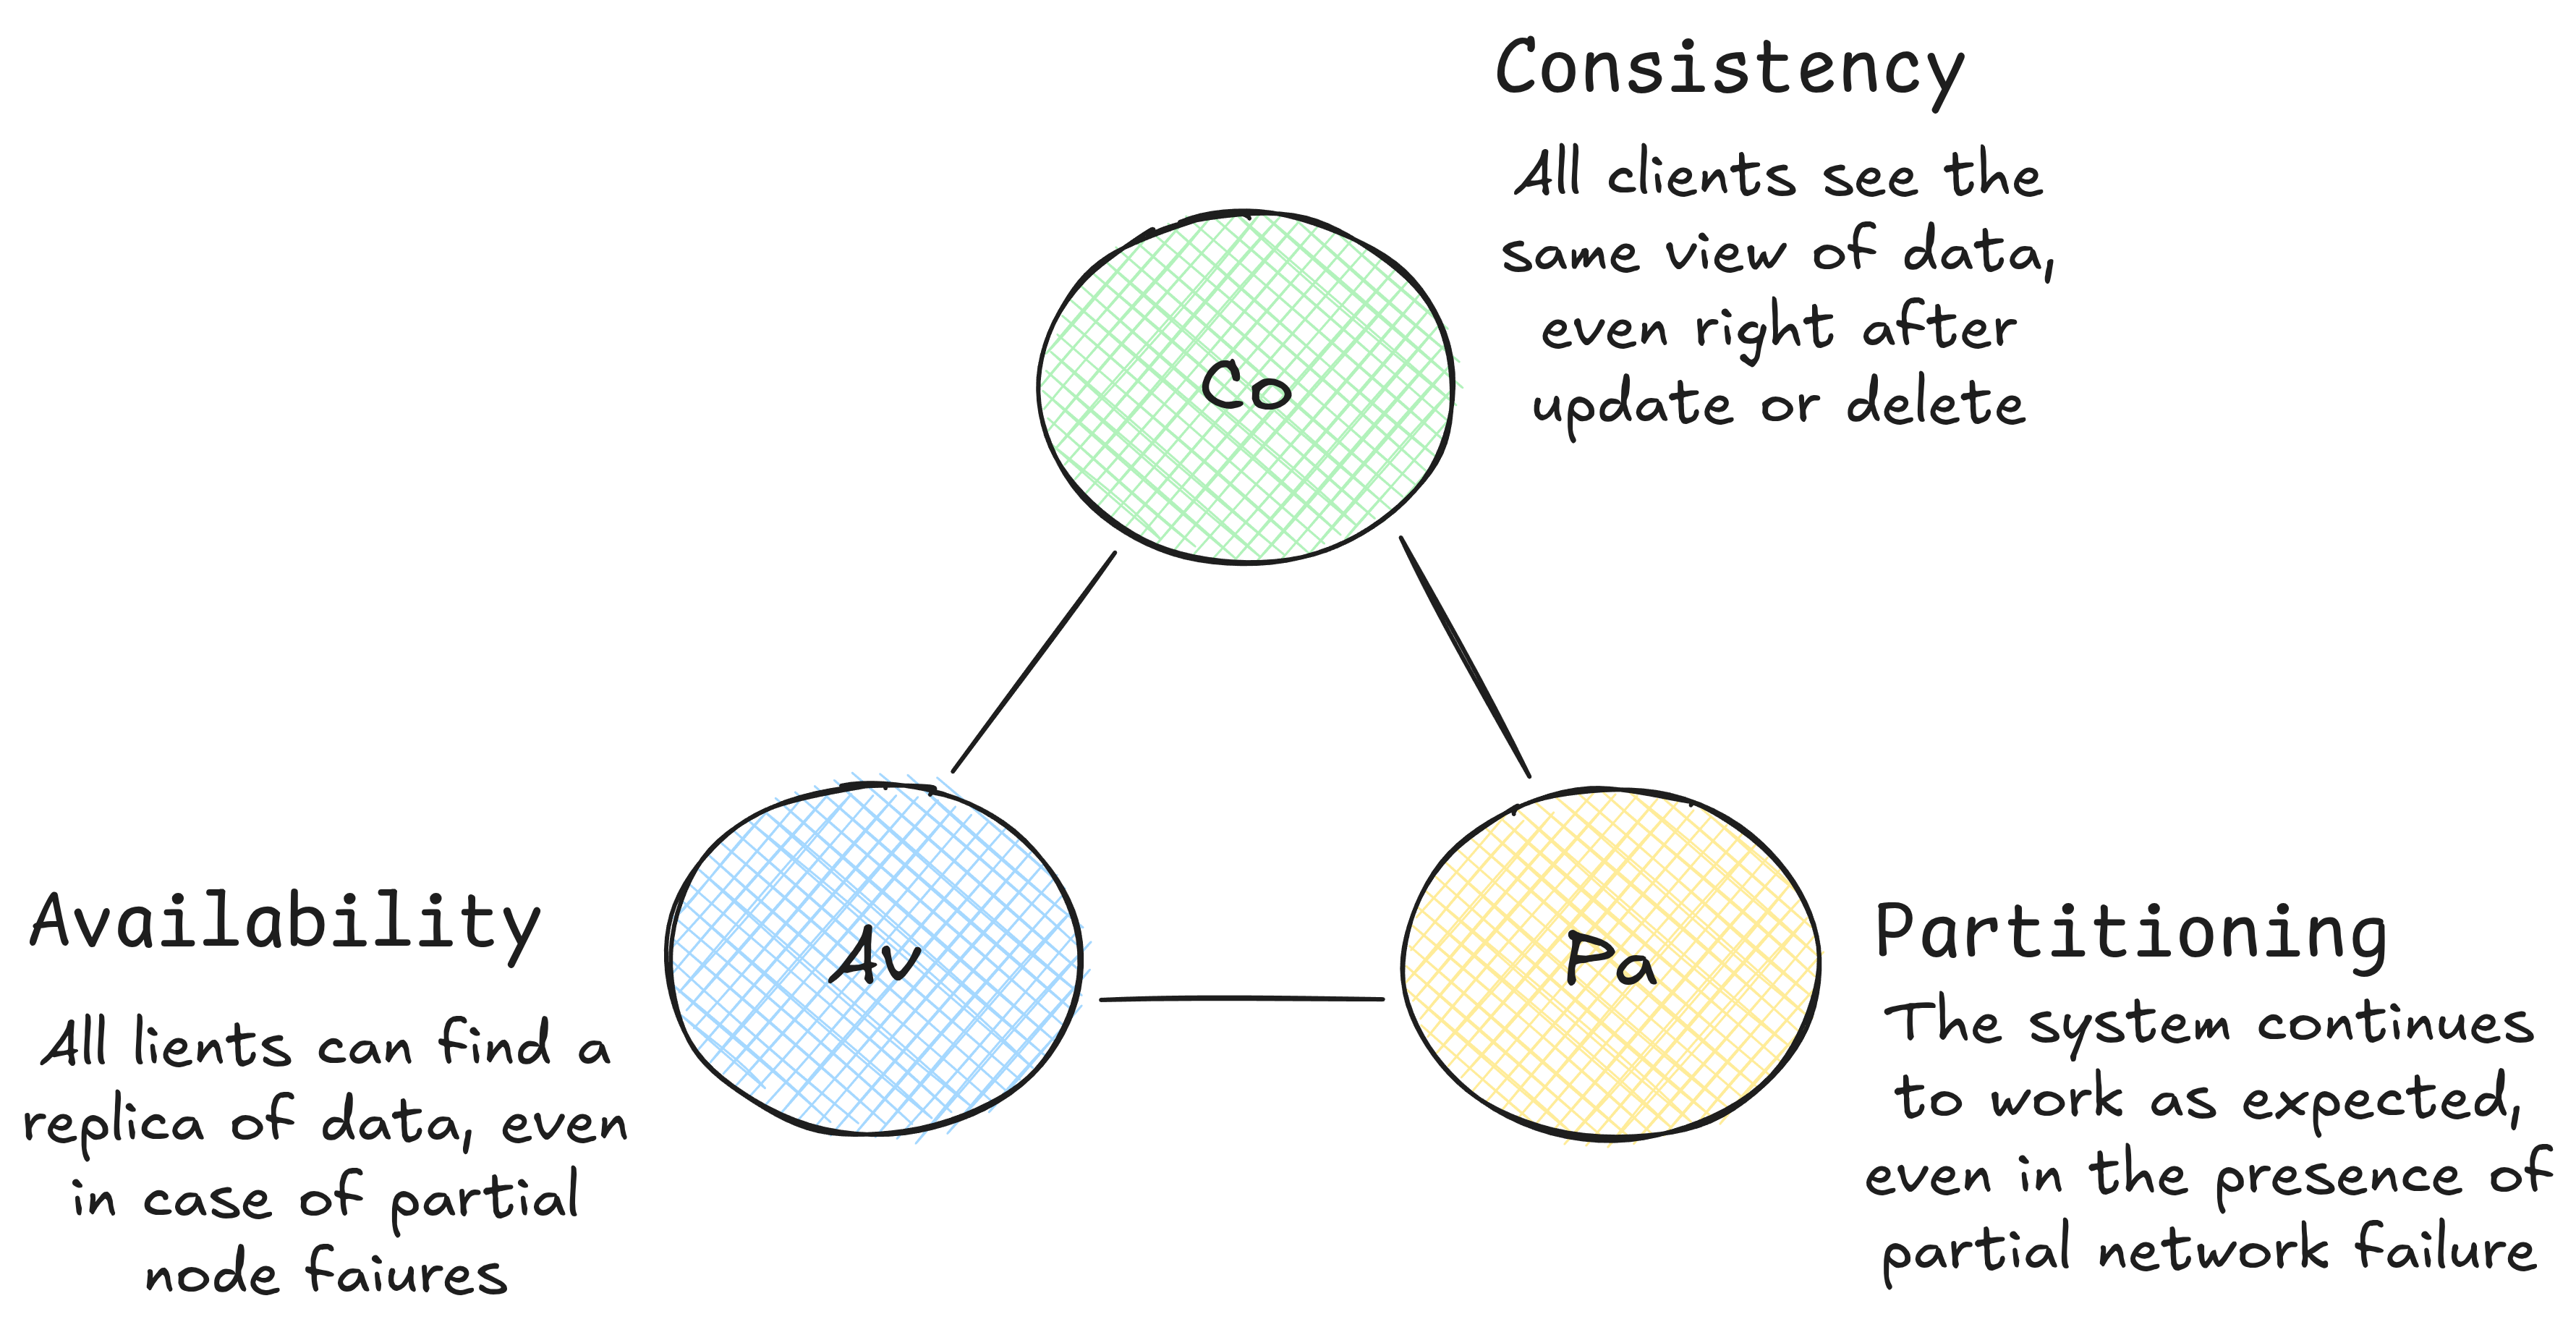
\includegraphics[width=0.9\textwidth]{images/cap.png}
    \caption[CAP theorem visualization]{\label{fig:cap}CAP theorem visualization\cite{medhat_understanding_2021}}
\end{figure}

CAP theory only describes the situation during network partitioning, which may occur in a distributed system, but it says nothing about the state in which the system is acting as a single, unpartitioned system. In such a case, the CAP theorem is extended to the so-called PACELC theorem. The PACELC theorem extends the CAP theorem (PAC) by adding the trade-off between latency and consistency (LC) even when the system is operating normally.If the system is not partitioned, it can serve only two out of three properties: latency, consistency, and availability. The logic rules behind latency, availability, and consistency are the same as in the CAP theorem. Its logic is visualized in Figure \ref{fig:pacelc}. \cite{geeksforgeeks_pacelc_nodate}

\begin{figure}[h!t]
    \centering
    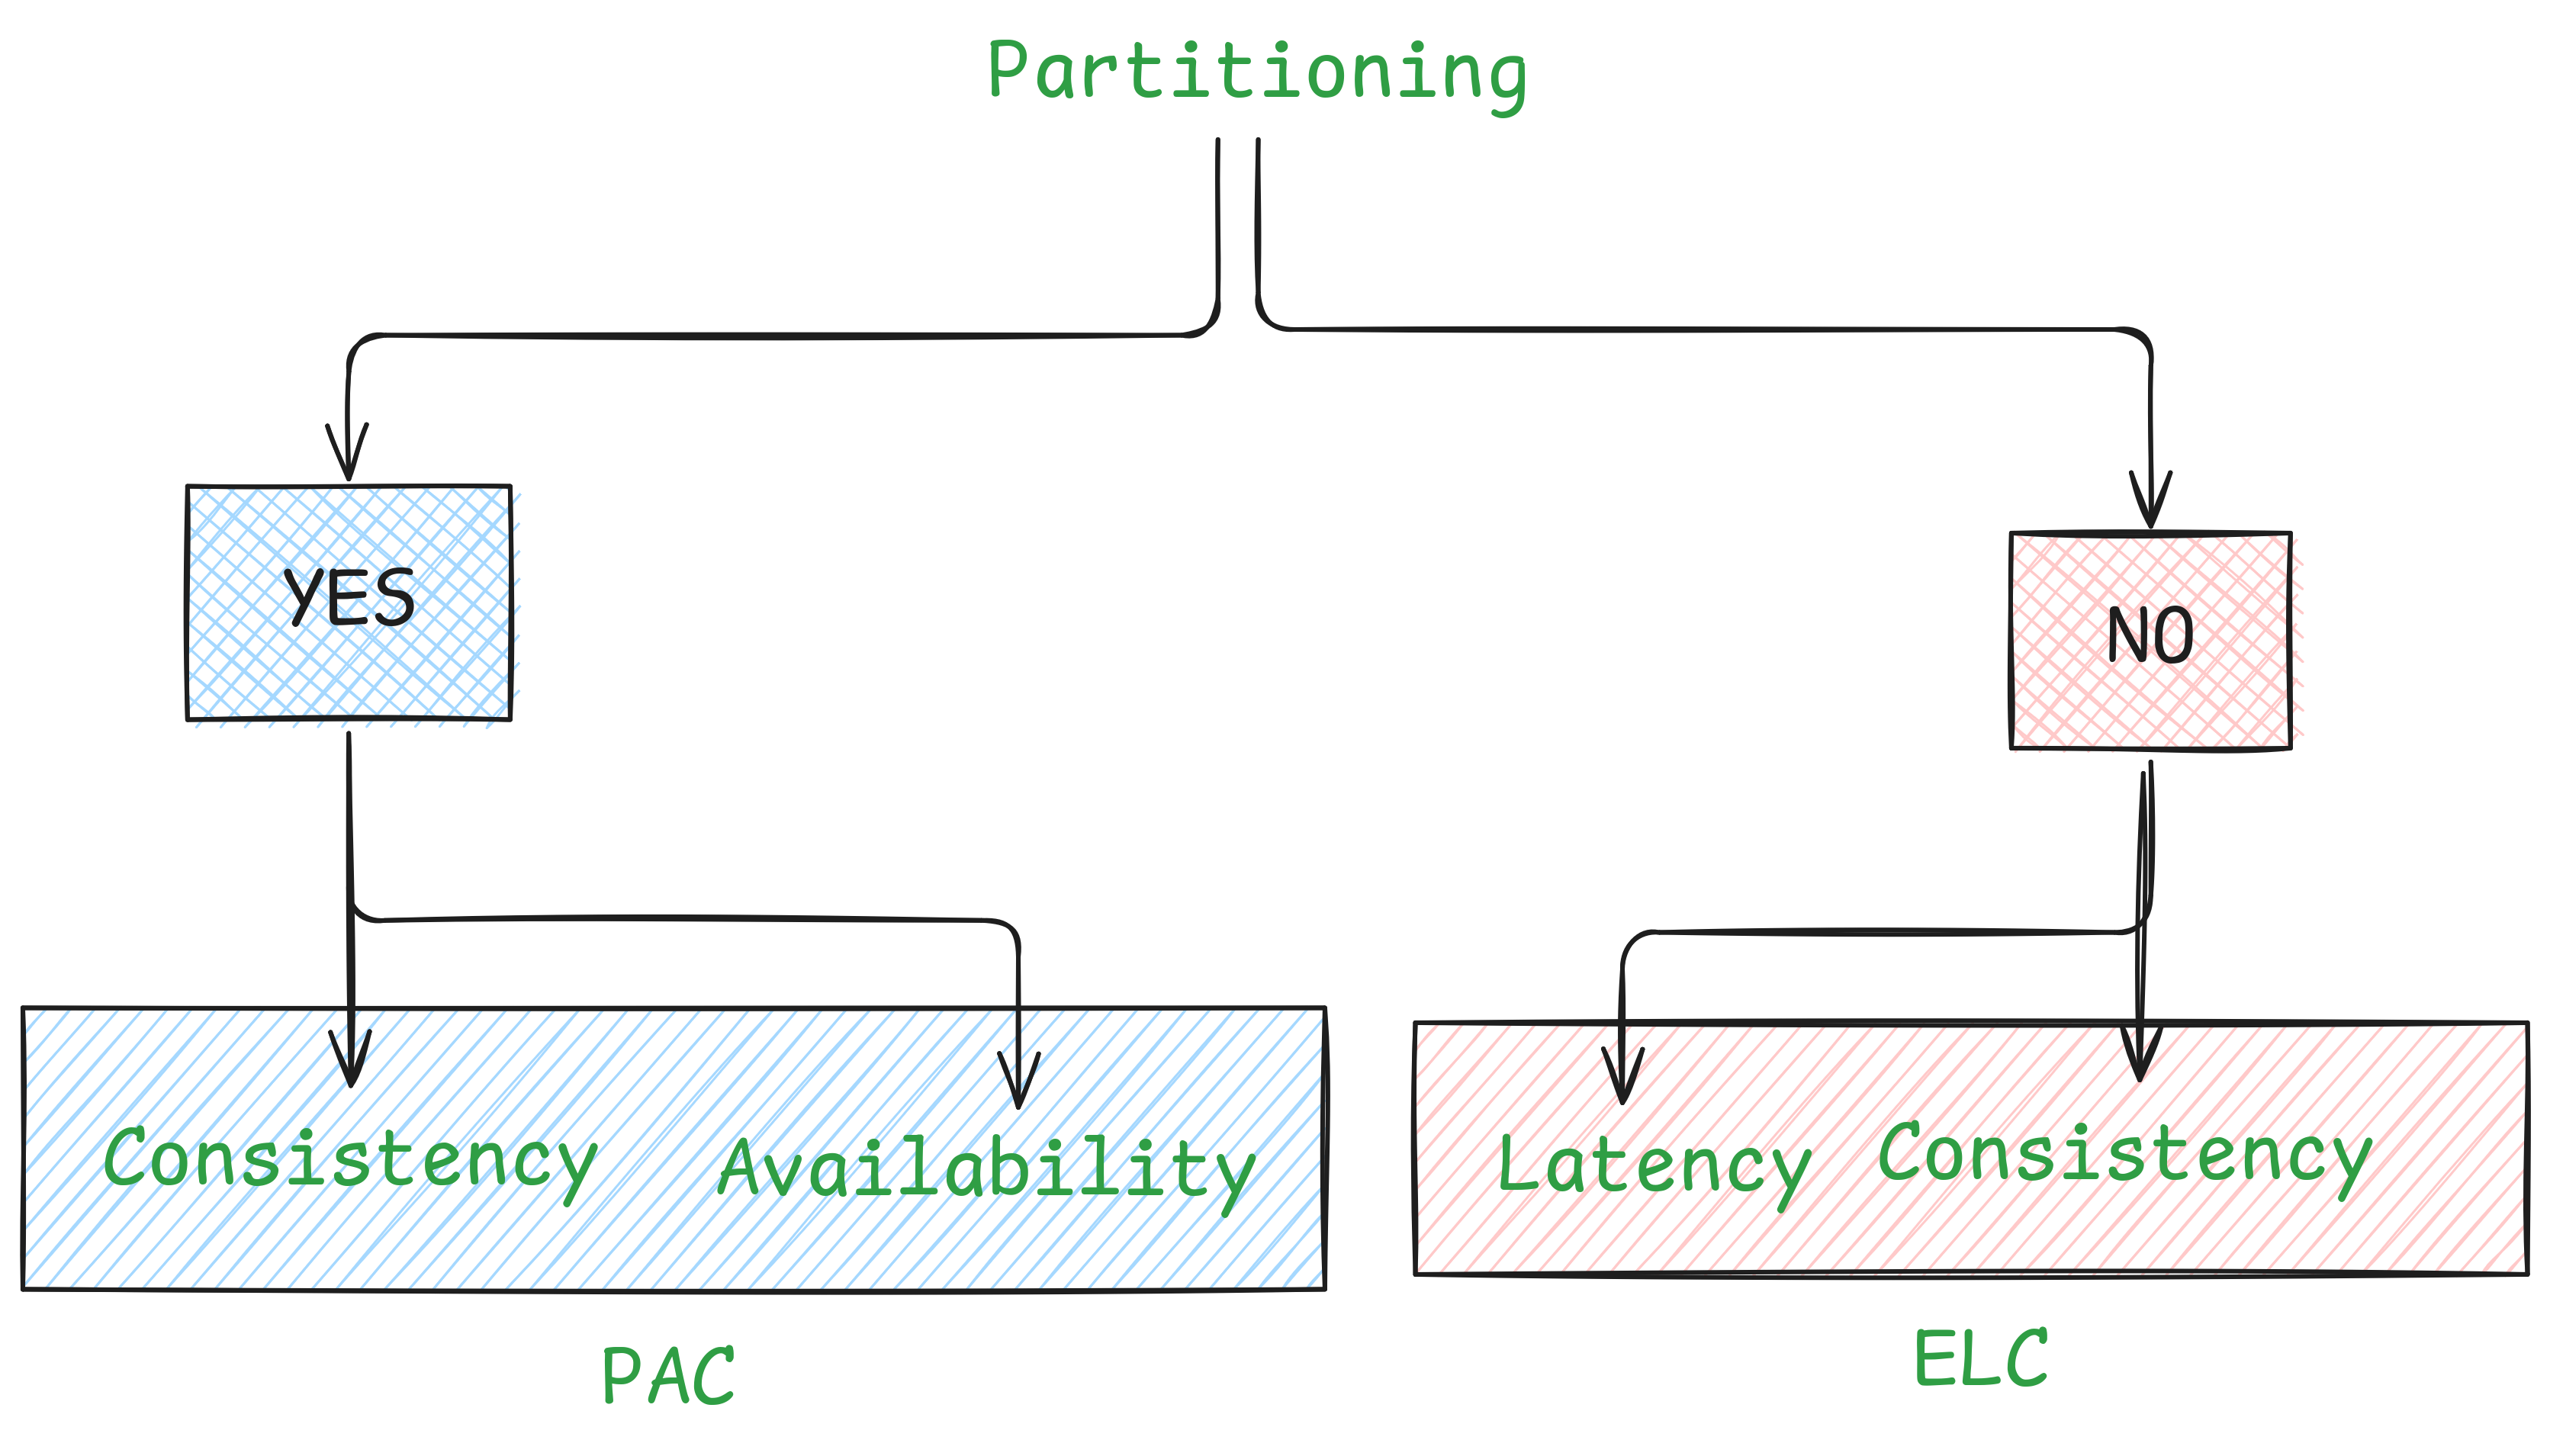
\includegraphics[width=0.9\textwidth]{images/pacelc.png}
    \caption[PACELC theorem visualization]{\label{fig:pacelc}PACELC theorem visualization (PAC, ELC)\cite{geeksforgeeks_pacelc_nodate}}
\end{figure}

\vspace{1.5em}

\subsection{Implementations of Distributed Storages}\label{sec:dfs_implementations}
\subsubsection{Ceph}\label{sec:ceph}
One of the most widely adopted scale-out storage systems is Ceph. It was originally created as a dissertation project by Sage Weil at the University of California, Santa Cruz. Today, the project is maintained by major corporations, most notably Red Hat \cite{vondra_storage_2022}. Ceph is commonly deployed as software-defined storage, approximately 75\%\cite{openstack_team_openstack_2025} of OpenStack installations (as of 2024) uses Ceph as its storage solution. It is also common choice for storage solution for Kubernetes environments. It provides a unified platform for all three primary storage abstractions: file system, object storage, and block storage. These interfaces are accessible via various APIs and protocols, including S3, iSCSI, NFS, and CSI.

The architecture of Ceph is built upon the RADOS system and the CRUSH algorithm. RADOS (Reliable Autonomic Distributed Object Store) provides an object store. The entire Ceph system operates on top of RADOS, where data are striped across RADOS objects \cite{cubefs_authors_cubefs_nodate}.

The fundamental atomic unit within RADOS is the object -- identified by a unique ID. These objects are isolated from each other and can vary in size. The object store organizes these objects into pools -- logical collections that define specific storage policies, such as the replication factor or geolocation constraints. 

The data plane of Ceph (and RADOS) is the OSD (Object Storage Daemon). An OSD is a daemon process running on a storage node, responsible for storing data on the underlying media. The OSDs form the storage cluster, which can span any number of nodes. This abstraction allows Ceph to decouple data storage from physical hardware. Administrative operations, such as managing pools and objects, are handled via the RADOS interfaces, which act as part of the control plane \cite{ceph_authors_cephio_2009}.

RADOS is a component responsible for replication, consistency, and self-healing. It communicates directly with OSD daemons to perform required operations. It is important to note that it does not implement logic for data placement. Data placement is determined by a deterministic algorithm called CRUSH.

CRUSH (Controlled Replication Under Scalable Hashing) is a deterministic algorithm that enables Ceph to efficiently manage data placement within a distributed cluster. Unlike traditional systems, CRUSH eliminates the need for a centralized metadata lookup table to locate data. Instead, clients and OSDs can independently and deterministically compute the exact location of an object based on its ID and the cluster map. This calculation relies on the CRUSH map, which defines the cluster's topology, including its hierarchical structure (e.g., racks, hosts, failure domains). By providing an object ID and the CRUSH map to the algorithm, it can deterministically compute the location of the data \cite{vondra_storage_2022, gaurav_importance_2019}.

The combination of CRUSH, the RADOS interface and the underlying object forms Ceph storage. The Ceph solution is robust and horizontally scalable. While Ceph includes additional components such as metrics servers and metadata managers (MDS) for the file system, RADOS and CRUSH are considered as the core of the architecture. Since CRUSH is just deterministic algorithm there is no need for centralize component, which could limit scalability of the system. Ceph is known to be linearly scalable if infrastructure requirements (network\ldots) are met.

To map the architecture to SDStorage, OSD daemons can be viewed as the data plane, and the CRUSH algorithm as control plane by defining data placement. Ceph supports standard fault tolerance strategies, including both replication and erasure coding.

Ceph uses (by default) a strong consistency model, which is recommended in most use cases. It can be tuned to allow eventual consistency, but such use cases are rare and not recommended. \cite{ceph_authors_welcome_2016}

\vspace{1.5em}
Overall, Ceph is meant to serve as a comprehensive, general-purpose storage platform. By unifying block, object, and file storage within a single cluster, it eliminates the need to manage distinct storages for different applications. While it demands higher hardware resources and administrative expertise compared to lightweight alternatives (like Linstore or Longhorn), its proven reliability, strict consistency model, and linear scalability make it the industry standard.
\subsubsection{LinStore}\label{sec:linstore}
Linstore is a distributed storage solution that offers only block storage capabilities. It is maintained by the same company as DRBD (Linbit) and is often referred to as an orchestrator for DRBD. It is also commonly used as a data layer for Kubernetes clusters as a Ceph solution.

Linstore provide a layer on top of DRBD that manages where data is stored across a pool of nodes. It consists of two main components: the satellite service, which represents the data plane, and the controller, which serves as the control plane.

Satellites are services running on each node and operate the node's available storage. Linstore supports two types of underlying storage. The two supported technologies are LVM and ZFS. Satellites interact with those technologies to allocate data in the pool and store data there. Data stored on nodes are replicated using DRBD.

Controller services are (often highly available) replicated services that provide an API to users, orchestrate storage, and communicate with satellites to interact with storage resources. For each requested block, the controller selects the master node in the pool where the data will be stored. Due to replication, the requested block size is limited by the maximum storage capacity of a node in the pool. For most applications, it is typically not a problem.

DRBD replication enables LinStore to load-balance reads across replicas. This makes it suitable for concurrent reads. It also makes the system fault-tolerant, since data can be restored from the underlying physical storage even when not all control-plane components are running.

Supported interfaces are object API, NVMe-oF, and iSCSI. \cite{linbit_linstor_2026}

\vspace{1.5em} %TODO
Overall, Linstore is considered a robust enterprise solution for creating distributed data pool solutions. 

\subsubsection{Longhorn}
Longhorn is another software-defined storage that offers a storage pool solution. It's meant to be used only in the Kubernetes environment by offering only interfaces compatible with Kubernetes clusters. It has a similar architecture to Linstore. It operates entirely in userspace, so it does not depend on kernel versions \cite{anderson_kubernetes_2025}. It is much simpler than previous solutions and is relatively easy to maintain and deploy, making it popular in small kubernetes deployments. Longhorn has several limitations, such as the maximum number of replicas, high CPU usage, and others\cite{simplyblock_what_2024}. Because of those limitations, it is suitable only for mid-size not-critical storage solutions \cite{longhorn_authors_longhorn_2026-1}.

\vspace{1.5em} %TODO
For quick storage, home labs in kubernetes is a good choice. It is often used in development stages, but with production QoS is usually not sufficient solution.

\subsubsection{Swift}
Swift is an eventually consistent, highly available, distributed object store primarily used in OpenStack environments. It was designed to handle large-scale, unstructured data while ensuring durability and availability in a distributed cluster. Swift’s architecture is built on a proxy-based design, where API requests are processed by proxy servers that determine the data location and route requests accordingly.

The location of the data is determined by ring computations, which serve as the core mapping mechanism between the objects' logical identifiers and their physical storage locations. This mapping is called a ring since it is based on modular arithmetic. Rings provide a control plane in Swift. This mapping is computed from multiple data structures that define placement policies for accounts, containers, and objects separately. It can distribute data based on policies, failure domains, and other parameters \cite{flament_openstack_2014}. Ring policies are mapped to structures called containers.

A container is an abstraction that groups objects with the same properties (policies). Containers are managed by container servers, which are responsible for listing objects in their respective containers. Those lists are stored and replicated between instances in SQLite DB. Metadata about objects is stored directly on the underlying FS using Extended attributes (xattrs).

Swift can work with an existing file system or use raw block devices for storage. 

Swift storage supports its own Swift REST API and the well-known S3 API. \cite{team_swift_2024}

\vspace{1.5em} %TODO
Although Swift can serve as fault-tolerant, horizontally scalable, and highly available storage, it is not as robust as the other solutions mentioned. It can be used as a sufficient object storage solution. \cite{team_swift_2024}
\subsubsection{CubeFS}\label{sec:cubefs} %TODO
CubeFS is a relatively new distributed storage system designed for high-performance data management, supporting object storage, file systems, and block storage. Currently, the project is in the incubating stage of CNCF and has become the popular solution for new infrastructures. It provides a scalable and resilient architecture by sharding data and metadata across multiple nodes while maintaining high availability and consistency through Raft-based replication mechanisms. CubeFS is commonly used in Kubernetes environments but can also be deployed outside of containerized infrastructures.

As a control plane, CubeFS uses Master nodes which are responsible for managing data and metadata shards (creating, deleting, updating, and checking consistency). The master node service can be deployed in a highly available setup with raft leader election. Its state is persisted in RocksDB, which is replicated.

Another core component is the metadata subsystem, distributed across multiple Metadata Nodes. Metadata nodes share and replicate data using the Multi-Raft replication protocol. Each metadata node maintains two B-Tree structures for storing inodes, which are kept in memory for high-speed access. For disaster recovery of metadata nodes, CubeFS also logs metadata changes to disk and periodically takes snapshots, ensuring data can be restored even in case of failure.

For data storage, Data Nodes handle actual file contents and support Erasure Coding to optimize storage efficiency and fault tolerance. CubeFS also introduces NormalExtent, a mechanism for handling large files ($\geq$ 4TiB), which allows efficient storage and retrieval of massive datasets. \cite{cubefs_authors_cubefs_nodate}

This solution can provide S3, HDFS, and POSIX API for accessing data via its Object Gateway subsystem. This should enable easy integration into various environments.

Combining sharded metadata management, Erasure Coding, and Multi-Raft replication makes CubeFS a highly scalable and reliable solution for distributed storage needs. Although CubeFS is still a new, evolving technology, it can now serve as a distributed software-defined storage solution.  \cite{cubefs_authors_cubefs_nodate}


\subsubsection{SeaweedFS (Haystack Implementation)}\label{sec:seaweedfs_haystack}
SeaweedFS is a distributed blob storage optimized for a large number of blobs. It is a project inspired by Facebook Haystack storage. Haystack is Facebook's own image storage system. Facebook declares that it stores hundreds of billions of images, which translates to tens of petabytes of data. For such a large amount of data, Facebook implemented its own solution to address its business needs and overcome limitations with the previously used NFS solution. \cite{seaweedfs_seaweedfs_2024, beaver_finding_2010}

Haystack is not publicly available as an open-source project, but its implementation designs are introduced in detail in a paper called \textit{Finding a needle in Haystack: Facebook’s photo storage}. The main idea behind Haystack is to optimize the following criteria:
Metadata overhead, High throughput and low latency, Fault tolerance, Cost effectiveness, and Simplicity. \cite{beaver_finding_2010}

The main issue with many small files is metadata management. It is necessary to limit metadata as much as possible to increase storage capacity and reduce expensive disk I/O operations for metadata lookups. Facebook states that its services require high throughput and as low latency as possible, another reason to limit metadata. To optimize latency and metadata overhead, Haystack was designed to hold all necessary metadata in main memory and use persistent storage for raw blobs (images). By such design (and other constraints -- introduced later), it is possible to serve requests (read, write) in $\Theta(1)$ disk seek access. \cite{seaweedfs_seaweedfs_2024, beaver_finding_2010}

In storage systems dealing with small file problems, it is often said that \textit{It is not a small file problem; it is a lot of files problem.}\cite{white_hadoop_2015}, to solve such a problem in Haystack, Facebook decided to group many small files/blobs into large chunks of data (typically bigger tens of GiB) -- into files also called volumes. This is possible because images are typically written once, often deleted, and then modified early. In fact, to allow Haystack and SeaweedFS architectures to work, it is necessary to not support modifications (such operations can be performed with a single delete and a single create). Volumes are large files on the server's local filesystem where the Haystack appends newly stored images. Those images (small files) are referred to as needles. They are organized in volumes, where each new needle is appended to the end of the volume till it is full (reaches maximum size). Needles consist of needed metadata and data itself -- as can be seen in Figure \ref{fig:s-volume} \cite{beaver_finding_2010}
 
\begin{figure}[h!t]
    \centering
    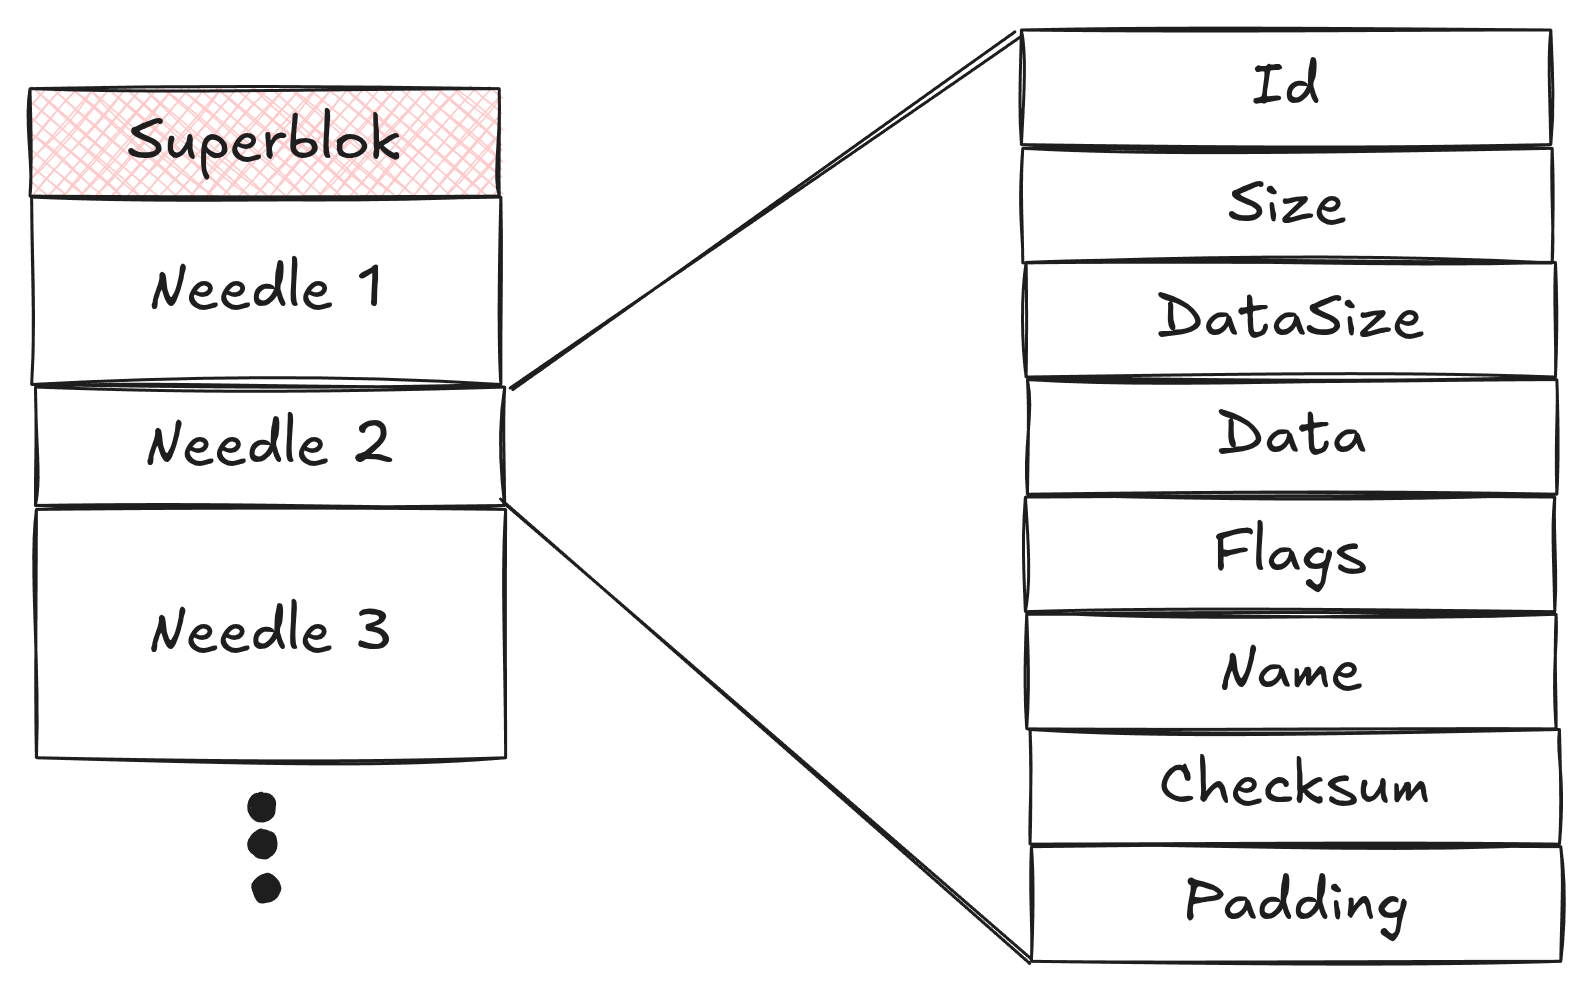
\includegraphics[width=0.6\textwidth]{images/seaweed-volume.png}
    \caption[SeaweedFS needle structure]{
      \label{fig:s-volume}
      SeaweedFS needle structure \\
      \cite{seaweedfs_authors_seaweedfsseaweedfs_2026}
      (\texttt{weed/storage/needle/needle.go)}
    }
\end{figure}

Such a volume-based architecture effectively transforms the problem of many small files into a few large ones. There are typically multiple of volumes on one system (node). \cite{beaver_finding_2010}

The organization of needles, reading, writing, and other operations are performed by a daemon running on the system. Such a system keeps opened file descriptors for each volume on the server and operates them as required. To effectively maintain volumes and needles on them, the service holds the so-called indexes. An index is a list of needles for each volume, each containing the offset and size of that needle, so they can be effectively addressed within volumes. Structure and architecture of the index can be seen in Figure \ref{fig:s-index}. When accessing the needle, the service presents an ID for the needle that encodes the needle's volume and ID.

\begin{figure}[h!t]
    \centering
    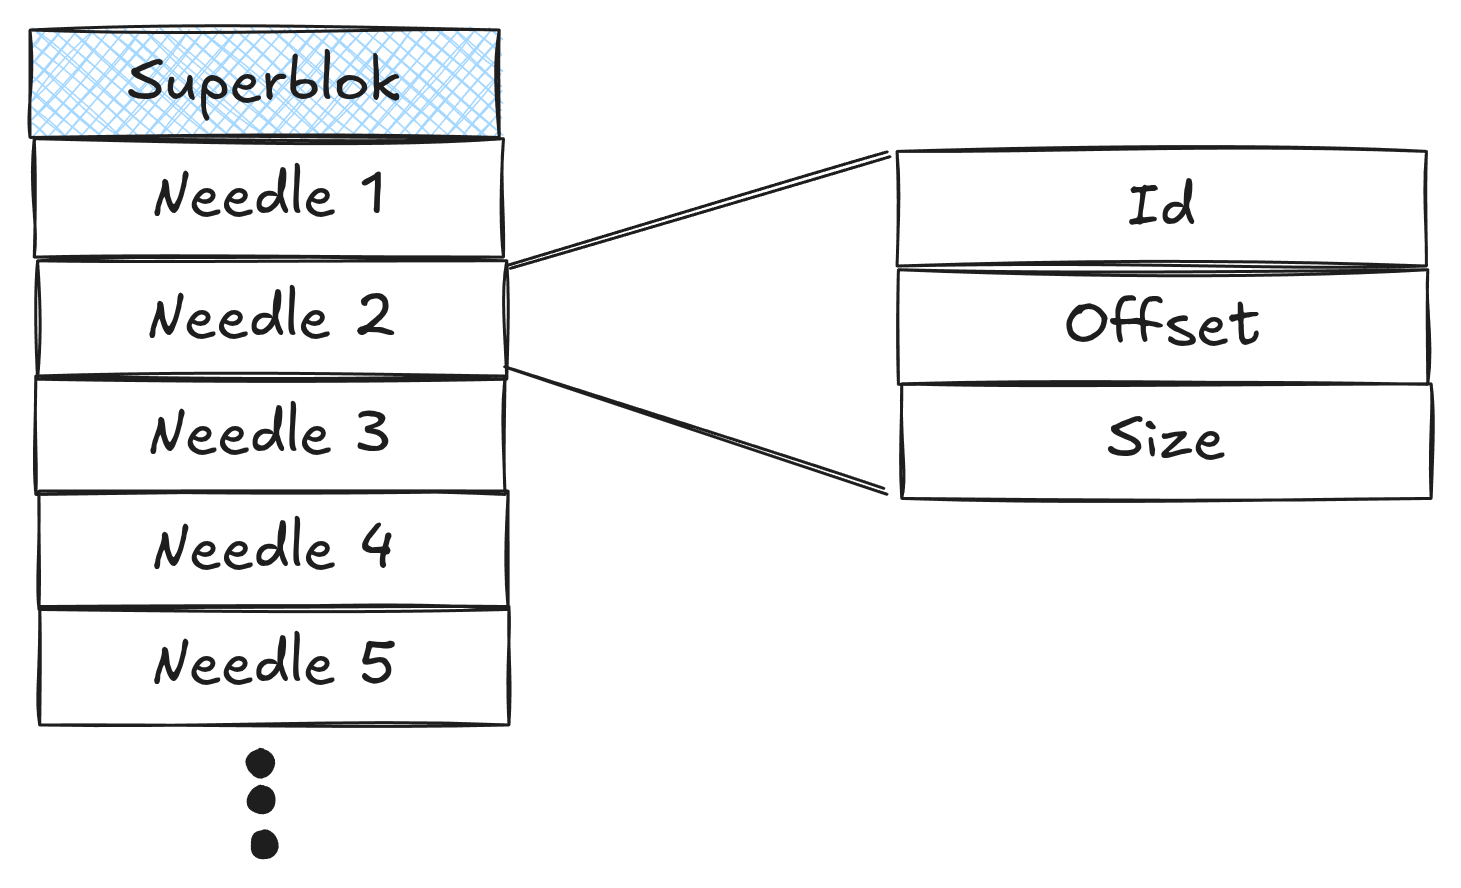
\includegraphics[width=0.6\textwidth]{images/seaweed-index.png}
    \caption[SeaweedFS needle index structure]{
        \label{fig:s-index}
        SeaweedFS needle index structure \\
        \cite{seaweedfs_authors_seaweedfsseaweedfs_2026}
        (\texttt{weed/storage/needle\_map/needle\_value.go})
    }
\end{figure}

Since an index is a collection of small data structures (in the SeaweedFS implementation, 16B), it is possible to keep all necessary data for addressing in the process's (data plane) main memory, thereby overcoming the problem of metadata overhead. It may seem that such a solution may be resource-intensive in the case of main memory. To manage 2,000,000 images, each 50 MiB in size (100 GiB in total), only $\approx$32 MB ($2*10^6 * 16B$) of main memory is required. 

Such a design of storing images as immutable objects in append-only mode introduces limitations, one of which is the inability to update or quickly delete a needle in storage. All limitations are not problematic in the context of image storage. Discussions for such limitations can be explored in detail in the Facebook Haystack paper. \cite{beaver_finding_2010}

\vspace{1.5em}

The design for managing metadata and files (needles) above is a common solution for the Haystack and SeaweedFS systems. It provides a detailed explanation of how the data plane of such systems works. In the SeaweedFS implementation service, the volume and metadata are referred to as weed volume. Another component called a master service is introduced. Since information about the implementation of the master server in the Haystack system is limited, from now on, only the SeaweedFS implementation will be discussed.

The master server is a component that orchestrates volume servers, creates volumes and enforces specified QoS. The master server operates on volumes as atomic units, treating them as if it did not know their structure. Replication, allocation, and other QoS are handled at the whole-volume level. In a replication setup, the master elects the master volume, which is the leader and append-enabled. This volume is used for appending. Read operations may be handled by multiple replicas based on the volume pool state. Any recovery and fault tolerance is also handled at volume levels. \cite{seaweedfs_seaweedfs_2024}

SeaweedFS implementation provides full access to Kubernetes, POSIX, S3, Hadoop, and WebDAV interfaces. For data durability, mainly replication is used, but erasure coding is also supported. Concrete abilities will be discussed in practical part of this thesis. \cite{seaweedfs_seaweedfs_2024}

\vspace{1.5em}
In summary, SeaweedFS addresses the specific scalability challenges associated with storing billions of small files. By adopting the Haystack architecture's approach of reducing disk I/O to Θ(1) and managing metadata in memory, it achieves high throughput with minimal overhead. It is an ideal choice for high-volume blob stores, content delivery networks, and data lakes where raw performance and storage efficiency are prioritized over the complex feature sets of general-purpose systems like Ceph.

\chapter{Theoretical Part -- Data Processing}\label{ch:data_processing}
The goal of this thesis is to design a data processing pipeline with an appropriate storage system suitable for the described use case. This chapter will focus on the computational and data-processing part. It is assumed that the necessary storage solutions already exist, and only the theory of data processing will be discussed to build fundamental knowledge that will later be applied in the implementation.

The goal of this chapter is to introduce the fundamentals, serving as a starting point for any similar data processing system.

\section{Data Processing}
In the thesis, data processing refers to the process of moving and transforming selected binary data.

There are three distinct types of data processing systems that need to be distinguished. Each of these systems requires different solutions that are optimized and tuned to its needs.
\begin{itemize}
    \item \textbf{Online (service systems)} \\
    The online (service) data processing system is a request-based system in which data are processed per client request. Processing begins when the system receives a request, and the service must produce output to respond to the client. In such a system, the main criterion (to optimize for) is response time -- the latency between request and response, and parameter availability of the system. Those two are considered the most important in such a system.
    \item \textbf{Offline processing systems (batch systems)} \\
    The batch-processing (offline) system is typically used to process large amounts of input data at once. This type of processing is not focused on speed (since it may take from a few minutes to several days), but is optimized for throughput. Such processes are often run periodically and are scheduled as jobs. It is not focused on availability, but on quality and throughput.
    \item \textbf{Stream processing systems (near-real-time systems)} \\
    Stream processing lies between offline and online processing. Like in batch processing, it typically process a large amount of work and processes them in parallel; it also does not typically produce a response, but some output, which is later stored in any type, including a database, event, file, etc. \\
    On the other hand, it usually processes the data as soon as the event or job is available to the system. This is more similar to online processing.
\end{itemize}\cite{kleppmann_designing_2017}

This thesis focuses on stream processing systems (also known as near-real-time systems). Since stream processing combines online and offline processing, it needs to incorporate concepts from both. The method for combining both systems and building a streaming data pipeline system will be discussed in Section \ref{sec:pipeline_architectures} 

\section{Pipelines}
In modern software architecture, the mechanism responsible for moving and transforming data is called a data pipeline. It usually involves the transport of data, its validation, transformation, and management during transit. In the context of the thesis, the pipeline includes downloading images, processing them, deriving image metadata, storing data in internal storage, computing image embeddings, and outputting the embeddings. \cite{kleppmann_designing_2017}

A data pipeline is, in general, any automated process that runs a predefined sequence of operations. It begins with a clearly defined input, which can be the data itself or information on how to access the data. When data enter the pipeline, they are processed by a series of steps. Those steps can always be represented as an acyclic graph (DAG). At the end of the pipeline, it provides a clear data-processing output or stores it in the required systems. This makes the whole pipeline well-defined and clear, so it can be reproduced at any time for any amount of data. \cite{kleppmann_designing_2017}

In practical implementations, individual operations (part of the pipeline) are frequently aggregated into logical units called \textit{jobs}. They encapsulate a specific sequence of related tasks -- such as downloading, resizing, and saving.

\subsection{Job}\label{sec:job}
Units of operations in the pipeline are often referred to as jobs. Jobs are parts of a pipeline that can be logically isolated. Those parts are typically responsible for the subtasks of the pipeline, and by chaining them together, they form a whole (data) pipeline. Such parts can be understood as small programs (a list of instructions) that convert well-defined input to well-defined output (same as the whole pipeline). In a more abstract sense, jobs can be understood as smaller pipelines that together form a single larger pipeline.

The idea of jobs is an old concept in software engineering known as modularity. Modularity offers a new way to approach problems by breaking them into smaller pieces (rather than maintaining a single monolithic solution). Even though modularity is an old, intuitive concept, it has become more popular with the rise of distributed systems and microservice architectures.\cite{reis_fundamentals_2022}\footnote{As many think in modern computer science.}

Isolating a series of instructions in a pipeline into units called jobs allows more control over the input and output of each job, breaks tight coupling, and defines well-defined points throughout the pipeline. Such points can later be used for failure reporting, recovery, etc. Among other advantages, breaking pipelines into loosely coupled chunks allows better scalability and planning. \cite{reis_fundamentals_2022}

\subsection{Pipeline -- Chaining Jobs}
As defined in Section \ref{sec:job}, a job represents a single logical unit of work. However, complex data processing tasks rarely consist of a single job. Instead, they require the sequential or parallel execution of multiple distinct steps (jobs). This composition of jobs is referred to as \textit{chaining}, and the resulting structure forms the \textit{data pipeline}.

By chaining jobs, the pipeline acts as a layer that manages the flow of data from one unit to the next. This architecture offers several advantages over monolithic data processing scripts.

\subsubsection*{Fault Tolerance and Recovery}
One benefit of breaking a pipeline into units is improved recovery when execution fails. In a monolithic process, each error must be handled separately, and recovery usually requires restarting the entire process from the beginning. In a chained pipeline, errors must be handled the same way as in monolithic code, but each job can serve as a checkpoint, allowing recovery. 

If a specific job fails, the system can identify exactly which step encountered an error. Because the state of the data is defined at the input and output of every job, the pipeline can often be restored, starting only from the failed job, rather than re-starting the entire process. This \textit{unit of failure} approach significantly reduces the cost of errors and simplifies debugging.

\subsubsection*{Modularity and Replaceability}
Decomposing a complex pipeline into a chain of jobs enforces modularity. Since each job is a unit with a strictly defined input and output, individual jobs can be updated, optimized, or entirely replaced without affecting the rest of the pipeline.

For example, a specific image resizing algorithm in the middle of a pipeline could be swapped for a more efficient library. As long as the input/output interface remains consistent, the surrounding jobs (downloading or storing) remain unchanged. This decoupling enables easier maintenance and iterative system improvement.

\subsubsection*{Scalability and Distributed Execution}
Pipeline architecture is, by design, suitable for distributed computing. Because jobs are isolated, they do not necessarily need to run on the same physical machine. A pipeline orchestrator can distribute different jobs across multiple nodes in a cluster.

This enables horizontal scaling: if the image embedding job is computationally intensive and limits throughput, it can be scaled out to run across multiple worker nodes in parallel, while lighter jobs (such as metadata extraction) run on fewer resources. This flexibility allows the system to maximize resource utilization and throughput.

The dependencies between jobs naturally form a Directed Acyclic Graph (DAG). By explicitly defining which jobs depend on the output of others, the system can identify pipeline branches that are independent of one another. These independent branches can be executed in parallel across different nodes, significantly reducing the total processing time. \cite{kleppmann_designing_2017}

\section{Pipelines for Data Processing Systems}\label{sec:pipeline_architectures}
As discussed in the previous Section \ref{ch:data_processing}, data processing systems can be categorized into three distinct types: online (service) systems, offline (batch) systems, and stream processing systems. In the introduction to this thesis, it was established that the primary goal is to design and implement a stream processing pipeline.

Since stream processing is conceptually a hybrid of online and offline processing, it inherits characteristics from both. The following section will describe online, offline, and lastly stream solutions, which will often be a combination of both approaches. The text will discuss 4 components that need to be designed for such pipelines: input, connector, worker, and output. To better understand these architectural designs, refer to Figures \ref{fig:online-pipeline}, \ref{fig:offline-pipeline}, \ref{fig:stream-pipeline} during reading.

All architectural designs come from different needs, and ways of data processing like specified above.

\subsection{Data Input and Triggering}
The first fundamental difference between the architectures is how data enter the system and what triggers the processing.

\begin{itemize}
    \item \textbf{Online:} In online systems, input is typically handled via standard network protocols such as REST (HTTP) or gRPC. The trigger is external (a request), and processing begins immediately upon receipt of a request. Requests are typically sent by the user or other systems, which use the pipeline.
    \item \textbf{Offline:} Offline systems do not respond to any external request; they rely on a scheduled or manual trigger. The input is usually a bounded set of data (work) available in some form (typically storage). The process is initiated by a human operator or a time-based scheduler (e.g., CRON) once all required data are collected and the necessary resources to run the pipeline are available.
    \item \textbf{Stream:} Stream pipelines process data that arrive in the system without knowing when it happens and at what load, typically using an event-driven input model. To handle input, the use of a queue or an event log to hold processing requests for the pipeline is required. Processing is triggered by the arrival of an event. As soon as data are pushed to the queue, the pipeline consumes it, combining the automated nature of online systems with the decoupling of offline systems. Such an architecture allows the system to react to incoming messages almost immediately (near real-time) and still handle large loads of data to be processed by keeping requests in a job queue.

\cite{kleppmann_designing_2017, reis_fundamentals_2022}
\end{itemize}

% refrazed
\subsection{Connectors and Transport}
Transporting data between different stages (jobs) of a pipeline requires different solutions for each type of data processing system. Solutions influence the capacity, latency, and durability of stage connectors (which hold the state of processed data).

\begin{itemize}
    \item \textbf{Online:} Communication is primarily handled via the network. A network enables minimizing latency, which is needed for online processing. A downside of using the network is the inability to recover from failures at any stage of the pipeline, since data are not persistent. This is typically not a problem since the user can receive an error response and a repeat request if needed. \\
    Services typically communicate synchronously over the network, expecting an immediate reaction.
    \item \textbf{Offline:} The primary connector is \textit{storage}. One stage of a job writes data to a storage or database, and the next stage reads from that storage. The storage acts as the interface between steps. This allows recovery from any stage where an error may have occurred. Introducing storage may introduce additional latency. This should not be a common issue, as offline processing typically runs for extended periods and the latency is not significant across the entire process.
    \item \textbf{Stream:} To handle continuous flow and potential pressure, stream systems typically use \textit{Message Queues} (or Message Brokers). The queue acts as a buffer, ensuring that data are not lost if processing requests spike and the pipeline is not scaled to handle such a load.

\cite{kleppmann_designing_2017}
\end{itemize}

% refrazed
\subsection{Resource Allocation}
The strategy for resource allocation and worker lifecycle differs significantly based on the expected load pattern.

\begin{itemize}
    \item \textbf{Online:} Jobs must always be running and available to serve responce with as low latency as possible. Even during idle periods, resources are reserved to ensure immediate response capability when a request arrives. Such solutions are resource-intensive because they have to keep running workers to handle the largest expected load.
    \item \textbf{Offline:} Workers are ephemeral. During idle times, zero workers are running. When a job is triggered, the system spawns as many workers as the hardware resources or parallelization logic allow, runs them at full capacity, and terminates them upon completion. Sections in pipelines are typically allocated to each job independently to achieve high throughput. This is possible because the data state between stages is stored permanently.
    \item \textbf{Stream:} Stream processing uses scalable workers. While the system requires a baseline number of running workers to ensure availability (as in online systems), it must scale dynamically during peak traffic to maintain throughput. This ensures resource efficiency -- scaling up during high load and scaling down (but not to zero) during low load.
\end{itemize}

\subsection{Output and Results}
Finally, the systems differ in what they produce as a result of the processing.

\begin{itemize}
    \item \textbf{Online:} The output is a response to the user or the system. The system must return data or a confirmation status back to the client that initiated the request.
    \item \textbf{Offline:} The output is typically a report or a transformed dataset stored in a database/storage. There is no direct client waiting for a response.
    \item \textbf{Stream:} Stream pipelines often produce both. They generate reports (aggregated data stored for analysis) and can also trigger responses or side effects (such as alerts or push notifications) in real-time.
    
\cite{kleppmann_designing_2017}
\end{itemize}

\begin{figure}[h!t]
    \centering
    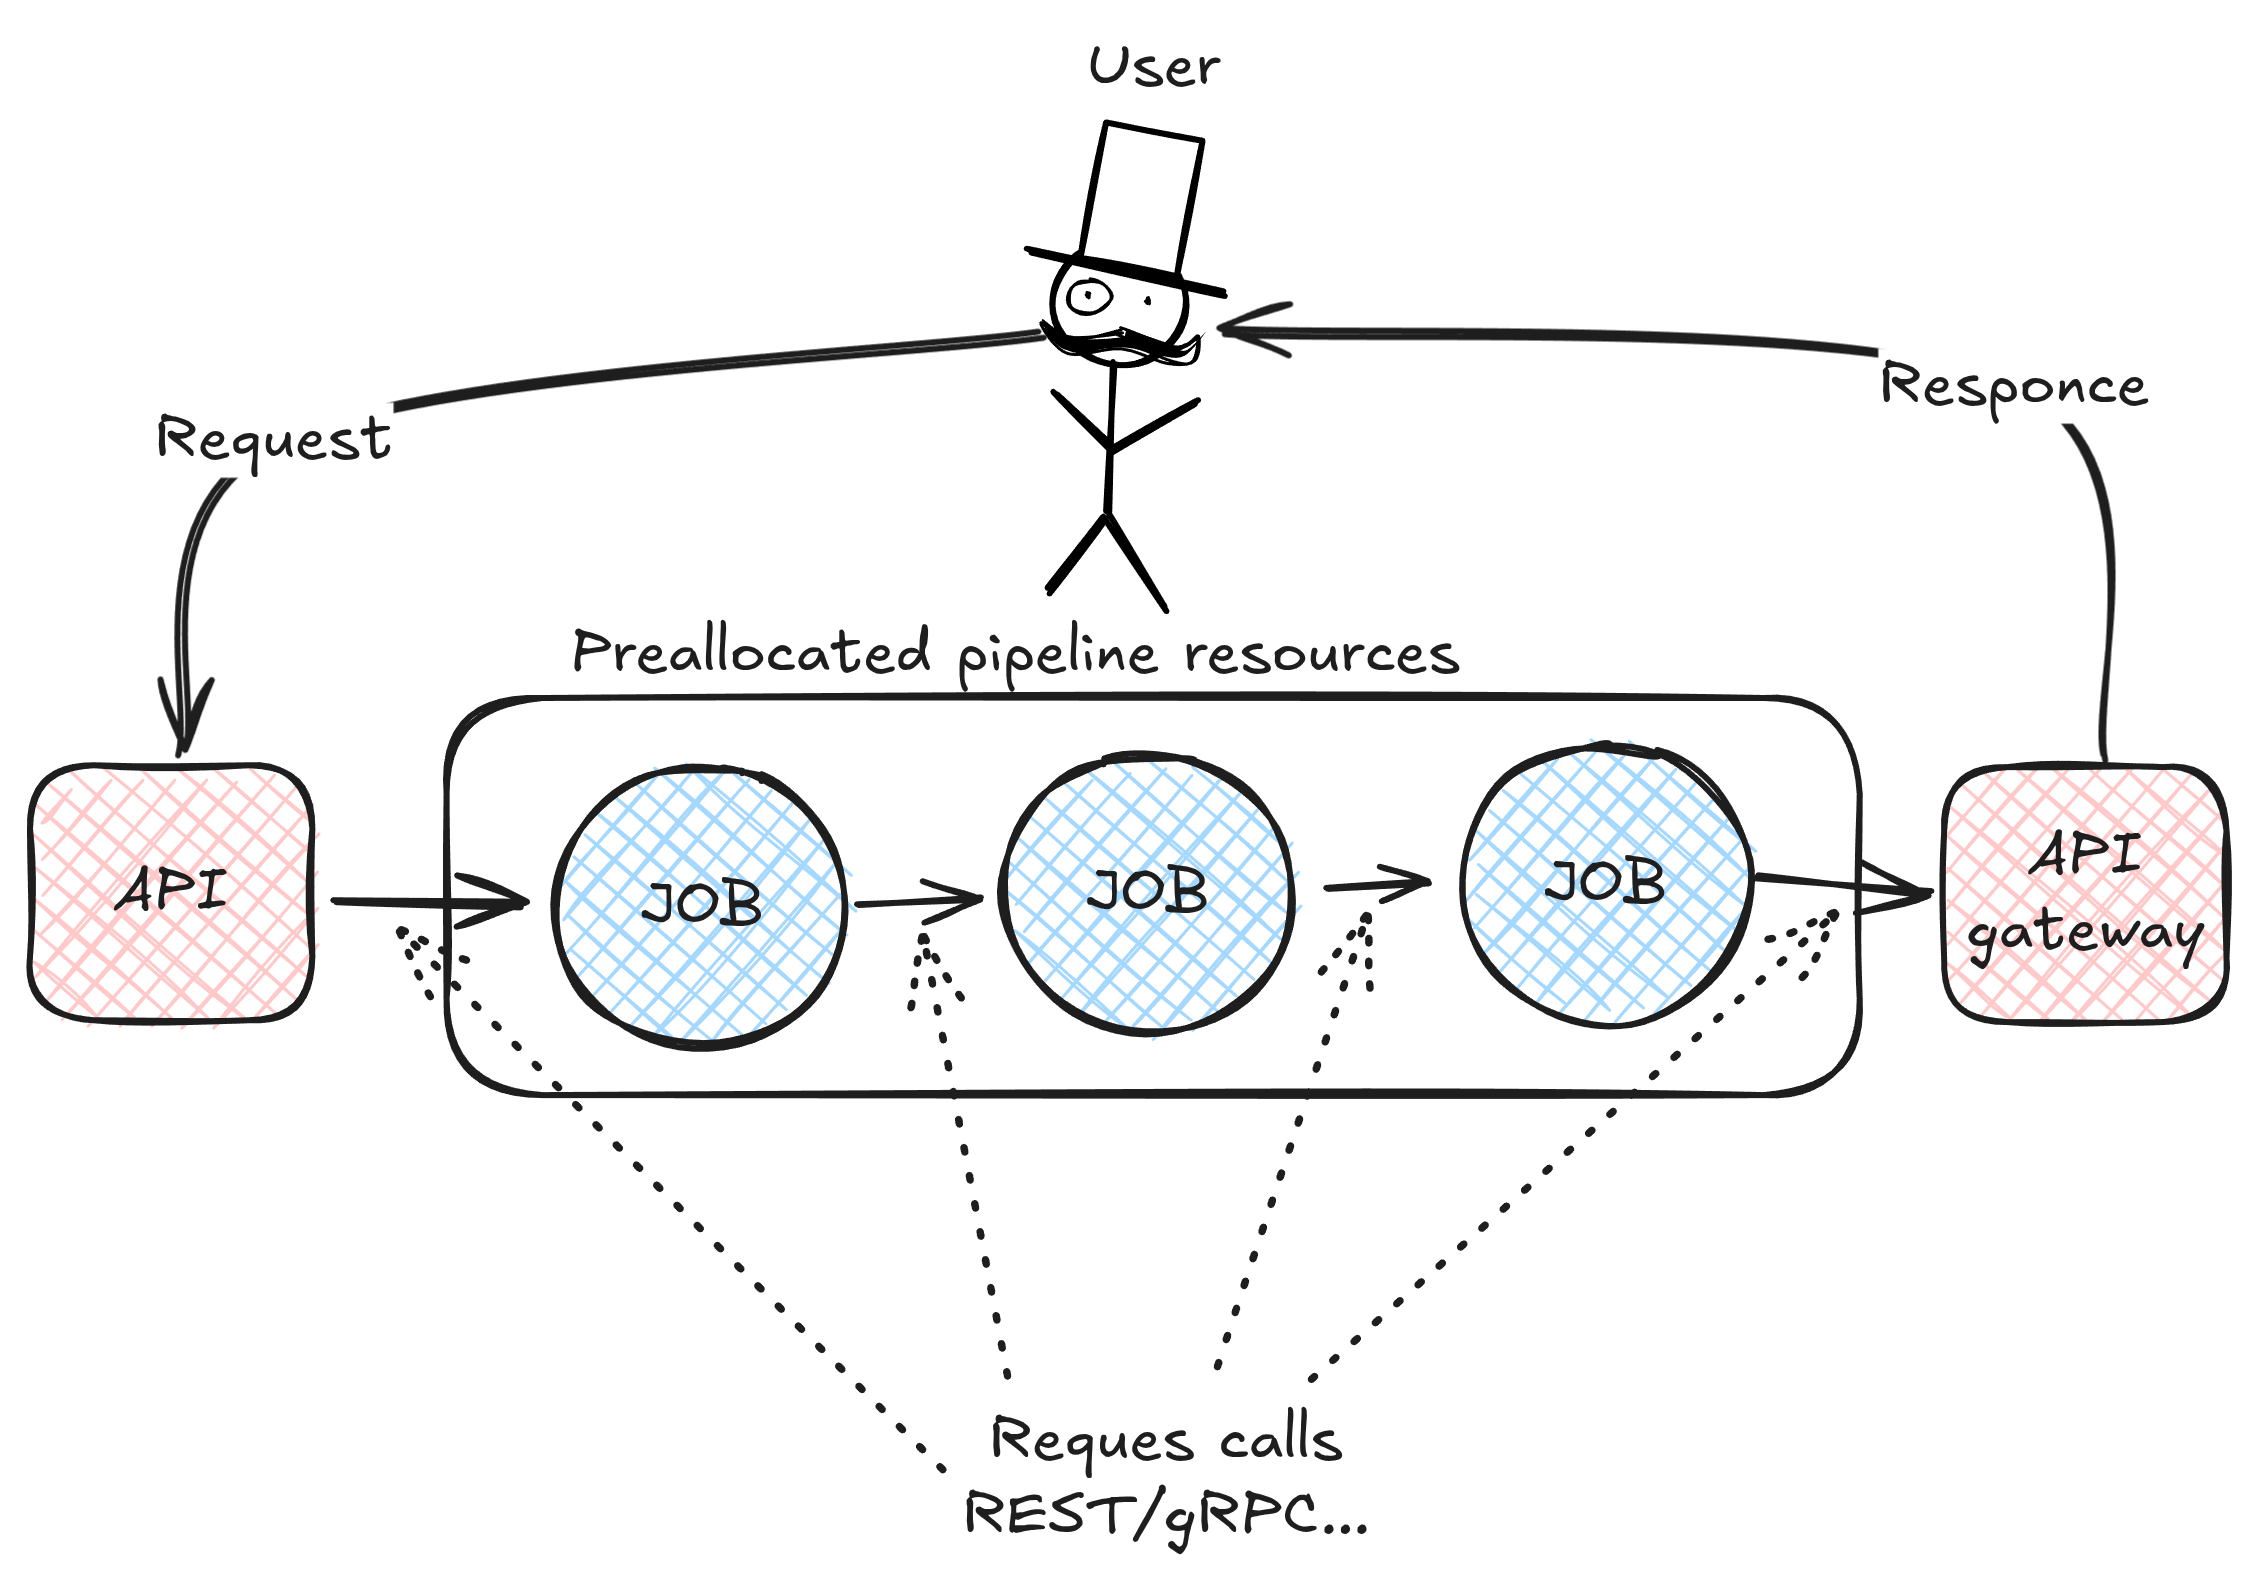
\includegraphics[width=0.8\textwidth]{images/online-pipeline.png}
    \caption{\label{fig:online-pipeline}Online pipeline}
\end{figure}

\begin{figure}[h!t]
    \centering
    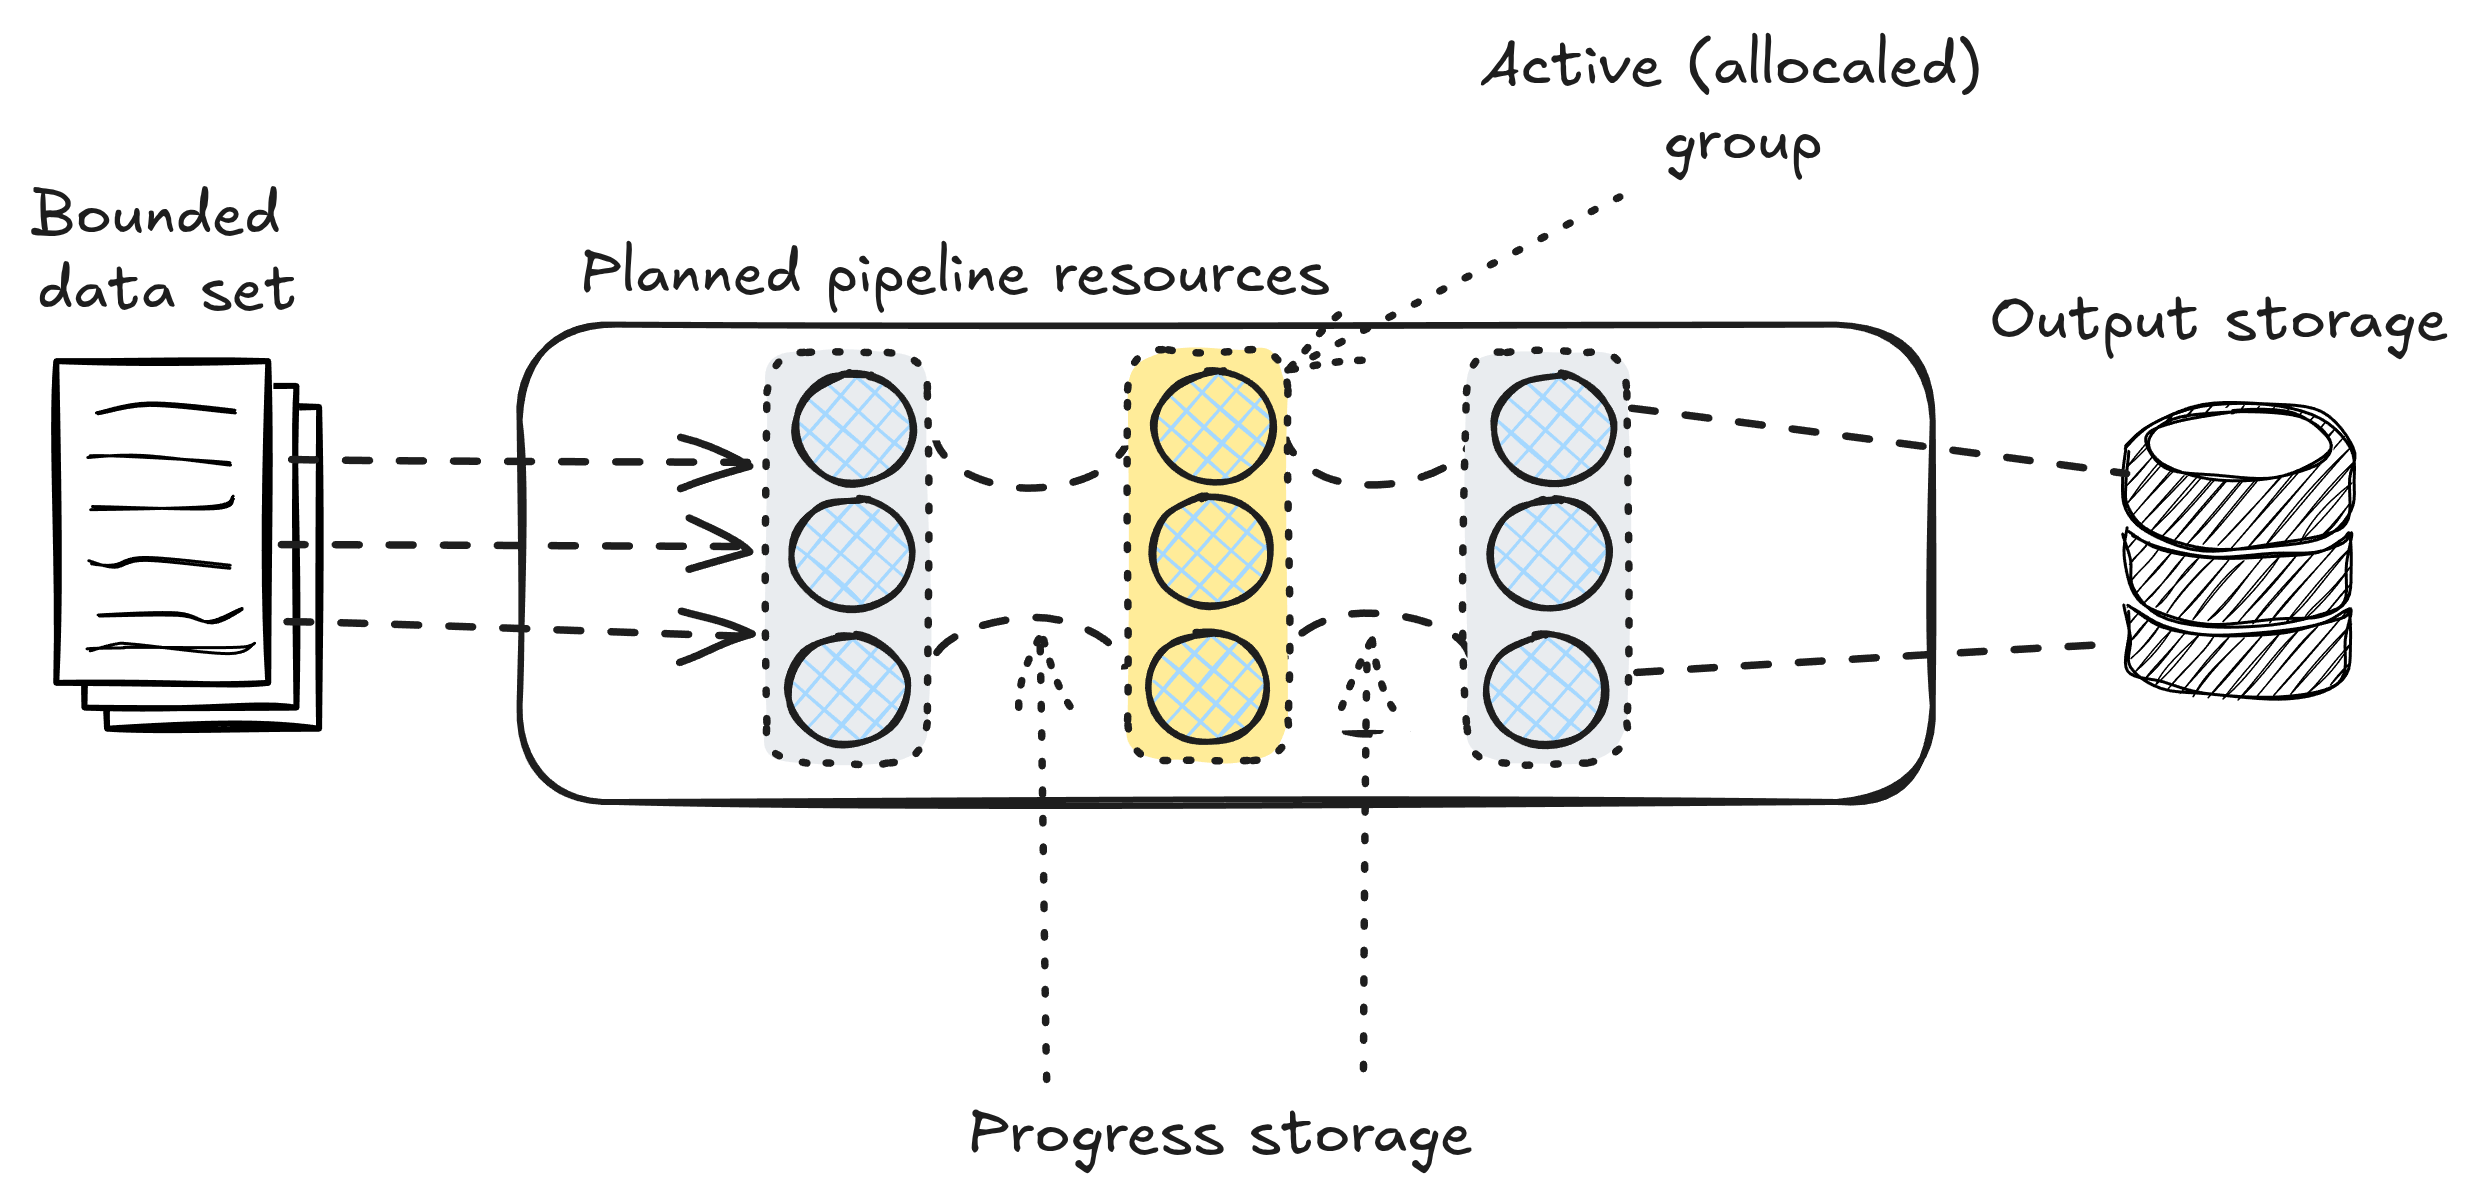
\includegraphics[width=0.8\textwidth]{images/offline-pipeline.png}
    \caption{\label{fig:offline-pipeline}Offline pipeline}
\end{figure}

\begin{figure}[h!t]
    \centering
    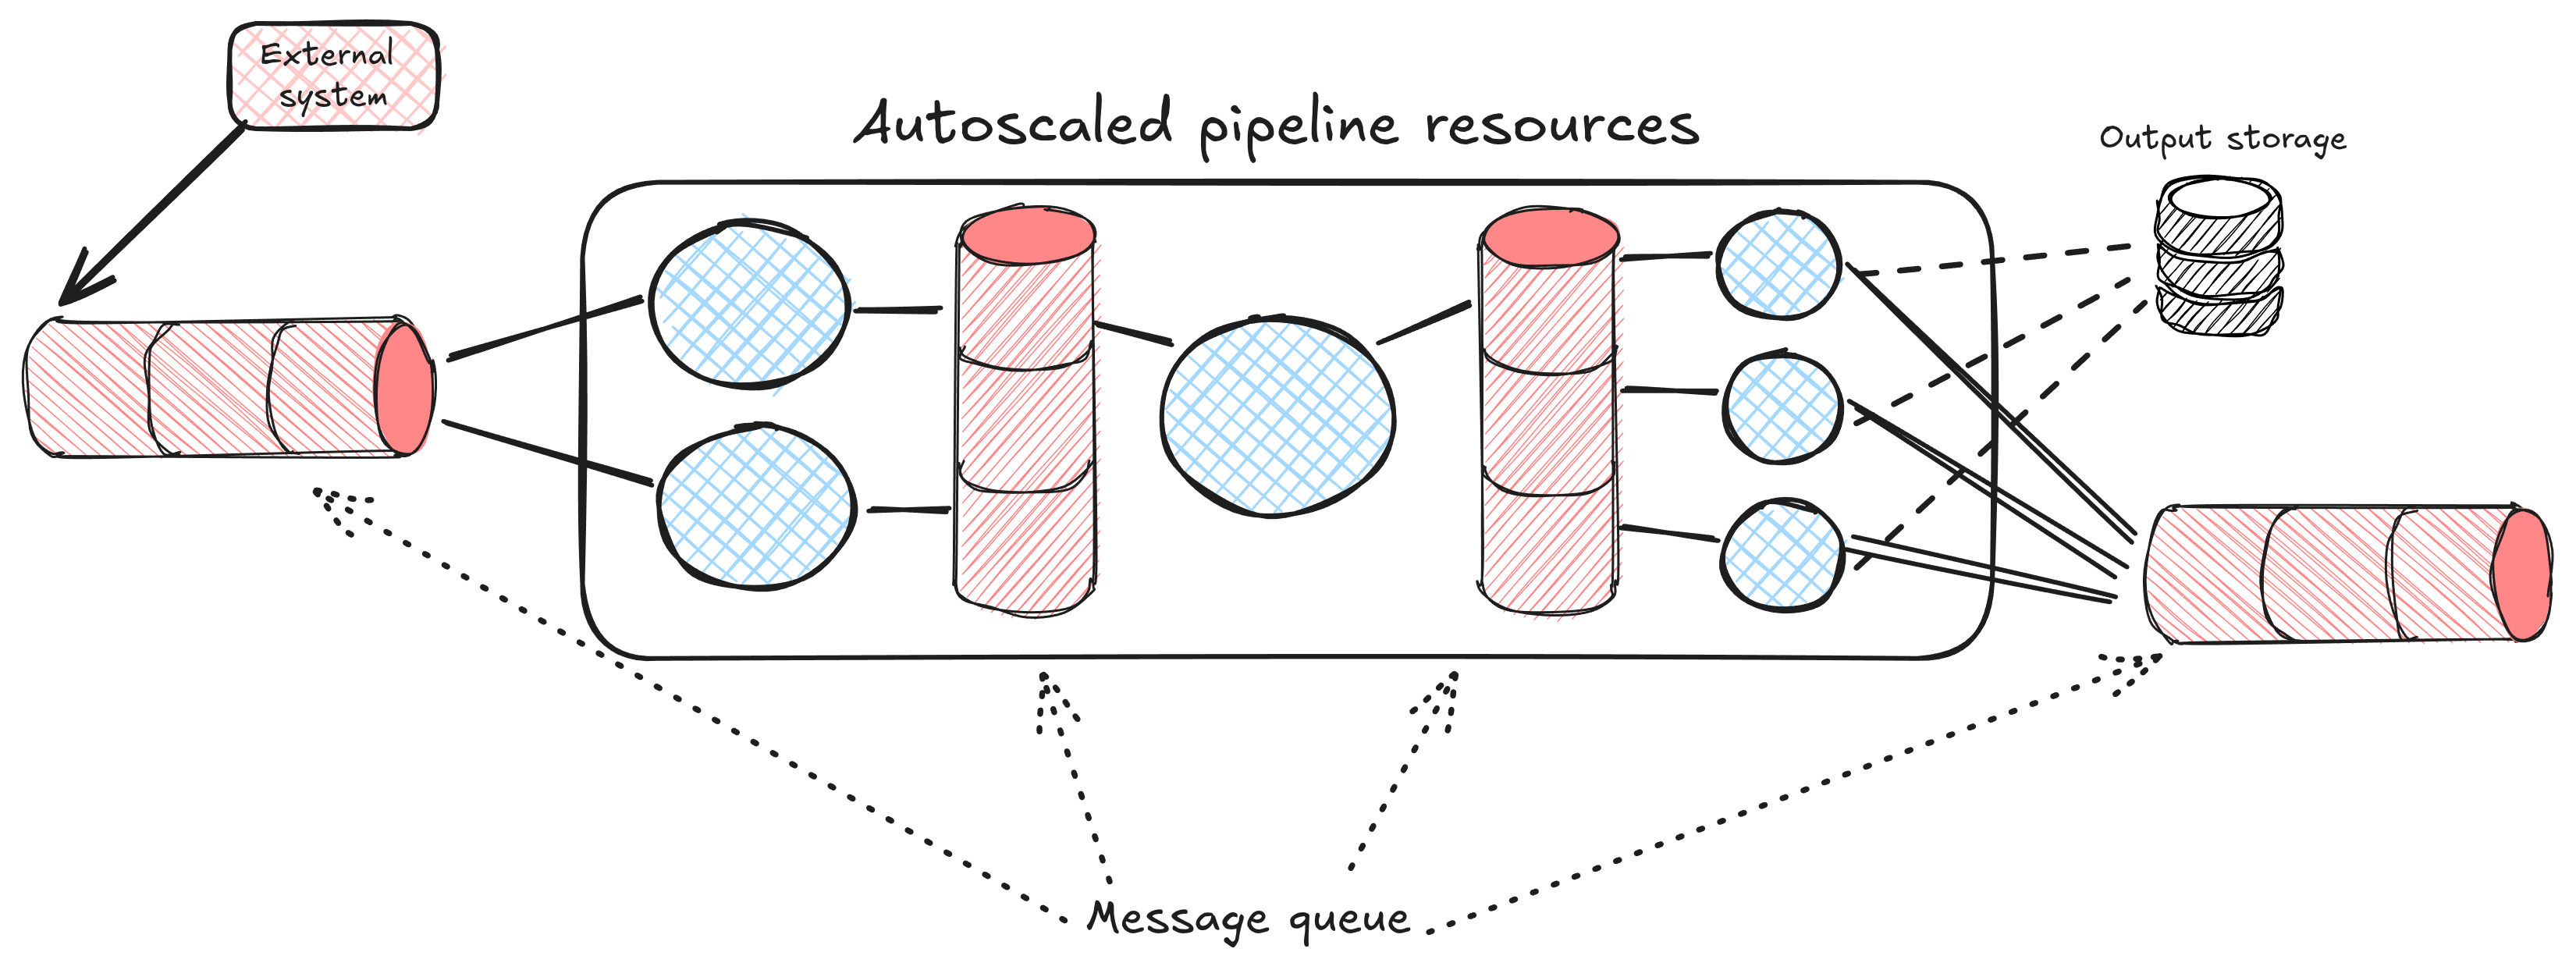
\includegraphics[width=0.8\textwidth]{images/stream-pipeline.png}
    \caption{\label{fig:stream-pipeline}Stream pipeline}
\end{figure}

\chapter{Implementation Part -- Storage}
\label{ch:impl_storage}

\section{Picture Store Requirements}\label{sec:picture_store_requirements}
The design and implementation of the storage infrastructure is driven by specific real-world constraints and needs specified by the company Recombee. The company specializes in AI-powered recommendation systems and search. To support advanced content-based recommendation and visual search, the system must ingest and retain massive datasets of raw product images. These images are used to compute vector embeddings and are later used in company products. The storage solution must not only serve as an archive but also provide high-performance access for machine learning pipelines.

To address the challenges of the Small File Problem and support the machine learning pipeline, the storage infrastructure must meet specific criteria. These requirements are divided into functional requirements (what the system must do) and non-functional requirements (how the system must perform).

\subsection{Functional Requirements}\label{sec:functional_requirements_storage}

\begin{itemize}
    \item \textbf{Small files, large amount} \\
    The system must efficiently store and retrieve binary files (images) with sizes ranging typically from 10 KiB to $\approx$1 MiB. The system must handle a large amount of these items without significant performance degradation.
    \item \textbf{Immutability (Write-Once-Read-Many)} \\
    Storage must prioritize read operations. Once an image is ingested, it is rarely updated. The system should be optimized for writing once and reading frequently. Updating existing data is not a required feature. Deletion is required, but its performance is not critical.
    \item \textbf{Flat addressability} \\
    Images must be identifiable and retrievable via a unique identifier (ID). It must not suffer from directory traversal like in POSIX systems.
    \item \textbf{Custom metadata} \\
    Each stored object needs to support custom metadata. Specified metadata may be used as an ID (address) for the stored object. It can maintain a mapping or integrate with an external index to locate these binary files by specific business keys.
    \item \textbf{Tunable or strong consistency} \\
    The system must provide strong consistency or guarantee Read-After-Write consistency. This ensures that once a file is successfully stored and acknowledged, it is immediately available for retrieval from any node in the cluster. No node should report missing data immediately after a successful write operation.
\end{itemize}

\subsection{Non-Functional Requirements}
\begin{itemize}
    \item \textbf{Fault Tolerance} \\
    The solution must be a Distributed File System (DFS) that tolerates node failures. The system must tolerate the failure of one replica of a stored item or of a node that stores data for that item.
    \item \textbf{Horizontal Scalability} \\
    The system must be capable of scaling out. It should allow for the addition of new storage nodes to the cluster to increase capacity and throughput without interruption of service.
    \item \textbf{Throughput for Batch Processing} \\
    The storage must support high parallel read throughput to feed offline ML jobs (e.g., batch processing) that compute embeddings effectively on large datasets.
    \item \textbf{Interface Compatibility} \\
    The system should provide an interface to access the data. POSIX interface is not required.
\end{itemize}

\section{SeaweedFS}
Based on the analysis of distributed storage solutions and the theoretical evaluation of storage solution implementations in Section \ref{sec:dfs_implementations} (not all were mentioned -- MinIO, RustFS), SeaweedFS was selected as the optimal solution for the image storage infrastructure (the problem addressed by the thesis). 
SeaweedFS was specifically optimized to handle a large number of small files and is based on the Haystack architecture, which was created for the same purpose as the motivation for this thesis.

The decision to choose SeaweedFS as the storage solution was highly influenced by experiences and case studies of projects and businesses that deal with similar needs. The decision is also supported by available benchmarks evaluating storage, especially object ones, focusing on the Small File Problem. The following sections point out three main benchmarks and studies.\footnote{Please be aware that presenting (not one's own) benchmarks is difficult to do correctly. Take those benchmarks just like examples -- for a complex understanding, dive into the mentioned studies directly.} 

\subsubsection*{Performance Evaluation of Object Storages}
The performance data presented in Table \ref{tab:bm1} are derived from the \textit{Performance Evaluation of Object Storages} report (2022) conducted by the NHR (National High Performance Computing) \cite{lackschewitz_performance_2022}. The benchmark used the S3Warp benchmark in Mixed mode\footnote{Designed and created by the MinIO project.}, specifically configured with a 4 KiB object size, to evaluate efficiency in handling large numbers of small files \cite{lackschewitz_performance_2022}. 

The tests were executed on nodes provided by \textit{NHR@Göttingen} (German High-Performance Computing Center). The results demonstrate that, for small-object workloads, critical storage system SeaweedFS performs well compared to both commercial and open-source alternatives in terms of IOPS and also bandwidth. \cite{lackschewitz_performance_2022}

\begin{table}[!ht]\centering
    \renewcommand{\arraystretch}{1.3}
    \begin{tabular}{r|r|r}
         Storage & Mixed IOPS \textit{[obj/s]}  & Mixed Bandwidth \textit{[MiB/s]} \\ \hline \hline
         SeaweedFS  &  58 836.57 & 137.89 \\
         Vast       &  36 897.36 & 84.45 \\
         Ceph       &  35 779.63 & 81.89 \\
         Oceanstor  &  31 023.44 & 72.71 \\
         MinIO      &  9 901.16  & 23.20 \\
    \end{tabular}
    \caption[Comparison of mixed workload performance]{Comparison of mixed workload performance (4 KiB objects) across different S3 storage systems.\cite{lackschewitz_performance_2022}}
    \label{tab:bm1}
\end{table}

\subsubsection*{Sandcrawler Proposal}
A 2020 proposal from the Sandcrawler project evaluated object storage solutions for handling large volumes of small PDF analysis files, revealing significant performance differences between MinIO and SeaweedFS. The report said that the existing MinIO implementation began to experience slowed insert rates after storing approximately 80 million objects. In contrast, the same benchmark on SeaweedFS demonstrated its scalability by successfully ingesting 200 million objects (about 550 GB), with constant insert times and utilizing only 400 MB of RAM. \cite{newbold_notes_2001}

\subsubsection*{Evaluation of Object Storage Performance using OStoreBench}
This study was created by researchers from the Institute of Computing Technology, Chinese Academy of Sciences, in collaboration with ByteDance \cite{kang_ostorebench_2020}. In this paper, they introduced new benchmark called OStoreBench. The primary motivation for developing OStoreBench was the inadequacy of existing industry-standard tools, which typically perform simple read/write operations without accounting for complex real-world variables such as request arrival patterns or diverse file size distributions.

OStoreBench evaluates systems by simulating critical paths from three distinct real-world application scenarios: \textit{Online Services} (latency-sensitive, primarily small files following a log-normal distribution), \textit{Big Data Analysis} (throughput-oriented, large files), and \textit{File Backup} (periodic uploads of small files similar to personal cloud storage).\cite{kang_ostorebench_2020}

The benchmark compared three storage systems: Ceph, OpenStack Swift, and SeaweedFS. The experiments revealed that SeaweedFS consistently outperformed the other systems in all three scenarios. In the latency-sensitive Online Service scenario, SeaweedFS achieved an average throughput of 10.8 MB/s, compared to Ceph (1.3 MB/s) and Swift (0.9 MB/s).\cite{kang_ostorebench_2020}

\section{Deployment}
The selected storage solution, SeaweedFS, was deployed within the Recombee infrastructure to validate its functionality and the requirements outlined in Section \ref{sec:picture_store_requirements}. 

The following text describes the storage deployment at a high level of abstraction. Concrete deployment can be seen in the provided media.
\subsection{Infrastructure and Hardware}
The storage cluster was deployed on four dedicated bare-metal servers. All nodes consist of NVMe SSD disks with storage organized by LVM.

Using NVMe drives is critical for this use case, as the "Small File Problem" often saturates mechanical drives (HDDs) due to high IOPS requirements, even if throughput bandwidth is not fully utilized.
\subsection{Orchestration with Puppet Bolt}
To ensure the deployment process was reproducible and aligned with Recombee's operational standards, the installation and configuration were orchestrated with Puppet Bolt.

This technology was chosen to maintain the consistency of the Puppet technology already used for managing the provided servers. At the time of implementation, no official or community-supported Puppet module for SeaweedFS existed on the Puppet Forge. 

To address this, a custom lightweight Puppet module was developed specifically for this thesis. This module focuses on booting up the necessary cluster components -- downloading binaries, configuring systemd services, and applying basic configuration files. While currently scoped to bootstrap the cluster for this implementation, the module is designed to expand into a fully featured, public module for the Puppet Forge in the future.

\subsection{Cluster Topology}
The deployed SeaweedFS cluster consists of multiple components that provide a fully functional solution that meets the requirements for such storage. The Master server, which is an essential storage component, is deployed as a systemd service. This service is deployed with a single replica that lacks HA. The Master server allows HA setup thanks to the Raft LE algorithm, which elects the leader among distributed instances. The architecture of the Master component limits the ability to run multiple replicas and perform load balancing between them. This limitation should not be a problem as pointed out in the above-mentioned studies. Official documentation points out that it is considered not a problem to run just one replica even for large deployment \cite{seaweedfs_seaweedfs_2024} \footnote{For more information, navigate to documentation section Production Setup.}.

Volume services are run on each node. Those services are responsible for the role of the data plane in the cluster. Each volume is aware of its placement (server, datacenter, rack), enabling data replication based on specified QoS. Volume servers run on LVM storage, with NVMe SSD disks. The chosen filesystem for the Volume server is XFS, which is recommended by SeaweedFS Wiki and is described as the most performant for the Haystack solution. \cite{seaweedfs_seaweedfs_2024, beaver_finding_2010} 

Filer service is a component deployed to satisfy functional requirements specified in Section \ref{sec:functional_requirements_storage}. Filer is (not essential for SeaweedFS) a service that manages simple metadata about stored blobs. It allows storage to act as POSIX storage by introducing (artificial) paths to stored blobs. Thanks to Filer, it is possible to list and access blobs as if they were stored at a specified path or URL. Filer is deployed as a standalone systemd service connected to the PostgreSQL database for persistent storage.

Among specified components, the deployment includes several services specifically for management and monitoring. Admin UI provides a graphical interface for the cluster. Worker service is used to automate background maintenance and asynchronous tasks. For observability, SeaweedFS exposes native metrics to a Prometheus instance, which are displayed in Grafana dashboard for visualization of cluster health and performance. This monitoring stack is architected to support future automated alerting extensions.

\chapter{Implementation Part -- Pipeline}\label{ch:impl_pipeline}

The objective of the thesis is to design and build a reliable, high-throughput streaming data processing pipeline for image processing, specifically embedding computation. The pipeline is intended to be used as an internal subsystem of the Recombee infrastructure, enabling businesses to offer new products. The system must download raw images from the internet, process them, and store them in internal storage. After successful storage, the pipeline computes the image representation and outputs it as the result.

\section{Pipeline Solution Architecture}
To meet the requirements of a high-performance and scalable stream pipeline, the pipeline relies on a Kafka message broker. The broker serves as a task queue (input) for the pipeline and its jobs and as a communication layer between pipeline stages. Kafka is designed to handle massive throughput and offers low-latency data feeds, which are essential for building a streaming pipeline that must maintain high throughput while providing low latency. Due to its distributed architecture, it provides concurrent access without blocking, enabling the pipeline to scale horizontally during peak requests. Kafka persists events on disk and replicates them across a cluster of brokers. This ensures that processing tasks remain durable and available even in the case of hardware failure. Kafka was chosen as the backbone of the pipeline because it serves as the interface through which the Recombee infrastructure communicates with other services, enabling easy integration with existing systems. Any other message queue that meets the specified criteria (scalability, durability, concurrent access) could be used in the pipeline.  

The pipeline itself follows a distributed, modular architecture. By decomposing the end-to-end process into discrete logical units (jobs), the system can independently scale computationally intensive tasks and provide clear checkpoints for failure recovery. This modularity ensures that a bottleneck in image downloading does not stall the embedding computation, and vice versa.

The implementation is structured into two primary components (Downloader and Embedder) that communicate via similarly named Kafka topics. The pipeline also uses an Image Reactor component to log and maintain the entire index of available images.

\subsubsection{Downloader}
The Downloader is a concurrent application written in Go that connects external data sources with internal storage. To ensure high availability and horizontal scalability, the service is partitioned into two decoupled layers: the Ingestion Layer and the Worker Pool.

\paragraph{Ingestion and Rebalancing} \mbox{} \\
The first layer manages a Kafka consumer that fetches tasks from the downloader topic and forwards them into the internal (Go channel) queue. By decoupling message ingestion from the actual download process, the service can perform online autoscaling and immediate consumer rebalancing. This ensures that even during heavy I/O operations, the service remains responsive to Kafka’s protocol, allowing for seamless distribution of the workload across new instances.

\paragraph{Concurrent Worker Pool} \mbox{} \\
The second layer consists of a pool of independent workers that process images from the internal queue. Each worker performs the following operations:
\begin{itemize}
    \item \textbf{Downloading:} Downloads an image from the internet to memory.
    \item \textbf{Metadata extraction:} Extracts metadata of the image (size, format, hash) from the image.
    \item \textbf{Storage:} Uploads the image to internal image storage and separated metadata storage (Image Reactor -- see below).
    \item \textbf{Notification:} After all successful operations, the job is published in the embedding topic to trigger the embedding computation.
\end{itemize}

Any failure during image processing is reported to the Image Reactor. By centrally logging these errors, the system enables subsequent examination and manual or automated retries. This reporting mechanism ensures that individual task failures do not stall the pipeline, allowing workers to remain highly available for subsequent tasks.

\subsubsection{Image Reactor}
The Image Reactor is an application that stores application metadata of downloaded images. It is a Python REST API designed to decouple physical storage locations from application-specific metadata. By acting as a specialized catalog, it provides the abstraction layer necessary to satisfy business requirements without placing additional load on the primary image storage system. Decoupling application and storage metadata is a concept proposed by the Haystack paper \cite{brewer_cap_2012}. While raw image data reside in a dedicated image store, the Reactor tracks associated attributes, such as resolution, format, and business-specific tags, that are essential for product usage.

The Reactor persists metadata in a dedicated and replicated PostgreSQL database, providing transactional guarantees for every record. The application is designed to be stateless, enabling horizontal scalability and high availability. The implementation employs a concurrency pattern to maximize throughput while keeping resource requirements, such as CPU and memory, low.

The Reactor also records all errors that occur during the data processing pipeline. It can be understood as a central logging system for pipeline failures. When a worker experiences any failure while processing the image, the Reactor records this failure. By logging these errors centrally, the system provides a clear mechanism for evaluating failed jobs and triggering manual or automated retries based on specific business logic. This ensures that individual task failures are isolated and do not stall the high-throughput processing of the remaining queue.

\subsubsection{Embedder}
The Embedder is the final component in the data processing pipeline. The application transforms raw image data into the corresponding embedding vector representation. Its architecture is similar to the Downloader: it consumes tasks from a dedicated Kafka topic. The Kafka message includes the image path in the internal image storage, along with the data required for correct image transformation. Similar to the Downloader, the Embedder can run multiple computations in parallel if needed. The ability to consume messages from Kafka and images from internal data storage simultaneously makes the Embedder horizontally scalable.  

\section{Pipeline}
The complete pipeline is a distributed system comprising multiple specialized components, including the Downloader, the Embedder, and the Image Reactor. Each component serves a strictly defined purpose within the data processing lifecycle, enabling the system to be precisely tuned to specific requirements. By decoupling these stages via Kafka topics, the pipeline enables scaling based on the required workload, a key objective of any streaming pipeline. For a complete overview of the system architecture and the data flow between these components, refer to the diagram in Figure \ref{fig:dt-pipeline}.

\begin{figure}[h!t]
    \centering
    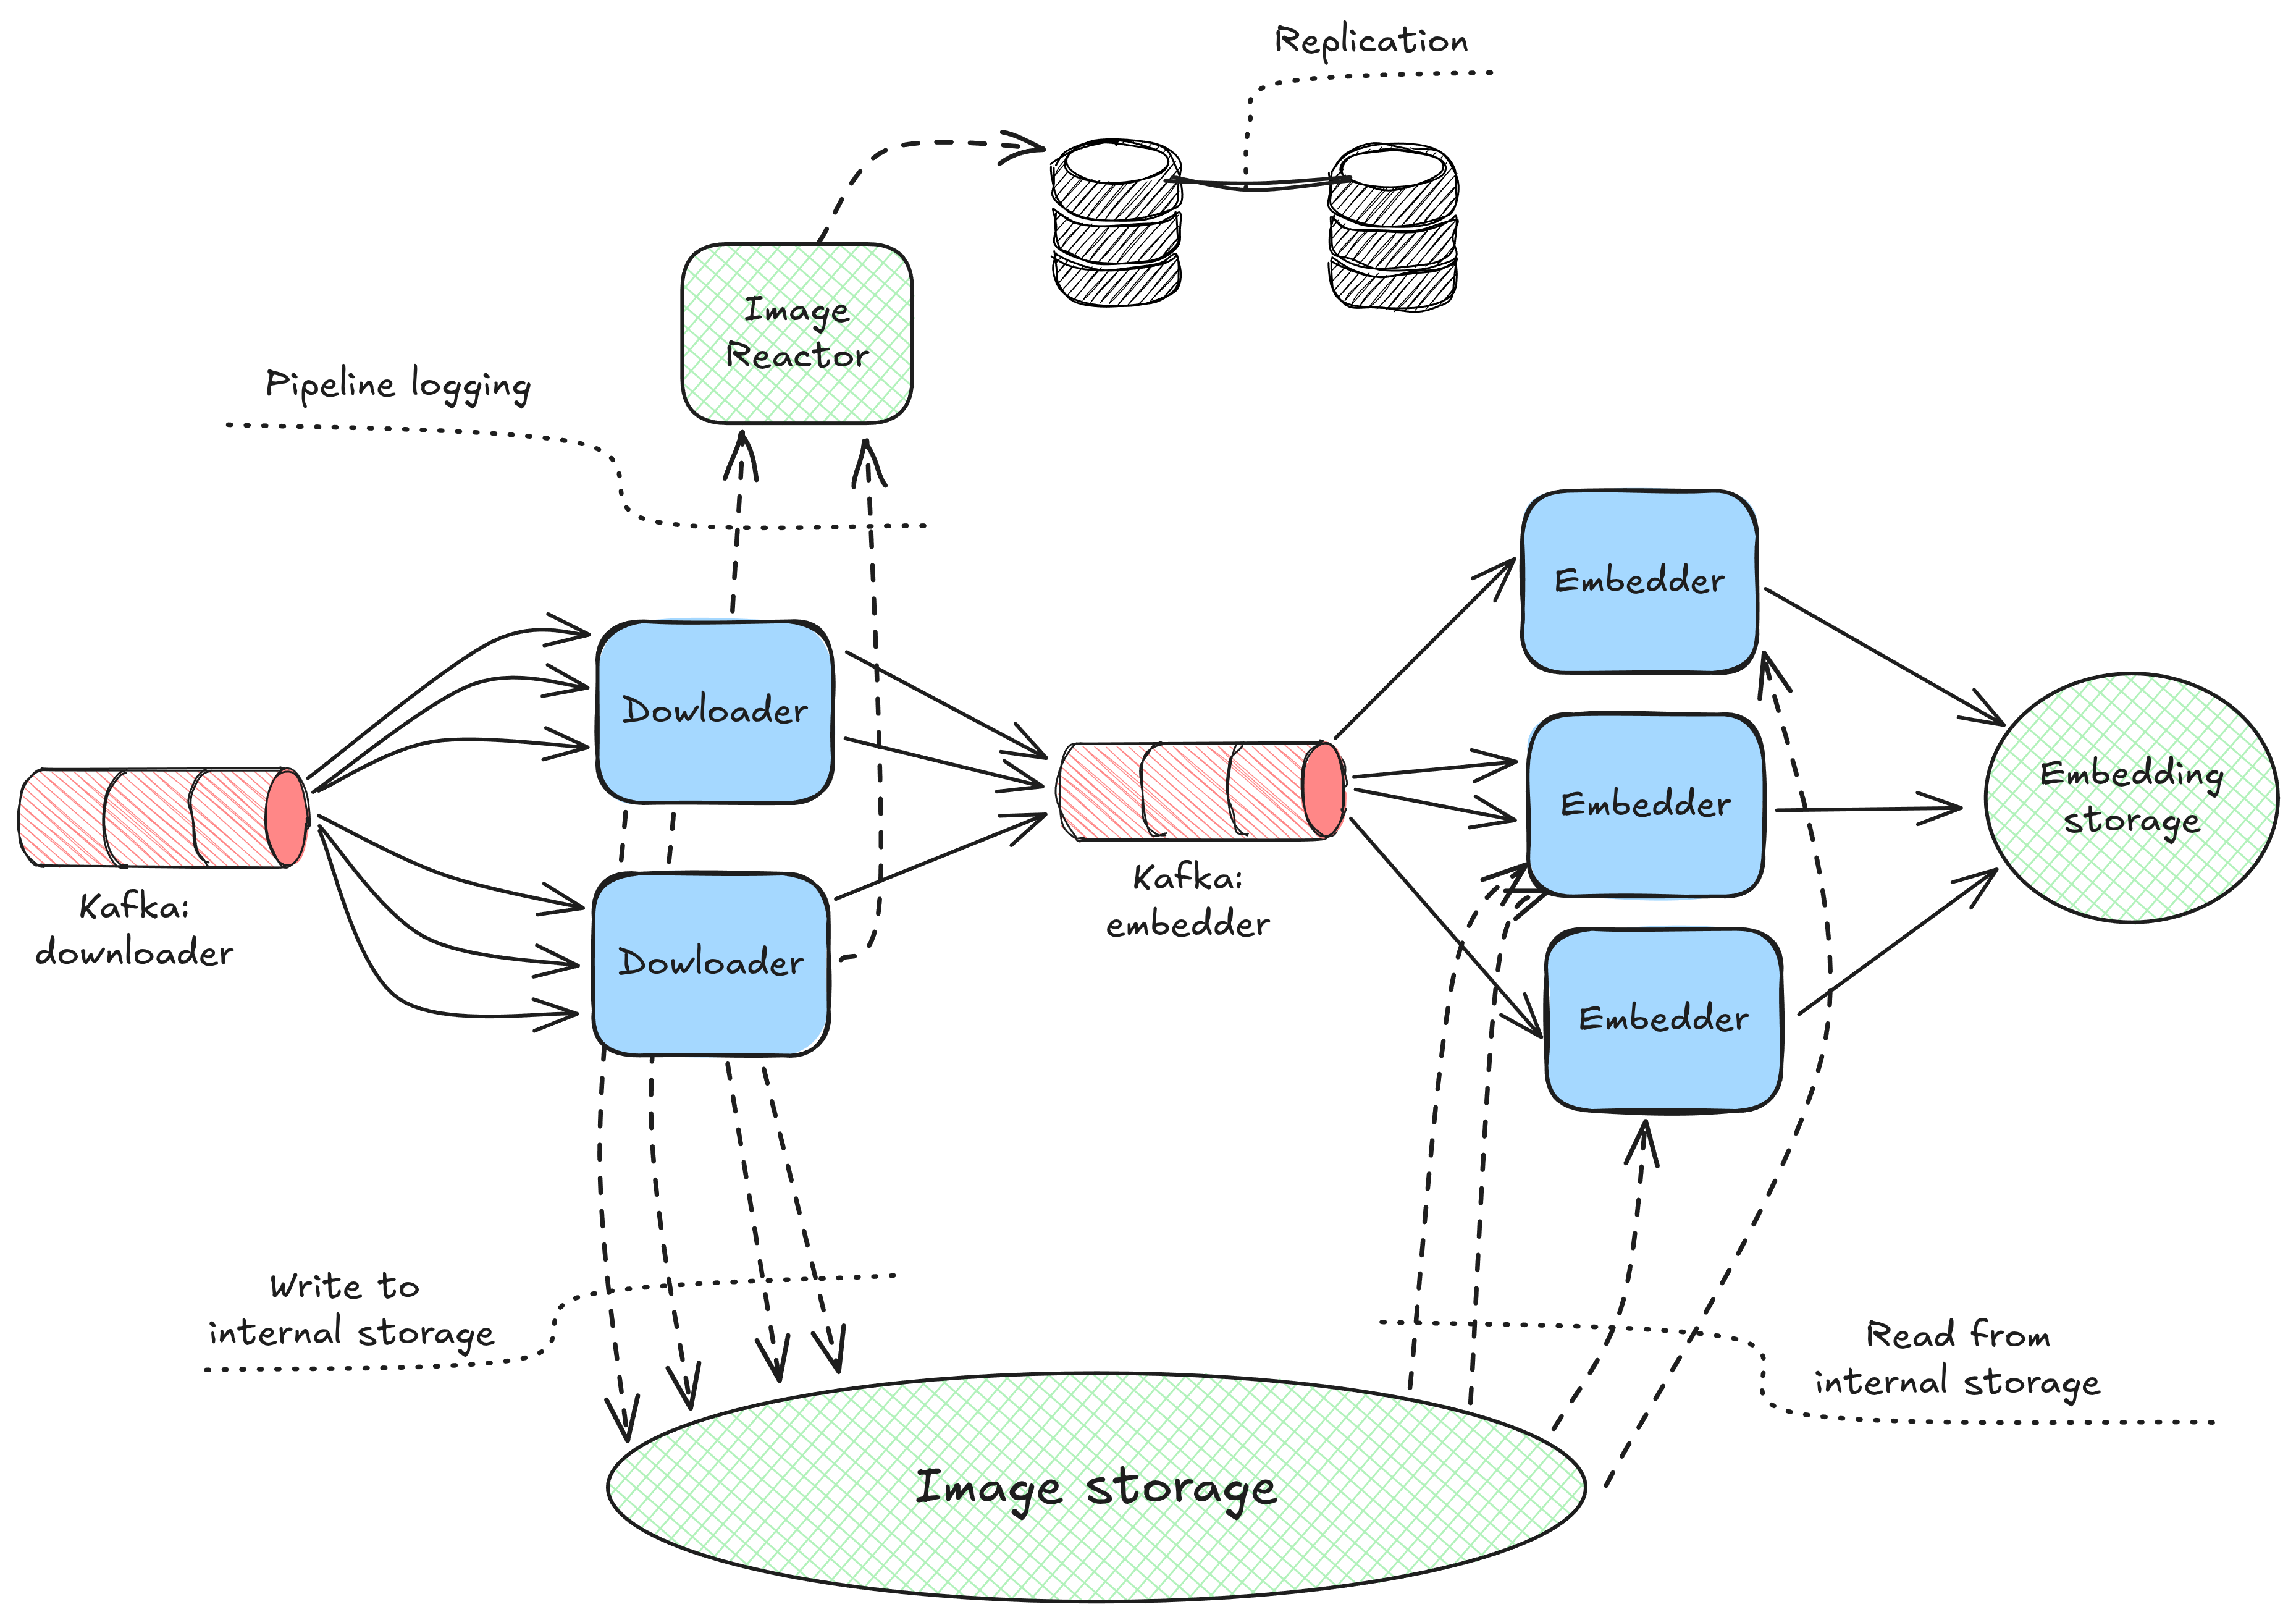
\includegraphics[width=0.9\textwidth]{images/dt-pipeline.png}
    \caption{\label{fig:dt-pipeline}Data processing pipeline architecture}
\end{figure}

\section{Deployment and Orchestration}
The components and pipeline described in the previous sections constitute the system's logical architecture. However, for the pipeline to function within a production environment, the setup must guarantee High Availability (HA) and scalability. Such properties can only be achieved by deploying the system across multiple nodes, with operations distributed across them.

There are several ways to achieve this orchestration over multiple nodes. For pipeline deployment, Kubernetes was chosen. Kubernetes is a container orchestrator that provides a way (almost standardized \cite{pope_why_2019}) to deploy applications. In addition to deployment, it is designed to handle service discovery, scheduling, networking, storage, and other required services. This makes it suitable for deploying the designed pipeline.

The Kubernetes orchestrator provides building blocks for building a pipeline that is HA, fault-tolerant, and supports scheduling and load balancing. To make the pipeline truly streamlined, automatic dynamic scheduling is needed for pipeline components. While automatic dynamic scheduling is not part of the core Kubernetes capabilities, it can be added through its extensible architecture. To enable automatic scalability, KEDA is used.

\subsection{Autoscaling}
KEDA (Kubernetes Event-Driven Autoscaling) is a component that extends Kubernetes to provide event-based scaling. KEDA enables the cluster to respond directly to external events and scale Kubernetes objects accordingly. It is designed to work natively with the Kubernetes API and can scale Deployments (stateless applications), StatefulSets (stateful applications), and Jobs (one-time tasks).

KEDA uses scaler plugins that provide event-based triggers. These scalers act as monitors of external services, such as databases and messaging queues. By monitoring these services, KEDA can trigger scaling actions based on the actual state of the data in these systems. One of those plugins is the Kafka Scaler. The Kafka Scaler enables autoscaling of Kubernetes components based on consumer lag. Kafka Scaler monitors the number of unread messages in a specific topic. If the lag increases, KEDA proactively schedules additional pods to handle a higher workload required to consume the Kafka topic. This ensures the pipeline is down-scheduled to minimal resources while remaining available in case no or low processing is required. On the other hand, when higher processing performance is required, KEDA can automatically horizontally scale the pipeline stages.

\vspace{1.5em}
The complete deployment example, including the code for each mentioned component, is provided in the attached media. 

\section{Properties of Pipeline}
The architecture of the designed pipeline, its deployment, and the implementation of its components meet the requirements of a streaming AI image-processing pipeline. The following list describes the implementation's specific technical properties.

\begin{itemize}
    \item \textbf{High Availability} \\
    All components in the pipeline, including Kafka and storage, are designed to offer high availability. The only component that does not fully support HA is PostgreSQL. Due to replication, it should be possible to switch to the replica if needed; however, this may result in partial data loss and a brief outage. Since the Image Reactor does not directly affect the pipeline, it should not affect the pipeline's availability.
    \item \textbf{Scalability and Throughput} \\
    The pipeline is designed to be horizontally scalable. Supportive storage may introduce limitations in scalability. PostgreSQL is designed to be vertically scalable rather than horizontally. To enable horizontal scalability of the Reactor's persistent layer, an alternative database technology should be considered. The Master server of SeaweedFS is the only component that is not horizontally scalable (for write) in the SeaweedFS deployment. During the design of the pipeline and the writing of the thesis, no evidence of its performance deficiencies was found. The last component that can influence scalability is Kafka. Kafka limits the number of consumers to the number of partitions used in the topic. It is a known limitation that is rarely encountered. To enable the pipeline to scale beyond the number of partitions in Kafka topics, a Consumer Proxy pattern can be used \cite{yang_enabling_2021}.
    \item \textbf{Monitoring} \\
    Because the streaming pipeline's internal processes are difficult to validate in production, all components expose metrics to enable visualization of the processes occurring within them. Pipeline components expose Prometheus metrics that are scraped by the Prometheus instance and displayed in the Grafana dashboard. The metric setup, including the Grafana dashboard, is included in the attached media.
\end{itemize}

The designed pipeline architecture and its specific implementation meet the requirements for high-throughput streaming AI image processing. During testing, no major problems were identified, and the system functioned as expected. The pipeline contains components that could limit its ability to scale horizontally, but these limitations are known and may be mitigated by the proposed improvements, in case such limits are met.
\chapter{Conclusion}
The primary objective of this thesis was to design and implement a scalable, on-premise infrastructure capable of gathering, processing, and storing large-scale image datasets for machine learning applications. Based on the analysis of distributed storage solutions and the practical deployment within the Recombee infrastructure, the project successfully addressed the small file problem by utilizing SeaweedFS. This architecture, inspired by Facebook’s Haystack, proved to be highly effective at reducing metadata overhead by grouping small images into larger volumes and maintaining indexes in fast memory. Testing of this storage implementation identified no major problems, and the system functioned as expected. However, it is important to note that while the evaluated benchmarks demonstrate superior performance on small-object workloads, they do not necessarily account for all complex variables or potential issues that may arise under different large-scale real-world workloads.

The implemented data processing pipeline successfully realized a hybrid stream-processing model that combines the low latency of online systems with the high throughput of offline batch systems. By leveraging Kafka as a message broker for inter-stage communication and Kubernetes for orchestration, the system achieved a high degree of modularity and fault tolerance. The use of KEDA for event-driven autoscaling ensured that pipeline components like the Downloader and Embedder can scale horizontally in response to consumer lag, optimizing resource efficiency during periods of low activity while maintaining high throughput during peak loads. The modular approach ensures that specific computational bottlenecks, such as intensive embedding calculations, do not stall the ingestion of new data.

The presented solution architecture is effective for building data processing pipelines with storage nodes optimized for small files. The design focuses primarily on small binary files and automated resource allocation. Its results can be applied to tasks with similar requirements, such as managing e-commerce platforms or storing social media photos. To further share the practical findings of this implementation, the deployment in production use of the work will be documented in a blog post, which will present detailed performance results from the production environment.
 % include `text.tex' from `text/' subdirectory

\appendix\appendixinit % do not remove these two commands

\chapter{Screenshots from deployment}

\begin{figure}[ht]
    \centering
    % This makes a box of 0pt width and puts the image in the center of it
    \makebox[\textwidth][c]{
        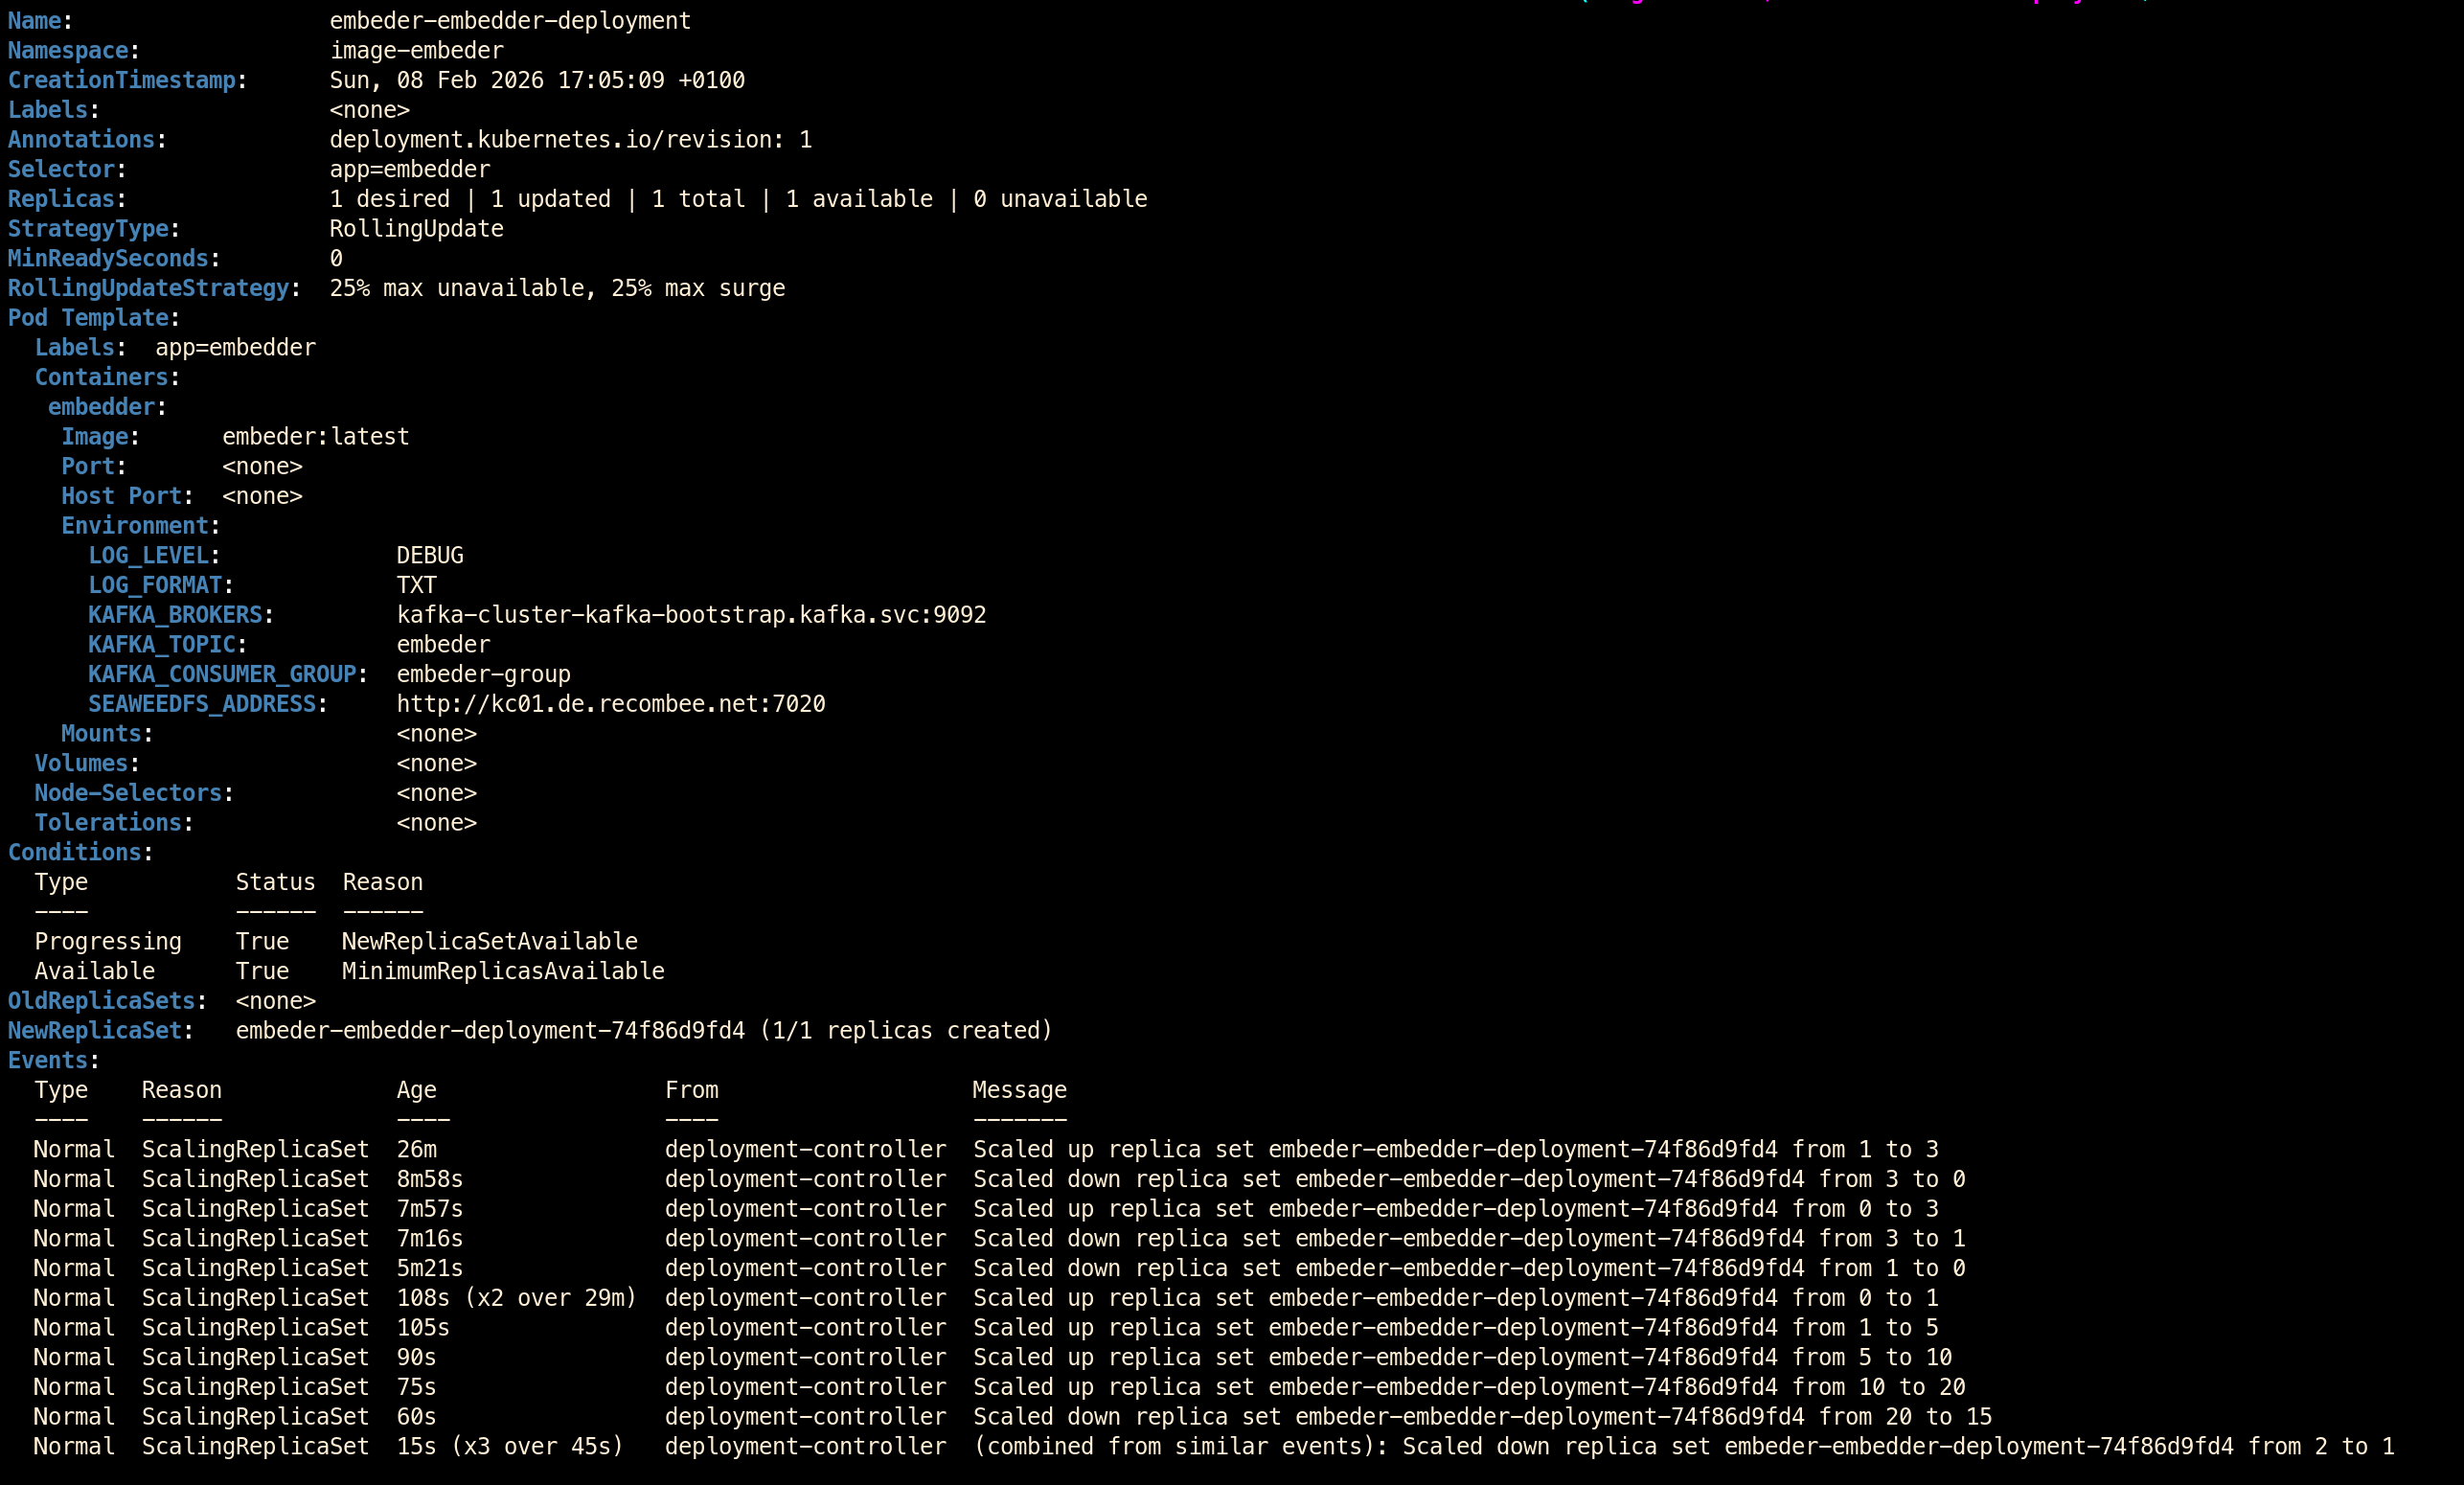
\includegraphics[width=0.85\paperwidth]{images/appendix/scalling.png}
    }
    \caption[Deployment scaling example]{Deployment scaling example. The screenshot contains events (bottom of the figure) of scaling the embedder component.}
\end{figure}


\begin{figure}[ht]
    \centering
    % This makes a box of 0pt width and puts the image in the center of it
    \makebox[\textwidth][c]{
        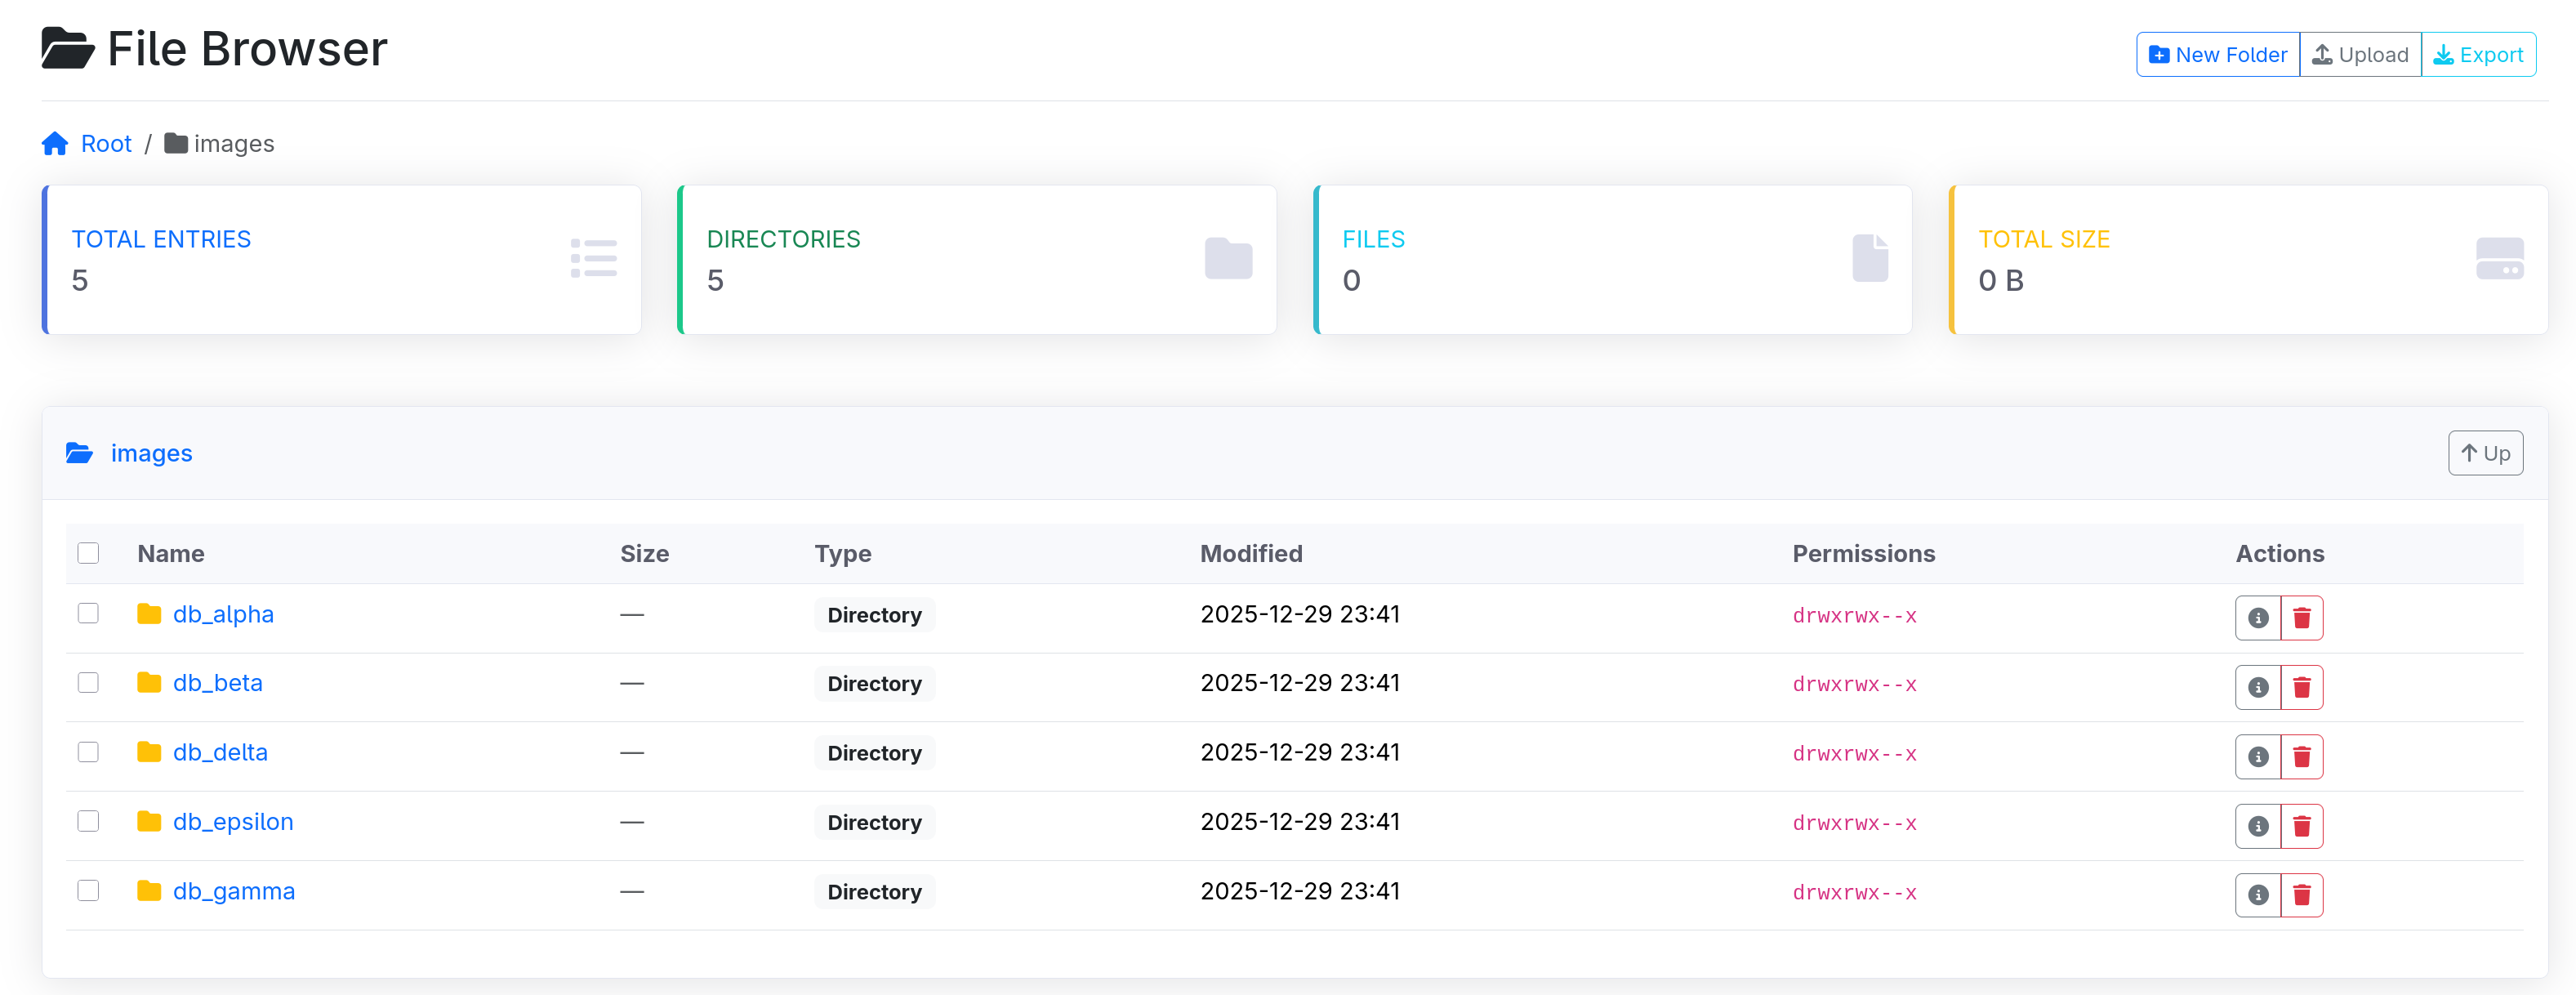
\includegraphics[width=0.85\paperwidth]{images/appendix/image.png}
    }
    \caption[Filler UI]{Filler UI. Web UI for interacting with filer. The web interface can be used to list, upload, delete files, and manage basic storage metadata.}
\end{figure}



\begin{figure}[ht]
    \centering
    % This makes a box of 0pt width and puts the image in the center of it
    \makebox[\textwidth][c]{
        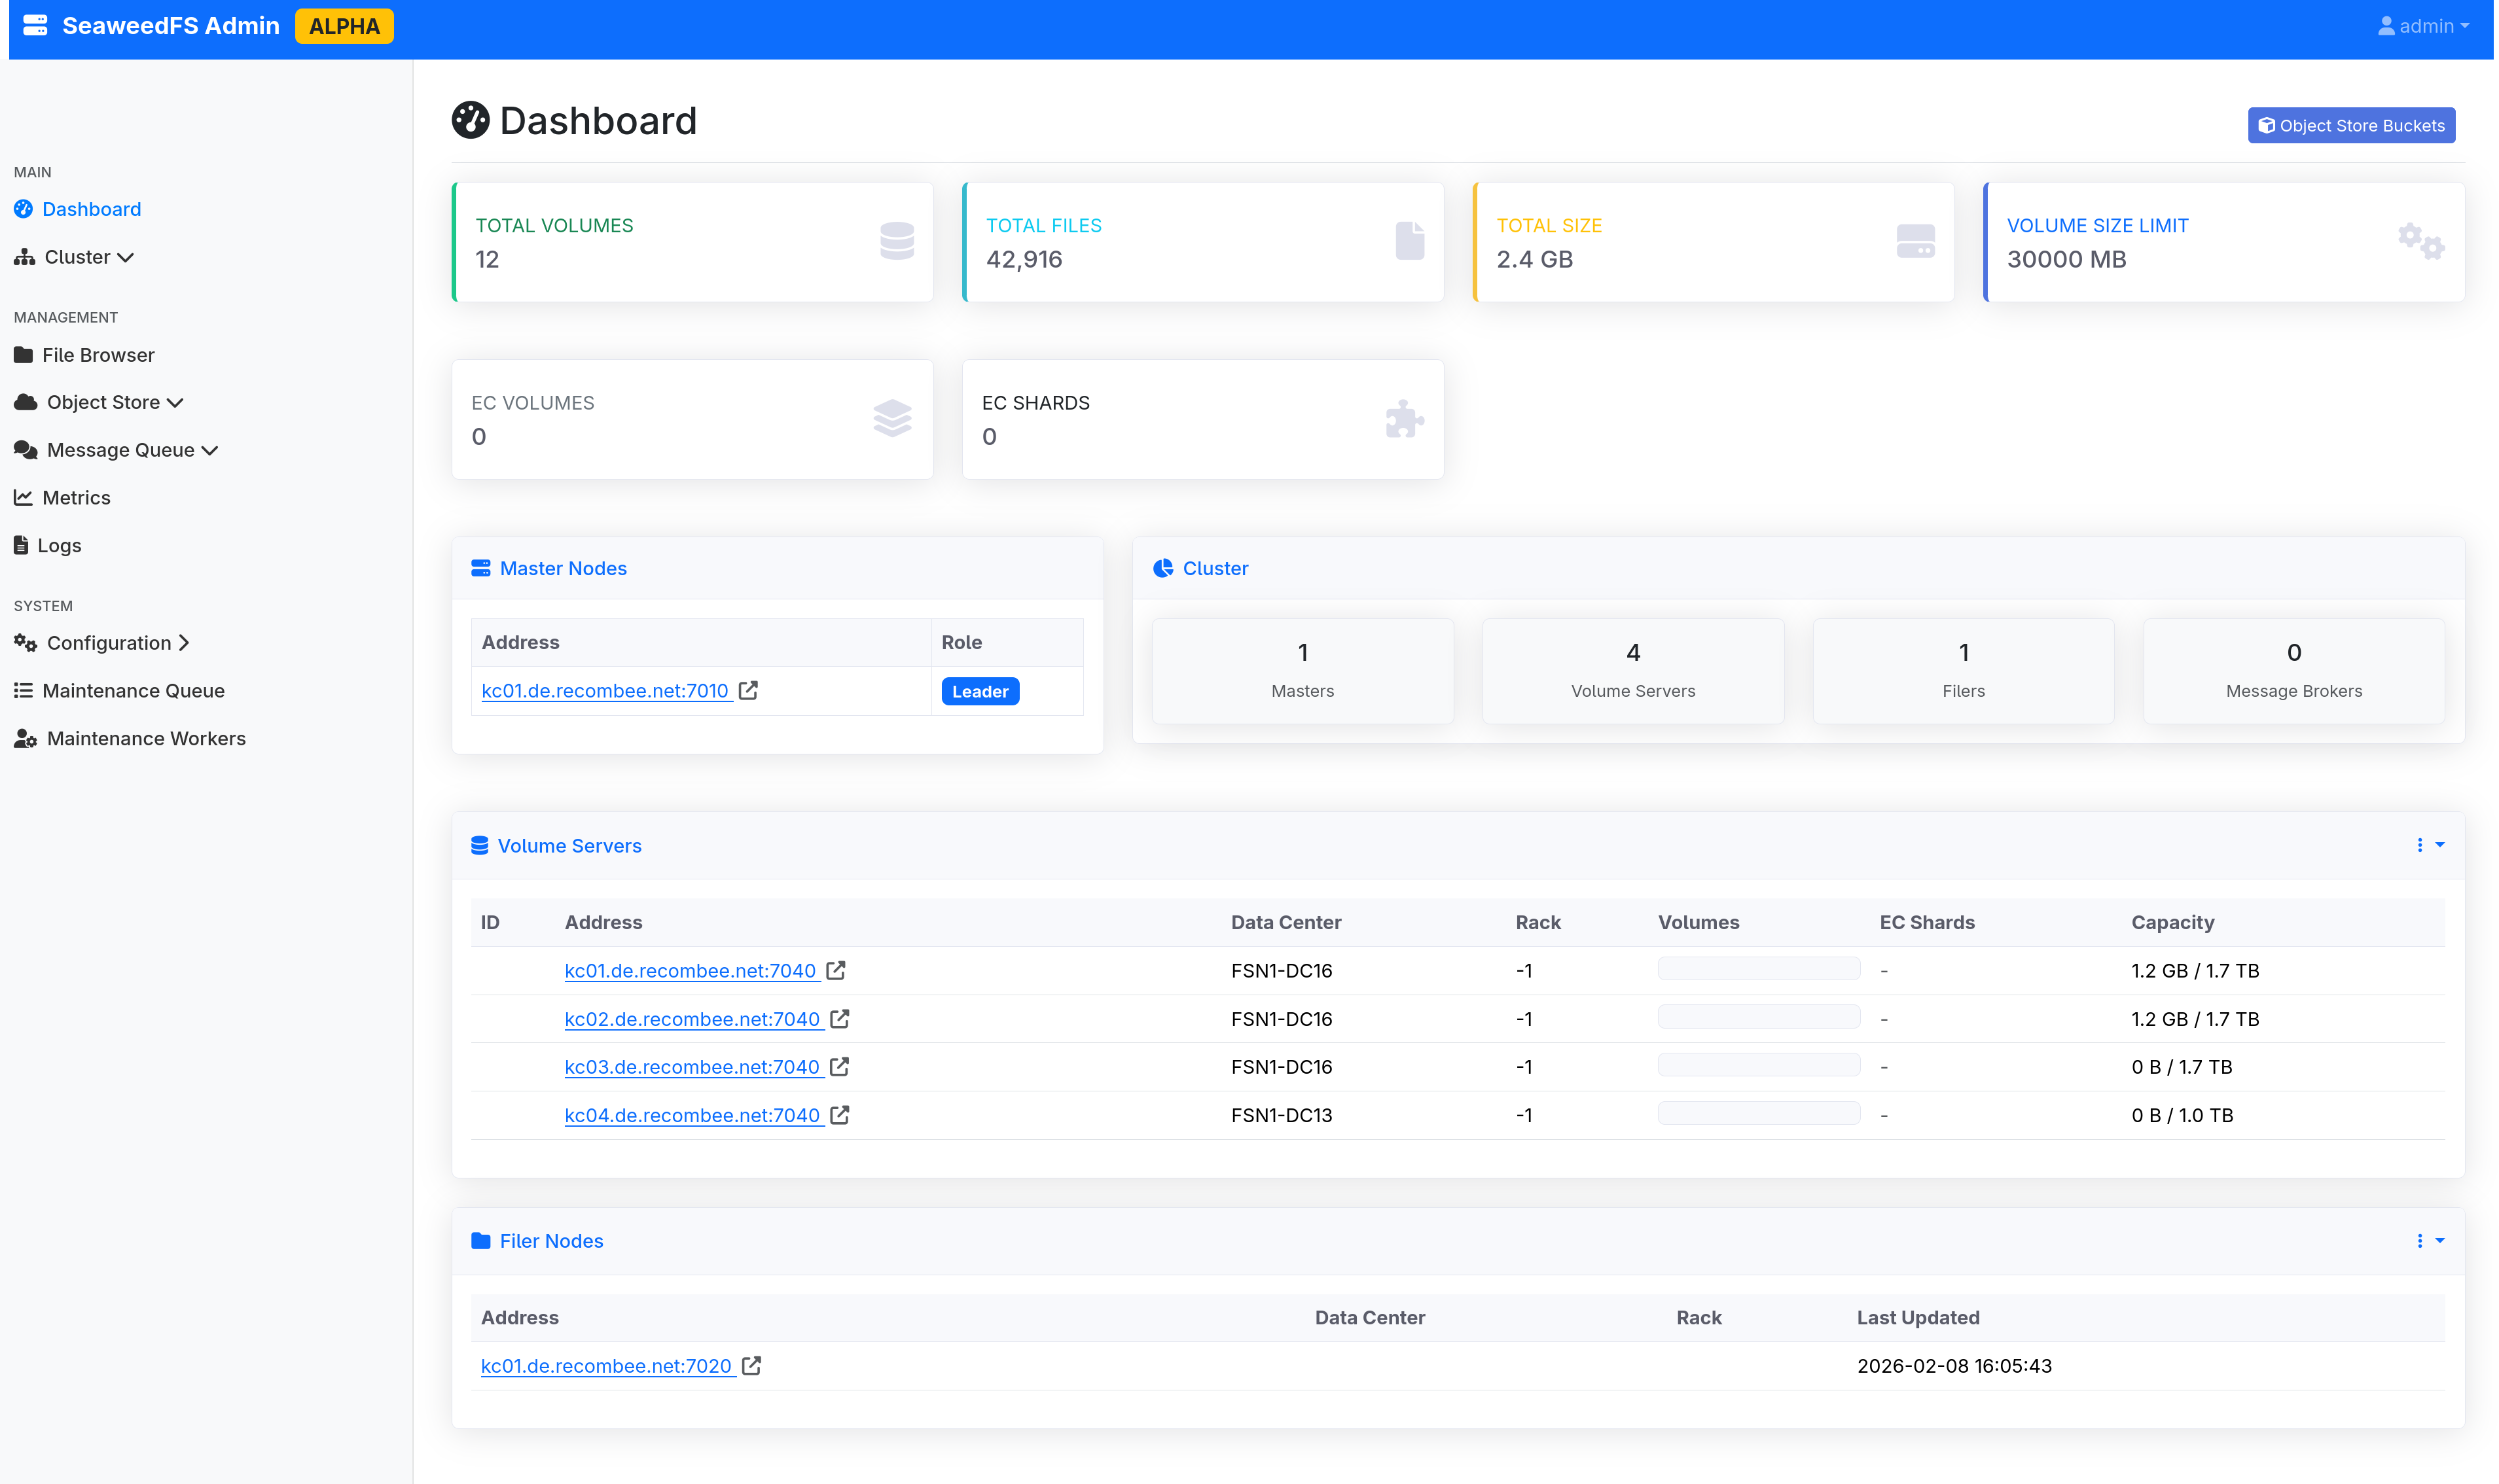
\includegraphics[width=0.85\paperwidth]{images/appendix/seaweed-API.png}
    }
    \caption{SeaweedFS admin UI}
\end{figure}


\begin{figure}[ht]
    \centering
    % This makes a box of 0pt width and puts the image in the center of it
    \makebox[\textwidth][c]{
        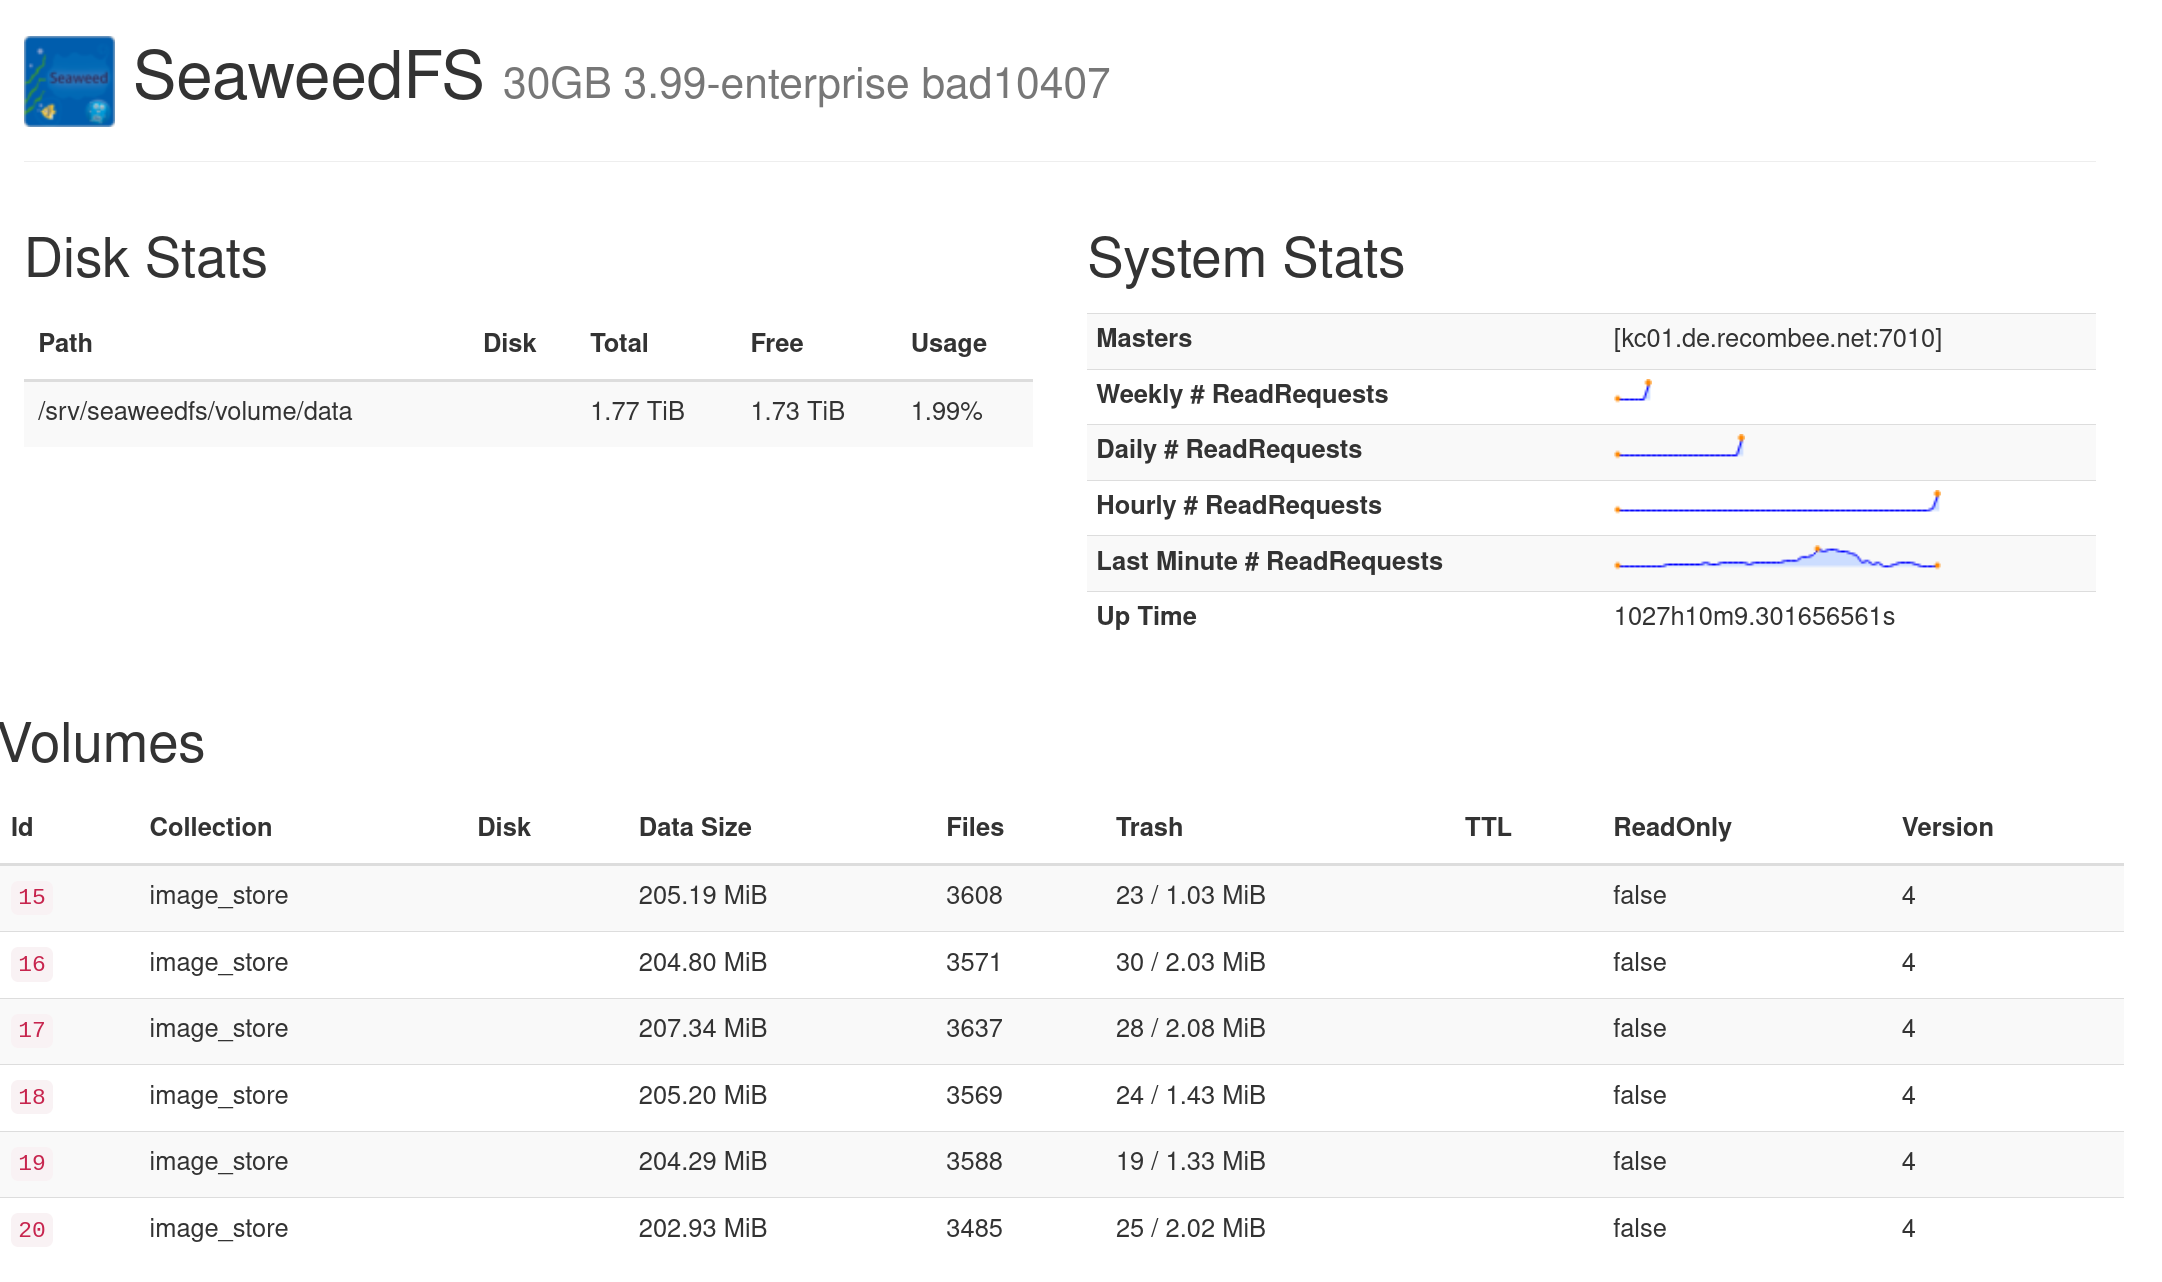
\includegraphics[width=0.85\paperwidth]{images/appendix/wolumeserverUI.png}
    }
    \caption{Volume server web UI}
\end{figure}

\begin{figure}[ht]
    \centering
    % This makes a box of 0pt width and puts the image in the center of it
    \makebox[\textwidth][c]{
        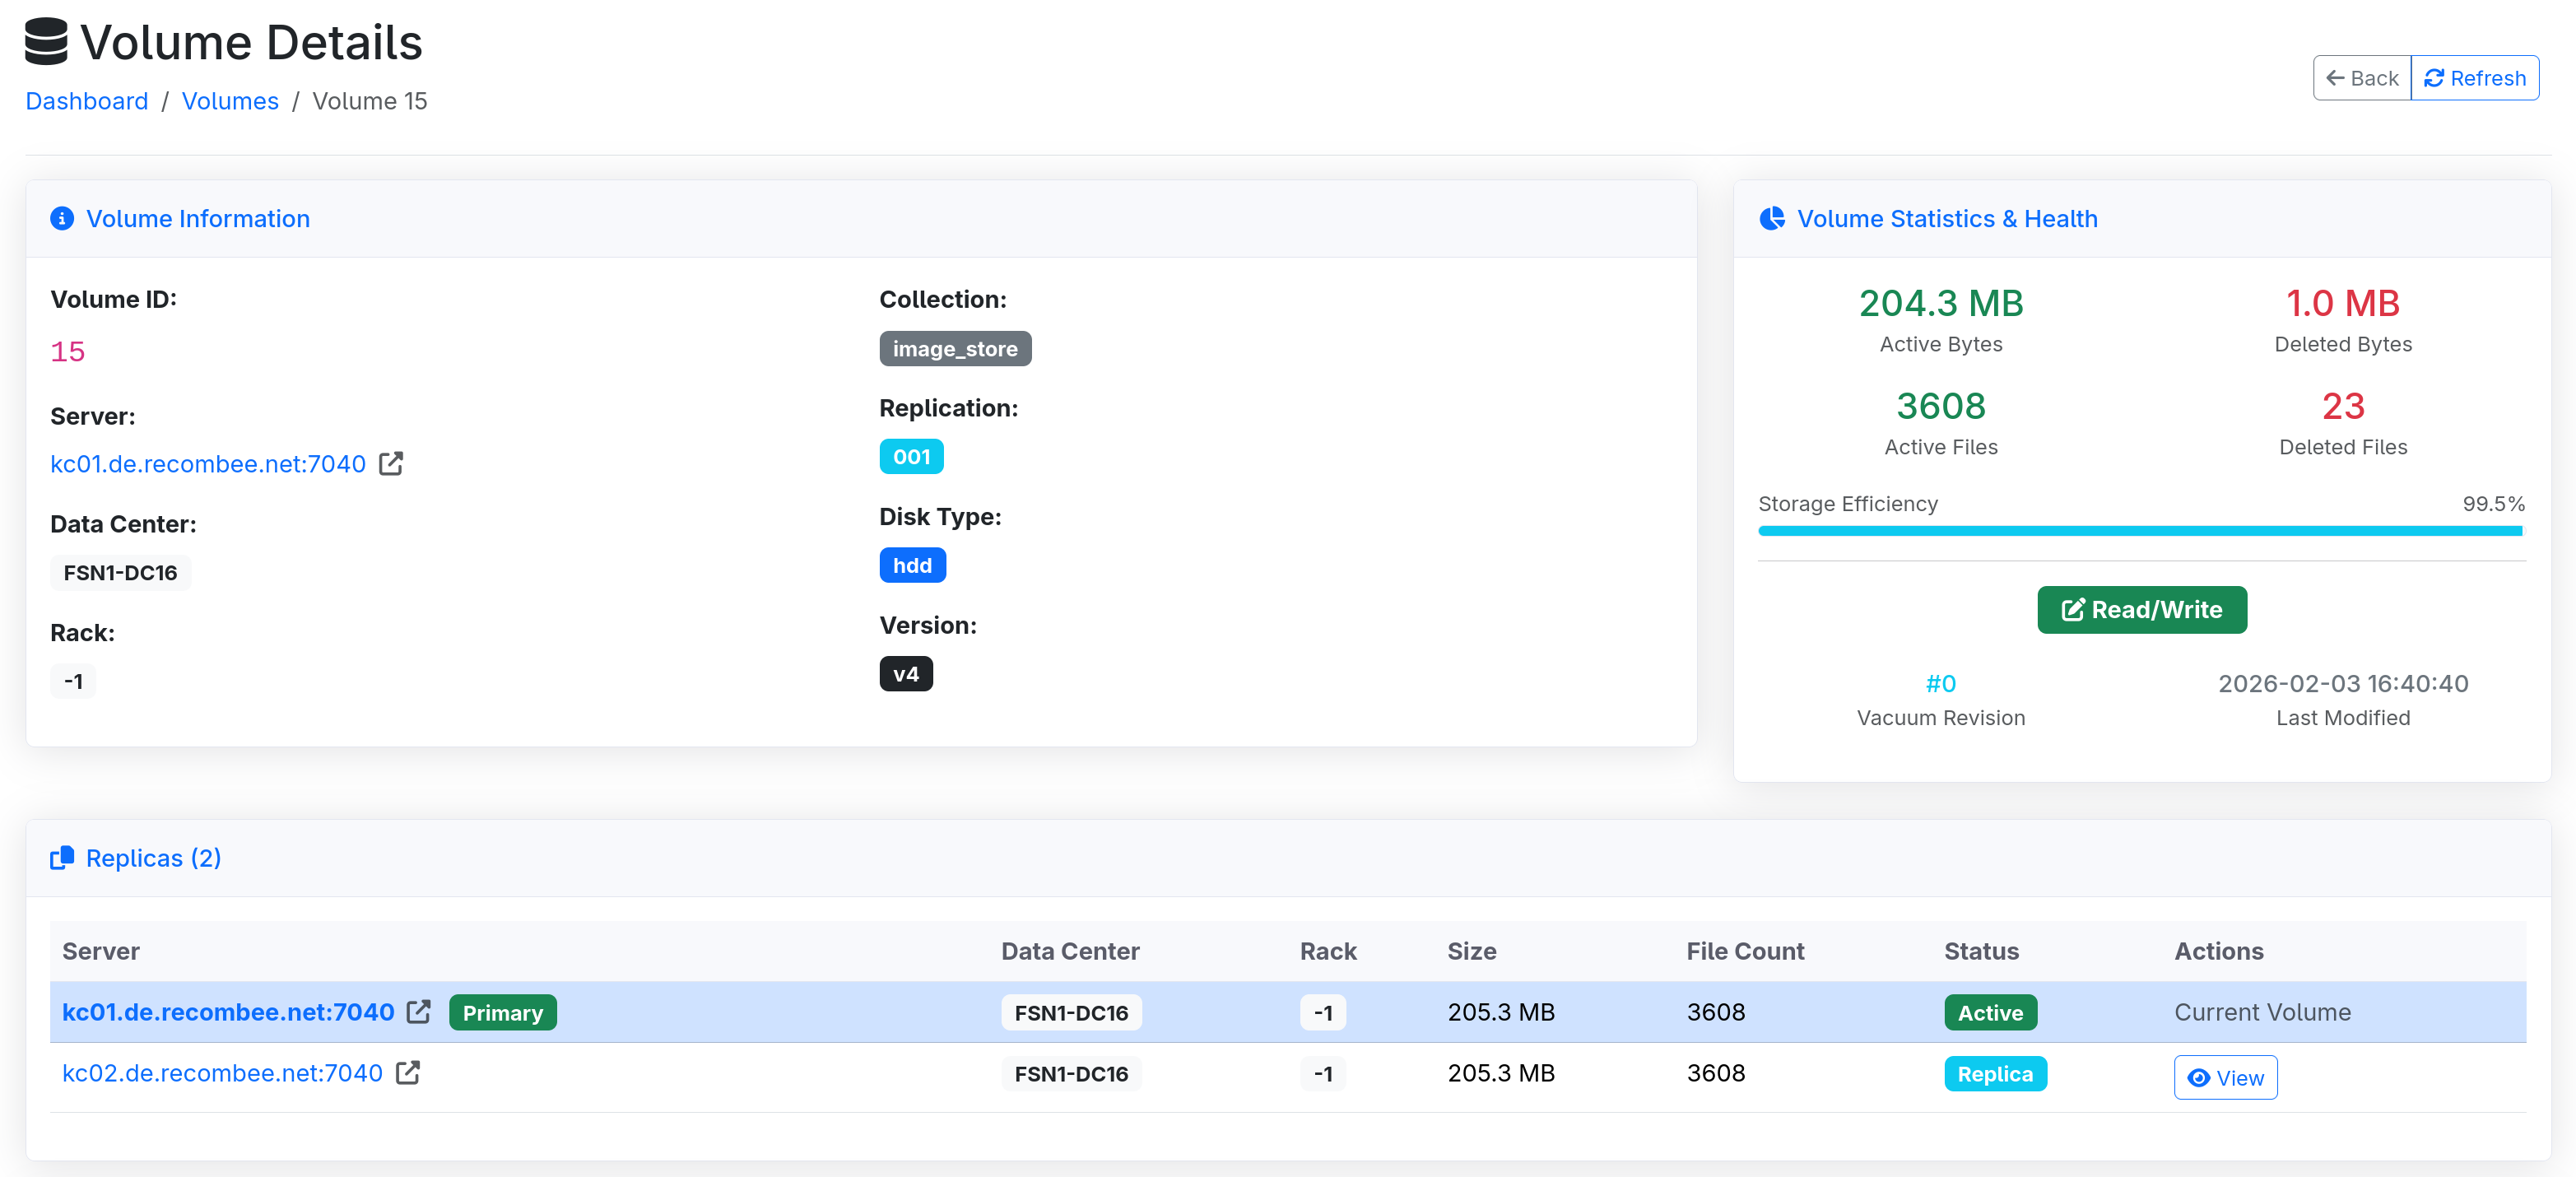
\includegraphics[width=0.85\paperwidth]{images/appendix/wolumeUI.png}
    }
    \caption{Volume UI}
\end{figure}

\begin{figure}[ht]
    \centering
    % This makes a box of 0pt width and puts the image in the center of it
    \makebox[\textwidth][c]{
        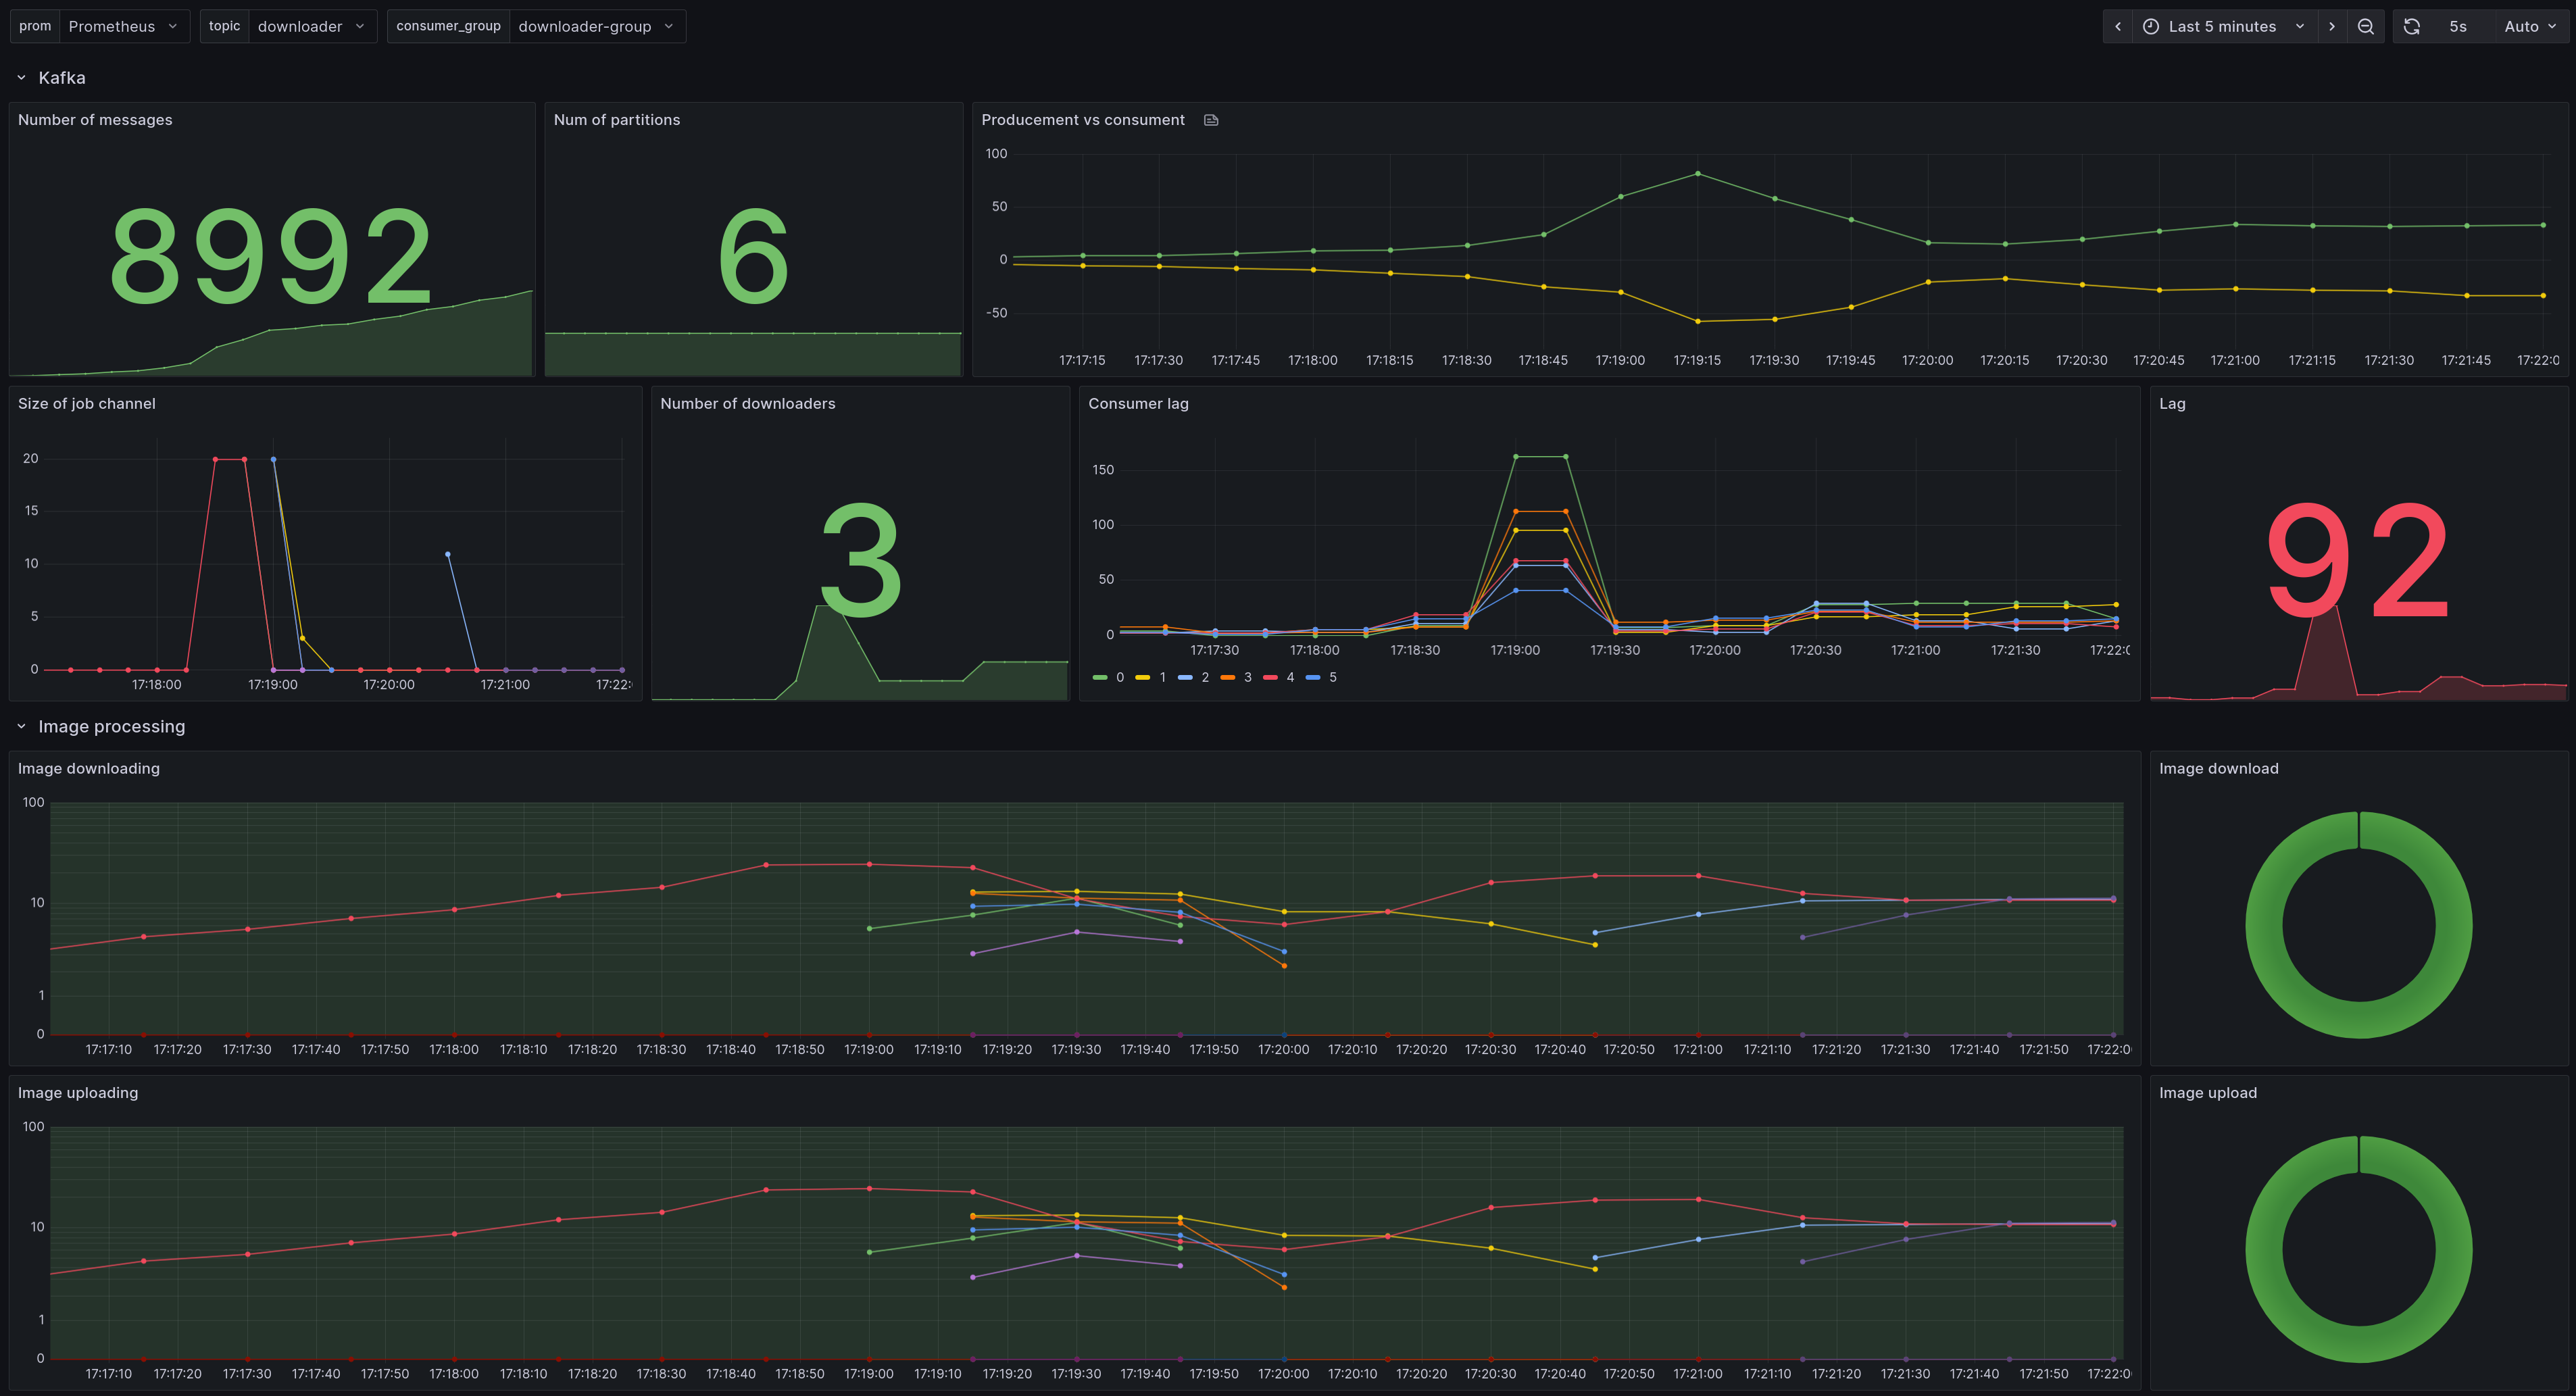
\includegraphics[width=0.85\paperwidth]{images/appendix/grafana.png}
    }
    \caption[Grafana Dowloader dashboard]{Downloader Grafana dashboard. The dashboard displays metrics from Kafka, Image Reactor, and Downloader. From top left: \textit{Number of messages}, \textit{Number of partitions}, \textit{Producer vs consumer}, \textit{Size of job channel}, \textit{Number of downloaders}, \textit{Consumers lag}, \textit{Lag}, \textit{Image downloading}, \textit{Image downloaded}, \textit{Image uploading}, \textit{Image uploaded}.}
\end{figure}

\begin{figure}[ht]
    \centering
    % This makes a box of 0pt width and puts the image in the center of it
    \makebox[\textwidth][c]{
        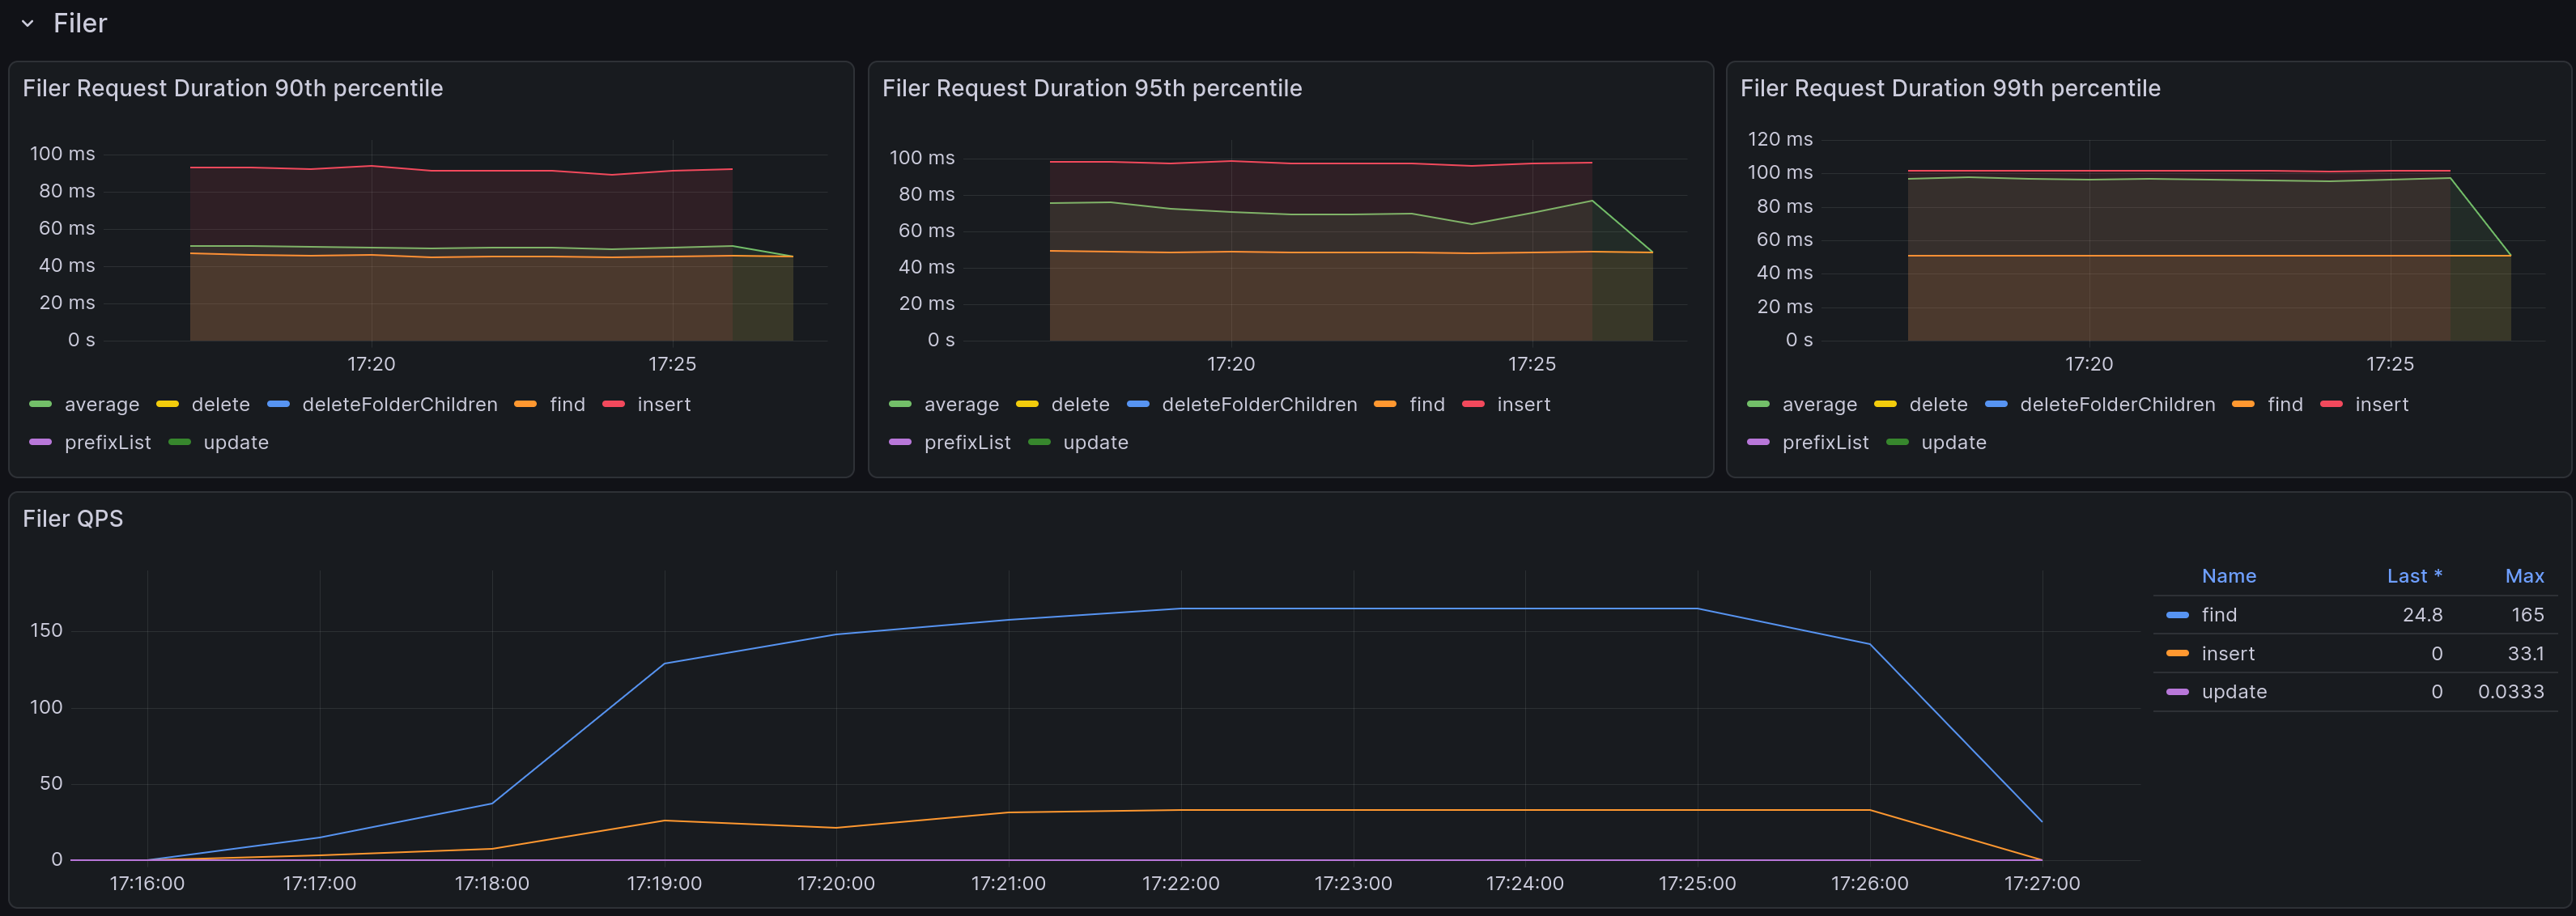
\includegraphics[width=0.85\paperwidth]{images/appendix/seaweedfs_grafana.png}
    }
    \caption[Grafana SeaweedFS dashboard]{SeaweedFS Grafana dashboard. From top left: \textit{Filer Request Duration 90th percentile}, \textit{Filer Request Duration 95th percentile}, \textit{Filer Request Duration 99th percentile}, \textit{Filer QPS}}
\end{figure}

\backmatter % do not remove this command

{
\raggedright
\printbibliography
}

\end{document}
